% @Author: AnthonyKenny98
% @Date:   2019-10-30 22:08:06
% @Last Modified by:   AnthonyKenny98
% @Last Modified time: 2020-04-11 03:28:14

% Define Document Class
\documentclass[
    11pt,           % Font Size
    letterpaper,    % Page Size
    % draft,          % Draft Mode - error checking and no image rendering
    oneside         % Single Sided
]{report}           % Report Mode

% Import custom commands
\RequirePackage{../support/thesis}
\RequirePackage{../support/codestyle}

\loadglsentries{../support/glossary}

%%%%%%%%%%%%%%%%%%%%%%%%%%%%%%%%%%%%%%%%%%%%%%%%%%%%%%%%%%

% DEFINE HEADER & FOOTER: (Name and Page Number)
\pagestyle{fancy}
\setlength{\headheight}{14pt}
\fancyhf{}
\rhead{Anthony J.W. Kenny}
\cfoot{\thepage}

% DEFINE COVER PAGE
\title{\textsc{\Huge{if goingToCrash: don't}\ \\ \Large{RISC-V Architecture for Motion Planning Algorithms in Autonomous UAVs}} \\ 
    \bigskip
    \small{A senior design project submitted in partial fulfillment of the requirements for the degree of Bachelor of Science at Harvard University} \\
\author{Anthony J.W. Kenny \\
        \small{S.B. Candidate in Electrical Engineering} \\ \\
        Faculty Advisor: Vijay Janapa Reddi \\ \\
        Harvard University School of Engineering and Applied Sciences \\
        \small{Cambridge, MA}}
\date{April 10th, 2020 \\ 
    \small{Version: 5.0}}}

\begin{document}

% Cover Page
\maketitle

% PREFACE
\pagenumbering{roman}
\addcontentsline{toc}{chapter}{Preface}

    % ABSTRACT
    \addcontentsline{toc}{section}{Abstract}
    % @Author: AnthonyKenny98
% @Date:   2019-10-30 22:35:34
% @Last Modified by:   AnthonyKenny98
% @Last Modified time: 2019-10-31 10:45:30

\abstract{This thesis aims to design RISC-V computer architecture that supports the fast execution of motion planning algorithms for drone applications. First, the computation of sampling-based motion planning algorithms commonly used in autonomous drones (such as \ac{RRT}, \ac{RRT*}, \ac{PRM}) will be profiled on an unmodified RISC-V processor. From this profiling, common bottlenecks and hotspots in execution will be identified. Based on these results, this project will extend the RISC-V \ac{ISA} and design a modified processor to support the extensions.}
% 78 words ^
    \clearpage

    \addcontentsline{toc}{section}{Dedication}
    % @Author: AnthonyKenny98
% @Date:   2020-04-10 22:14:54
% @Last Modified by:   AnthonyKenny98
% @Last Modified time: 2020-04-10 22:57:08
\renewcommand{\abstractname}{Dedication}
\begin{abstract}
\begin{center}
To my parents, who have always encouraged my academic pursuits, this thesis is dedicated.
\end{center}
\end{abstract}

    % ACKNOWLEDGEMENTS
    \section*{Acknowledgments}
    \addcontentsline{toc}{section}{Acknowledgments}
    % @Author: AnthonyKenny98
% @Date:   2020-04-10 08:17:16
% @Last Modified by:   AnthonyKenny98
% @Last Modified time: 2020-07-22 11:04:49

\renewcommand{\abstractname}{Acknowledgments}
\begin{abstract}
% \begin{center}

To my faculty advisor, Prof. Vijay Janapa Reddi, thank you for your guidance and for inspiring my passion for computer architecture in my Junior year. \\ \\

To Jon Cruz, I couldn't have done this without you. Thank you for introducing me to the tools I needed, for your invaluable advice, and for always being available.  \\ \\

To Patrick Ulrich and the members of my ES100 section, I appreciated our weekly meetings and the fresh perspectives you offered.\\ \\

To Isabella Rhyu, thank you for your help with the more mathematically rigourous parts of this thesis, though I know you found them easy. \\ \\

To Mr. Trombetta, Jeffrey and Balmore. I thank you with heart and soul for providing a home to me for the past three weeks. I regret that our time together was cut short, but I look forward to coming up again soon - I'm sure it will be the same forever.   \\ \\


% \end{center}
\end{abstract}


    % TABLE OF CONTENTS
    \clearpage
    \addcontentsline{toc}{section}{Table of Contents}
    \tableofcontents
    \clearpage

    % ACRONYMNS
    \printglossary[type=\acronymtype,title={List of Acronyms},nopostdot]

    % ALGORITHMS
    \listofalgorithms

    % FIGURES
    \listoffigures

    % TABLES
    \listoftables

    % GLOSSARY OF TERMS
    \newpage
    \printglossary[type=main, title={Glossary of Terms}]

% CHAPTERS

% Chapter 1
\chapter{Introduction}
    \pagenumbering{arabic}                      % Change Page numbering to arabic
    % @Author: AnthonyKenny98
% @Date:   2020-02-20 00:00:23
% @Last Modified by:   AnthonyKenny98
% @Last Modified time: 2020-02-23 14:27:13



\section{Problem Summary}
    % @Author: AnthonyKenny98
% @Date:   2020-02-23 12:45:54
% @Last Modified by:   AnthonyKenny98
% @Last Modified time: 2020-02-23 14:25:32

\subsection{Background}
    \todo[inline]{TODO: Summarize the following points: \\ 
        1) Need for faster execution of motion planning in drones \\
        2) Strategy of specialized hardware \\
        3) RISC-V ISA and its potentials including extendibility \\
    }

    \subsubsection*{Robotics}
        For well over 2000 years, the concept of robotics, albeit not always with such a term, has fascinated humans. As early as the first century A.D., the Greek mathematician and engineer, Heron of Alexandria, described more than 100 different machines and automata in \textit{Pneumatica} and \textit{Automata}\cite{Alexandrinus}. In 1898, Nikola Tesla demonstrated the first radio-controlled vessel. Since then, the world has seen widespread application of robotics in manufacturing, mining, transport, exploration, and weaponry. For the last few decades, robots have operated in controlled, largely unchanging environments (e.g.\ an assembly line) where their environment and movements are largely known \textit{a priori}.
        \newline
        However, in recent years a new generation of autonomous robots has been developed for a wide range of real-world, complex applications. The increasing trend the use of autonomous robots is shown in Figure \ref{fig:useOfAutonomousRobots}. These new robots, unlike those traditional ones described above, are required to adapt to the changing environment in which they operate. As such, they must perform motion planning in real time.

        % @Author: AnthonyKenny98
% @Date:   2020-02-23 12:12:56
% @Last Modified by:   AnthonyKenny98
% @Last Modified time: 2020-02-23 13:56:51

\begin{figure}%[H]
\begin{center}
\missingfigure[figwidth=\linewidth]{Some sort of line/bar graph showing the increasing use of Autonomous robots over time. Need to find}
% 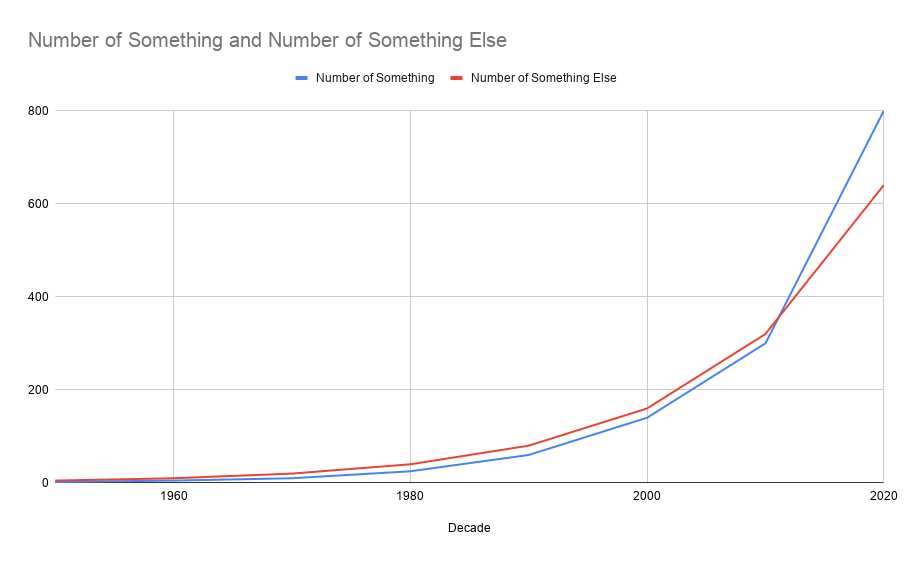
\includegraphics[width=0.8\linewidth]{img/sampleLineGraph.png}
\caption{The use of Autonomous Robots over time}
\label{fig:useOfAutonomousRobots}
\end{center}
\end{figure}

    \subsubsection*{Motion Planning}
        \todo[inline]{TODO: More of an introduction to motion planning.}
        
        Motion Planning refers to the problem of determining how a robot moves through a space to acheive a goal. Chapter \ref{chap:MotionPlanningInSoftware} provides a detailed explanation of motion planning and of \ac{RRT}, a commonly used motion planning algorithm.
        \newline
        On the algorithmic level, motion planning has been extensively studied and many solutions exist. However, current algorithms running on regular \ac{CPU}s are too slow to execute in real time for robots operating in complex environments. Simply solving this problem with more raw computing power, using energy hungry \ac{GPU}s may have merit in tethered robots. On the other hand, untethered applications, such as autonomous drones, where limiting power consumption is a primary concern, this strategy is infeasible.
        
    \subsection*{Hardware Acceleration}
        Specialized hardware designed to perform specific functions can yield significantly higher performance than software running on general purpose processors, and lower power consumption than \ac{GPU}s.
        \todo[inline]{More detail here. Reference prior work}

    \subsubsection{RISC-V}
        \todo[inline]{TODO: Introduction to RISC-V and its merits in this problem}


\subsection{Problem Definition}

    \subsubsection*{Problem Statement}
    \todo[inline]{Revise problem statement}
    Current processors cannot compute motion planning algorithms quickly enough for robots to operate in high complexity environments. Autonomous drones are a specific case of robots requiring real-time motion planning in complex environments. The state-of-the-art strategy of using a Graphics Processing Unit (GPU) to accelerate the execution of these algorithms requires too much power to be cost-effective or feasible for drones to sustain flight for useful periods of time.

    \subsubsection*{End User}
    \todo[inline]{TODO: End User}
    
\section{Prior Work}
    % @Author: AnthonyKenny98
% @Date:   2020-02-23 14:26:30
% @Last Modified by:   AnthonyKenny98
% @Last Modified time: 2020-04-05 08:02:21

\subsection{Hardware Acceleration}
    \Gls{hardware acceleration} refers to the strategy of using computer hardware specifically designed to execute a function more efficiently than can be achieved by software running on a general purpose \gls{CPU}.
    Specialized hardware designed to perform specific functions can yield significantly higher performance than software running on general purpose processors, and lower power consumption than \gls{GPU}s.

    \subsubsection*{Computer Implementation Hierarchy}
        To briefly frame the space in which this thesis operates, consider the typical computer implementation hierarchy, demonstrated in Figure \ref{fig:computerHierarchy}. \textbf{User level applications}, such as Google Chrome, Microsoft Word, and Apple's iTunes, sit at the top of the abstraction hierarchy. These applications are implemented in \textbf{High-Mid Level Languages}, such as C/C++, Python, Java, etc. These programming languages have their own hierarchy, but for the purpose of this thesis, it is sufficient to understand that these programming languages are then compiled into \textbf{Assembly Language}. Assembly language closely follows the execution of instructions on the \textbf{processor}, and is defined by an \textbf{\gls{ISA}}. An \gls{ISA} can be thought of as the contract between software programmers and processor engineers, agreeing what instructions the processor is able to implement. This assembly code is finally loaded into the processor's instruction memory and executed. 
        % @Author: AnthonyKenny98
% @Date:   2020-02-29 23:52:30
% @Last Modified by:   AnthonyKenny98
% @Last Modified time: 2020-04-10 12:37:43
\begin{figure}[H]
\begin{center}
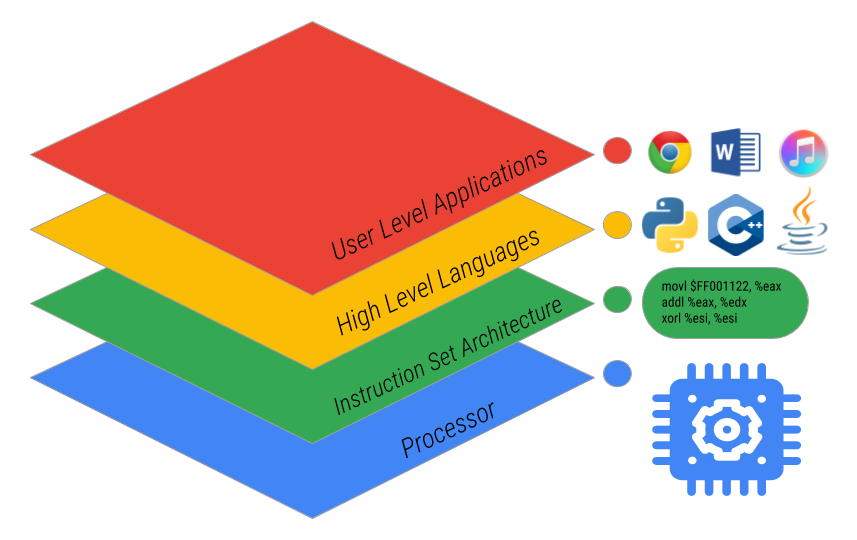
\includegraphics[width=\linewidth]{chapters/chapter1/img/computerHierarchy.png}
\mycaption{Simple Visualization of Computer Implementation Hierarchy}{}
\label{fig:computerHierarchy}
\end{center}
\end{figure}
        As will be outlined in Section \ref{section:projectOverview}, this thesis operates extensively on the lower two levels of this hierarchy, extending an existing \gls{ISA} and building hardware at the processor level that supports these extensions.

    \subsubsection*{Acceleration of Motion Planning}
        Accelerating motion planning with hardware is a fairly well studied problem. \\
        \textit{A Motion Planning Processor on Reconfigurable Hardware} \cite{Atay2006} studied the performance benefits of using \gls{FPGA}-based motion planning hardware as either a motion planning processor, co-processor, or collision detection chip. It targeted the feasibility checks of motion planning (largely collision detection) and found their solution could build a roadmap using the \gls{PRM} algorithm up to 25 times faster than a Pentium-4 3Ghz CPU could. \\
        In \textit{A Programmable Architecture for Robot Motion Planning Acceleration} \cite{Murray}, Murray et al. built on the work of the aformentioned paper, to accelerate several aspects of motion planning in an efficent manner. \\
        \textit{FPGA based Combinatorial Architecture for Parallelizing RRT} \cite{Malik2015} studies the possibility of building architecture to allow multiple \gls{RRT}s to work simultaneously to uniformly explore a map. Taking advantage of hardware parallelism allows systems such as this to compute more information per clock cycle. \\
        Finally, in the paper \textit{Robot Motion Planning on a Chip} \cite{Murrayb}, Murray et al. describe a method for contructing robot-specific hardware for motion planning, based on the method of constructing collision detection circuits for \gls{PRM} that are completely parallelised, such that edge collision computation performance is independent of the number of edges in the graph. With this method, they could compute motion plans for a 6-degree-of-freedom robot more than 3 orders of magnitude faster than previous methods.

    \subsection{RISC-V}
    \subsubsection{Extending RISC-V}
    RISC-V is designed cleverly in a modular way, with a set of base instruction sets and a set of standard extensions. As a result, processors can be designed to only implement the instruction groups it requires, saving time, space and power on instructions that won't be used. In addition, another goal of RISC-V is to provide a basis for more specialized instruction-set extensions or more customized accelerators. This is described in the most recent \textit{RISC-V Instruction Set Manual} \cite{Waterman2019}. This is a powerful feature, as it does not break any software compatability, but allows for designers to easily follow the steps outlined in Figure \ref{fig:extendingRISCV}. From a \gls{hardware acceleration} point of view, this is particularly useful as it allows the designer to directly invoke whatever functional unit or accelerator they implement from assembly code.
    % @Author: AnthonyKenny98
% @Date:   2020-03-01 10:28:34
% @Last Modified by:   AnthonyKenny98
% @Last Modified time: 2020-03-01 10:32:45
\begin{figure}[H]
\begin{center}
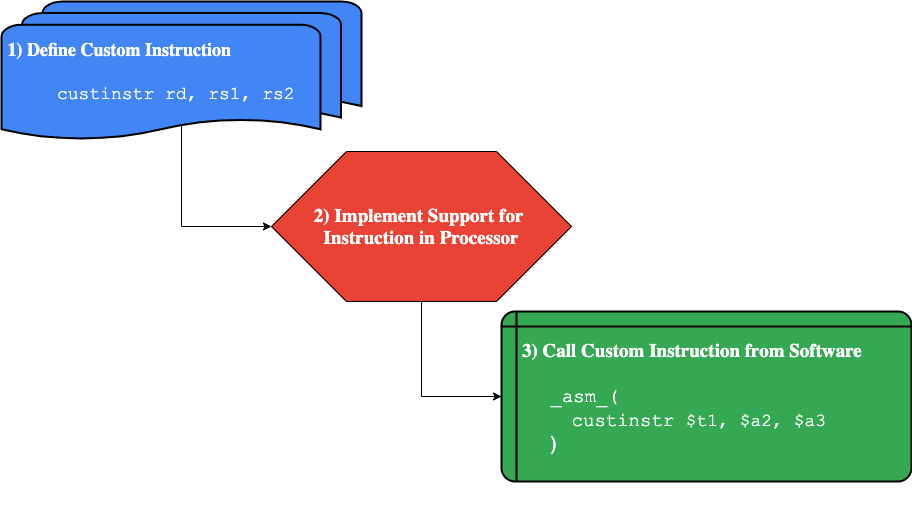
\includegraphics[width=0.9\linewidth]{chapters/chapter1/img/extendingRISCV.png}
\caption{Typical Process of Adding Non-Standard Extension to RISC-V ISA}
\label{fig:extendingRISCV}
\end{center}
\end{figure}

    \subsubsection{Accelerating RISC-V Processors}
    Having only been released in 2011, RISC-V is still a relatively unexplored opportunity for non-education applications. However, it shows promise in the commercial space, with Alibaba recently developing the Xuantie, a 16-core, 2.5GHz processor, currently the fastest RISC-V processor. Recently there has been promising research into accelerating computationally complex applications, particularly in edge-computing, with RISC-V architecture. \\
    \textit{Towards Deep Learning using TensorFlow Lite on RISC-V}, a paper co-written by the faculty advisor of this thesis, V.J. Reddi, presented the software infrastructure for optimizing the execution of neural network calculations by extending the RISC-V ISA and adding processor support for such extensions. A small number of instruction extensions achieved coverage over a wide variety of speech and vision application deep neural networks. Reddi et al. were able to achieve an 8 times speedup over a baseline implementation when using the extended instruction set.
    \textit{GAP-8: A RISC-V SoC for AI at the Edge of the IoT} proposed a programmable RISC-V computing engine with 8-core and convolutional neural network accelerator for power efficient, battery operated, IoT edge-device computing with order-of-magnitude performance improvements with greater energy efficiency. \\



\section{Project Overview}
    % @Author: AnthonyKenny98
% @Date:   2020-02-23 14:27:21
% @Last Modified by:   AnthonyKenny98
% @Last Modified time: 2020-02-23 14:28:10

\subsection{Proposed Solution}
    \todo[inline]{Proposed Solution}


\subsection{Project Specifications}
    \todo[inline]{Project Specifications}

\subsection{Project Structure}
    \todo[inline]{Project Structure/Timeline}



\newpage

    \lhead{Chapter \thechapter}                 % Include Chapter name on subsequent headers


% Chapter 2
\chapter{Motion Planning in Software}
    \label{chap:MotionPlanningInSoftware}
    % @Author: AnthonyKenny98
% @Date:   2020-02-22 15:42:12
% @Last Modified by:   AnthonyKenny98
% @Last Modified time: 2020-04-05 17:17:11

The first objective of this thesis is to identify a typical motion planning algorithm, profile its execution, and determine computational bottlenecks.\todo{Update once I have properly defined goals and objectives}

This chapter introduces the concept of motion planning and details the process of implementing and analysing \glsfirst{RRT}, a commonly used algorithm, to identify its computational bottlenecks.\\

\section{Motion Planning Background} 
\label{section:motion_planning_background}
    % @Author: AnthonyKenny98
% @Date:   2020-04-04 10:01:40
% @Last Modified by:   AnthonyKenny98
% @Last Modified time: 2020-04-05 10:56:20

A funny paradox in computer science is the fact that it is relatively easy to teach a computer to perform tasks that humans find very complicated, but extremely difficult to program one to execute functions that humans master during infancy. Consider, it was as early as 1949 that Claude Shannon presented his paper \textit{Programming a Computer for Playing Chess}\cite{Shannon1950}, and by 1997 the \textit{Deep Blue} computer defeated Garry Kasparov, reigning world champion, in a six game chess match.\cite{Campbell2002} Compare that with some of the most advanced autonomous humanoid robots to date displaying dexterity only comparable with that of a toddler. The task of finding a collision free path, performed constantly without thought by a human, is an example of this paradigm. For a robot to compute a collision free path, it relies on a set of Motion Planning Algorithms.

Motion Planning Algorithms refer to the set of algorithms that find possible sequences of valid \gls{configuration}s for a robot in a space. In plain English, they are algorithms that determine the movements a robot can make in a map, with the intent of eventually finding a path from one point to another. 

\subsection{Key Concepts}
    \subsubsection{\Gls{workspace}}
    The \gls{workspace}, more loosely known as the \textbf{map}, is the space which the robot and obstacles occupy. Obviously, \textbf{obstacles} refer to anything with which the robot cannot intersect.
    
    \subsubsection{Configuration}
    A configuration describes the position, orientation, and pose of the robot. The complexity of a robot's configuration is therefore dependant on the dimension of the \gls{workspace}, the complexity of the robot itself, and in what level of detail the robot must be represented. For example:
    \begin{itemize}
        \item Most simply, a robot can be represented as a point by the Cartesian coordinates $(x,y)$ \gls{2D} space and $(x,y,z)$ in \gls{3D} space.
        \item More realistically, a robot such as a drone may be represented in \gls{3D} by an origin point $(x,y,z)$ and 3 Euler angles $(\alpha,\beta,\gamma)$ describing its orientation.
        \item In a more complex form, a fixed base robot with $N$ \glsfirst{DOF} would require an $N$-dimensional configuration.
    \end{itemize}

    % @Author: AnthonyKenny98
% @Date:   2020-04-04 11:13:58
% @Last Modified by:   AnthonyKenny98
% @Last Modified time: 2020-04-04 12:09:59
% @Author: AnthonyKenny98
% @Date:   2020-02-29 17:30:44
% @Last Modified by:   AnthonyKenny98
% @Last Modified time: 2020-04-03 14:28:30
\begin{figure}[H]
\begin{center}
\begin{tabular}{cc}

    % Subfigure A
    \begin{subfigure}{0.4\textwidth}
    \begin{center}
    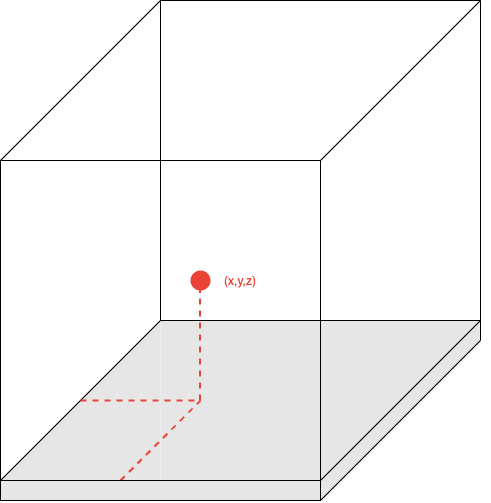
\includegraphics[width=\linewidth]{chapters/chapter2/img/motionPlanning/3DPointConfiguration.png}
    \caption{A robot represented by just a point in 3D space, requiring only 3 Cartesian coordinate $(x,y,z)$ points to describe its \gls{configuration}}
    \label{subfig:3DPointConfig}
    \end{center}
    \end{subfigure}
    &
    % 
    % Subfigure B
    \begin{subfigure}{0.4\textwidth}
    \begin{center}
    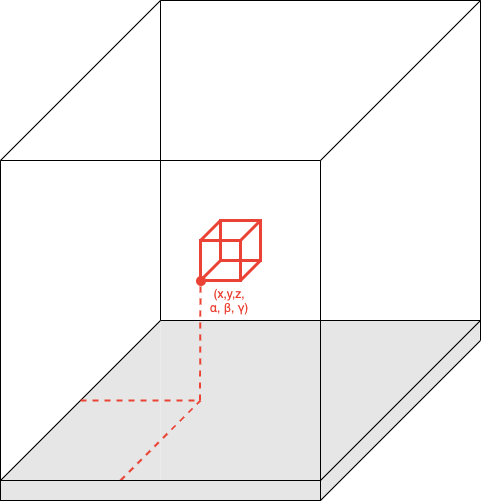
\includegraphics[width=\linewidth]{chapters/chapter2/img/motionPlanning/3DCubeConfiguration.png}
    \caption{A robot represented as a cube in 3D space, now requiring 3 Euler angles $(\alpha, \beta, \gamma)$ along with the original Cartesian coordinates.}
    \label{subfig:3DCubeConfig}
    \end{center}
    \end{subfigure} \\
\end{tabular}
    % Caption and Label
    \caption{Example of 2 Robot Configurations in 3D Space for Motion Planning Purposes}
    \label{fig:configuration}

\end{center}
\end{figure}

    \subsubsection{Occupancy Grid Map}
    An \glsfirst{OGM} is a method of representing the obstacles present in a \gls{workspace}. Obstacles are often irregularly shaped and computing collisions with such obstacles is near impossible. Therefore, the \gls{workspace} is discretized into grids and grids containing any part of the obstacle are markes as occupied, even if only a small part of the grid is occupied. An \gls{OGM} will more accurately represent a \gls{workspace} with a higher resolution, shown in Figure \ref{fig:OGM}.

    % @Author: AnthonyKenny98
% @Date:   2020-04-04 12:27:50
% @Last Modified by:   AnthonyKenny98
% @Last Modified time: 2020-04-06 15:13:14
% @Author: AnthonyKenny98
% @Date:   2020-04-04 11:13:58
% @Last Modified by:   AnthonyKenny98
% @Last Modified time: 2020-04-04 12:09:59
% @Author: AnthonyKenny98
% @Date:   2020-02-29 17:30:44
% @Last Modified by:   AnthonyKenny98
% @Last Modified time: 2020-04-03 14:28:30
\begin{figure}[H]
\begin{center}
\begin{tabular}{cc}

    % Subfigure A
    \begin{subfigure}{0.4\textwidth}
    \begin{center}
    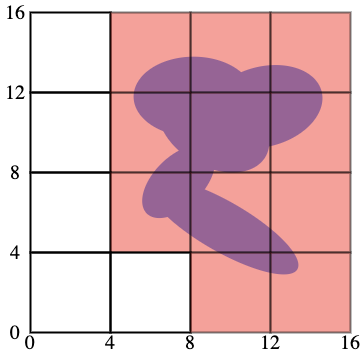
\includegraphics[width=\linewidth]{chapters/chapter2/img/motionPlanning/OGMlowres.png}
    \caption{}
    \label{subfig:OGM_A}
    \end{center}
    \end{subfigure}
    &
    % 
    % Subfigure B
    \begin{subfigure}{0.4\textwidth}
    \begin{center}
    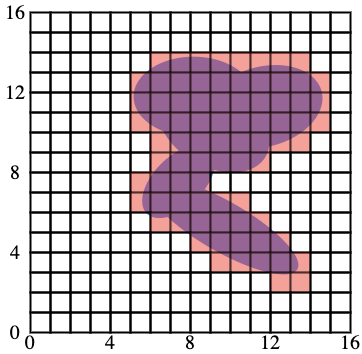
\includegraphics[width=\linewidth]{chapters/chapter2/img/motionPlanning/OGMhighres.png}
    \caption{}
    \label{subfig:OGM_B}
    \end{center}
    \end{subfigure} \\
\end{tabular}
    % Caption and Label
    \mycaption{Occupancy Grid Maps for a (16$\times$16) Workspace of Different Resolutions}{. Figure \ref{subfig:OGM_A} shows how an OGM with low resolution, while simpler to construct and analyse, will over-represent the obstacle density of a workspace. Figure \ref{subfig:OGM_B} shows how a higher resolution will more accurately reflect the obstacles of a workspace.}
    \label{fig:OGM}

\end{center}
\end{figure}

\subsection{Algorithms}
    
    \subsubsection{Scope}
    \todo[inline,caption=Finish Scope]{Part of the problem, it is not about sensing obstacles, building map, or finding shortest path. It is merely about exploring the space and building a tree of possible paths}

\todo[inline]{Finish this Section, should describe why I chose RRT}


\newpage
\section{Implementation of RRT}
\label{section:rrt}
    % @Author: AnthonyKenny98
% @Date:   2020-02-22 15:53:59
% @Last Modified by:   AnthonyKenny98
% @Last Modified time: 2020-04-05 13:31:53

% INTRO
\glsfirst{RRT} is an algorithm designed to efficiently build a tree of collision-free paths in a high-complexity environment. The algorithm randomly samples points, draws an edge from the nearest currently existing node in the tree, to grow the tree in the space. It is inherently biased to grow towards large unsearched areas of the workspace. RRT was developed by S. LaVelle\cite{LaValle1998} and J. Kuffner\cite{LaValle2001}. It is used in autonomous robotic motion planning problems such as autonomous drones.

% ALGORITHM
\subsection{Algorithm}

    % SCOPE OF ALGORITHM
    \subsubsection{Scope}
        \gls{RRT} takes an \glsfirst{OGM} as its input. This \gls{OGM} may be built and updated using \gls{a priori} knowledge, sensor data from the robot, and other inputs. \gls{RRT} will output a tree of collision free paths toward the goal, as demonstrated in Figure \ref{fig:rrt_scope}. \textbf{It does not calculate the fastest path from that tree}; that can be accomplished using algorithms such as \Gls{dijkstra's algorithm}.

        % @Author: AnthonyKenny98
% @Date:   2020-04-05 10:54:20
% @Last Modified by:   AnthonyKenny98
% @Last Modified time: 2020-04-05 11:05:47

\begin{figure}[H]
\begin{centering}
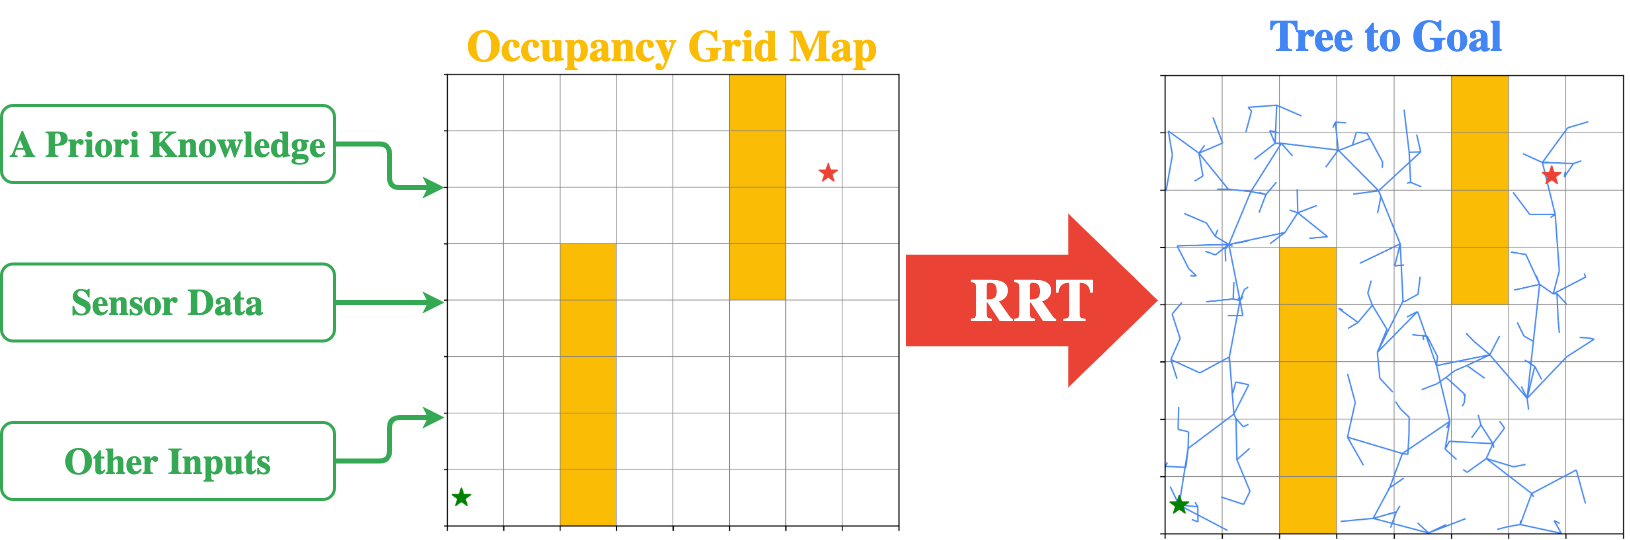
\includegraphics[width=\linewidth]{chapters/chapter2/img/RRT-Scope.png}
\caption[Scope of the RRT Algorithm]{Scope of the RRT Algorithm: Takes an \gls{OGM} as input and outputs a tree of collision free paths through that \gls{OGM}. The tree is shown in blue on the right.} 
\label{fig:rrt_scope}
\end{centering}
\end{figure}

    % BASIC RRT - BUILDING THE TREE
    \subsubsection{Building the Tree}

        Put simply, \gls{RRT} finds a path from start to finish by randomly exploring a workspace.
        Put more technically, it builds a tree of possible \glspl{configuration} (also known as a graph), connected by edges, for a robot of some physical description. It does so by selecting random \glspl{configuration} and adding them to the graph. 
        From this graph, a path from the initial \gls{configuration} to some goal \gls{configuration} can be found, given a high enough number of iterations. As such, \gls{RRT} can be considered \gls{probabilistically complete}.
        The pseudo-code for \gls{RRT} can be seen in Algorithm \ref{algorithm:rrt}
        
        % RRT Algorithm
        % @Author: AnthonyKenny98
% @Date:   2020-02-27 10:55:29
% @Last Modified by:   AnthonyKenny98
% @Last Modified time: 2020-02-27 15:45:23

\begin{algorithm}[H]
    \caption{Rapidly-Exploring Random Tree in Free Configuration Space}
    \SetAlgoLined
    \SetArgSty{textnormal}
    \begin{tabular}{l l}
    \textbf{Inputs:}    & Initial configuration $q_{init}$,\\ 
                        & Number of nodes in graph $K$, \\
                        & Incremental Distance $\Delta q$ \\
    \textbf{Output:}    & RRT Graph $G$ with $K$ configurations \& edges \\
    \end{tabular}

        $G$.init()\;
        \For{$k = 1$ to $K$}{
            $q_{rand} \leftarrow $ randomConfiguration(); \\
            $q_{near} \leftarrow $ nearestVertex($q_{rand}$, $G$); \\
            $q_{new} \leftarrow $ newVertex($q_{near}$, $q_{rand}$, $\Delta q$); \\
            $G$.addVertex($q_{new}$); \\  
            $G$.addEdge($q_{near}$, $q_{new}$);
        }
\label{algorithm:rrt}
\end{algorithm}

        % Explanation of Algorithm, referencing visual step by step figure
        Algorithm \ref{algorithm:rrt} can be visually represented in Figure \ref{fig:rrt-step-by-step}. Consider a \gls{2D} robot operating in a \gls{2D} workspace. A Graph $G$ is initialized containing an initial \gls{configuration}, $q_{init}$, with constraints on the number of nodes that the graph can hold, $K$, and the maximum distance between two nodes, $\Delta q$. This is shown in Sub-figure \ref{subfig:rrt-step-by-step-A}. A random \gls{configuration} for the robot, $q_{rand}$ is generated (\ref{subfig:rrt-step-by-step-B}). The nearest existing \gls{configuration} in $G$, $q_{near}$, is found. (In the first iteration, $q_{near} = q_{init}$, shown in Sub-figure \ref{subfig:rrt-step-by-step-C}). The distance between $q_{near}$ and $q_{rand}$ is calculated. If this distance is less than $\Delta q$, $q_{new} = q_{rand}$. If not, $q_{new}$ is selected, typically by moving by $\Delta q$ from $q_{near}$ towards $q_{rand}$ (\ref{subfig:rrt-step-by-step-C}). $q_{new}$ is then added to $G$. This is repeated for $K$ \gls{configuration}s.
        \todo[inline]{This is all really ugly and should be explained better}

        % Step By Step RRT Figure
        % @Author: AnthonyKenny98
% @Date:   2020-02-27 14:22:10
% @Last Modified by:   AnthonyKenny98
% @Last Modified time: 2020-02-27 15:36:30

\begin{figure}[H]
\begin{center}
\begin{tabular}{c c}

    % Subfigure A
    \begin{subfigure}{0.45\textwidth}
    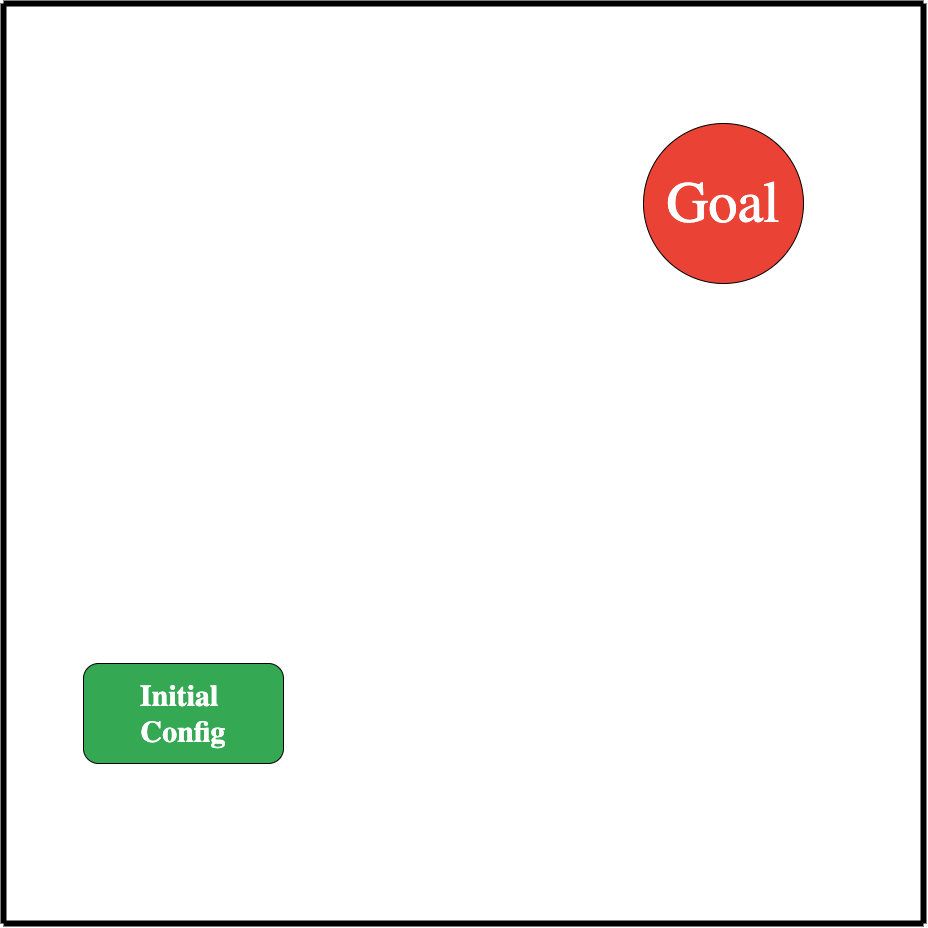
\includegraphics[draft=false,width=\linewidth]{chapters/chapter2/img/RRT_step_by_step-A.png}
    \caption{Graph $G$ contains only $q_{init}$ \newline}
    \label{subfig:rrt-step-by-step-A}
    \end{subfigure} &
    % 
    % Subfigure B
    \begin{subfigure}{0.45\textwidth}
    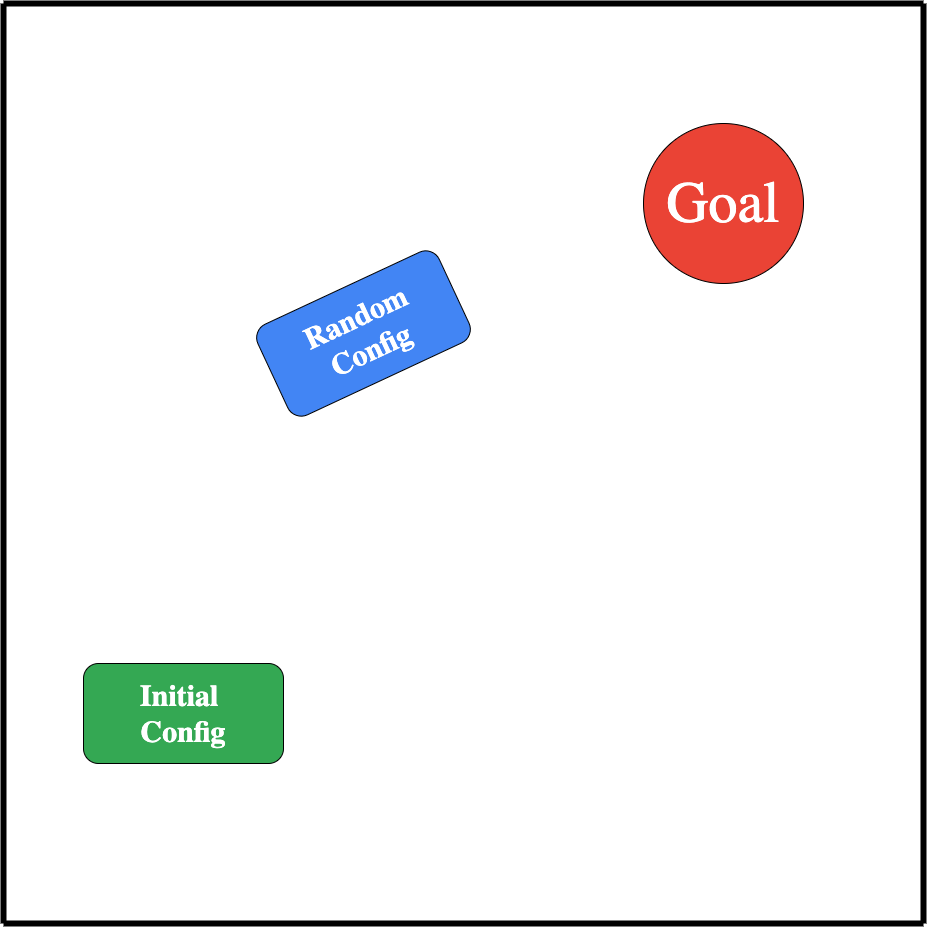
\includegraphics[draft=false,width=\linewidth]{chapters/chapter2/img/RRT_step_by_step-B.png}
    \caption{The first random configuration, $q_{rand}$, is generated}
    \label{subfig:rrt-step-by-step-B}
    \end{subfigure} \\ \\

    % Subfigure C
    \begin{subfigure}{0.45\textwidth}
    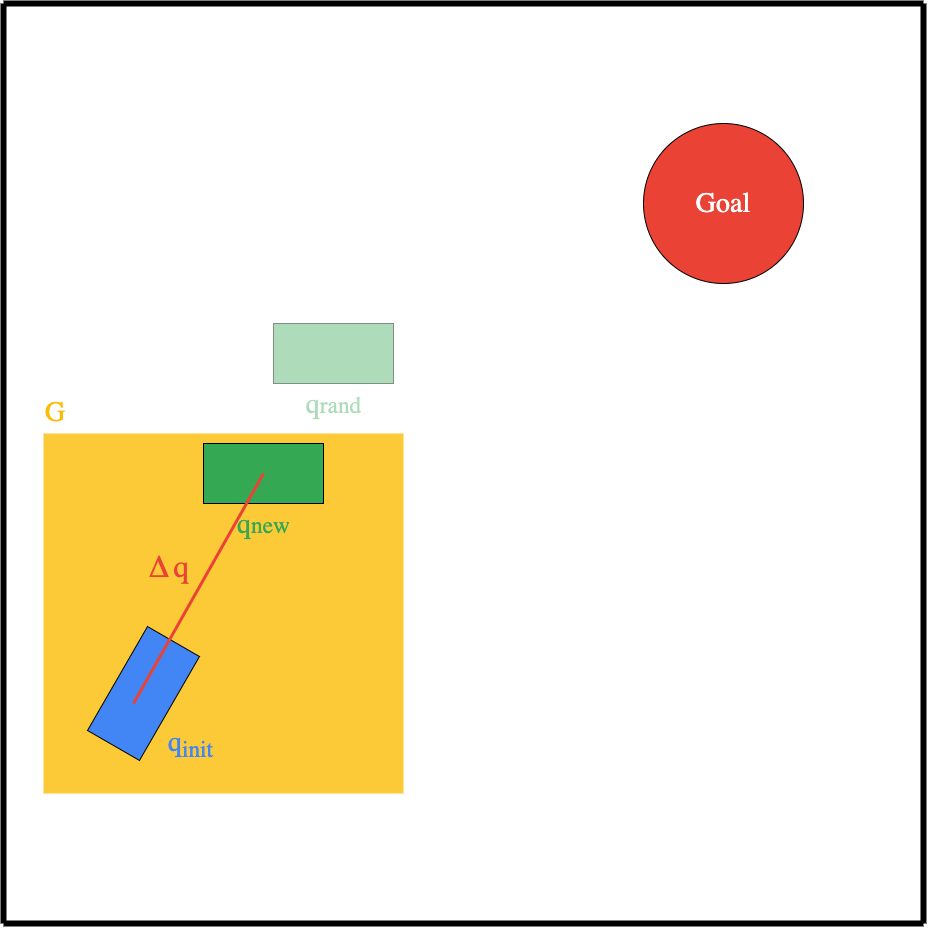
\includegraphics[draft=false,width=\linewidth]{chapters/chapter2/img/RRT_step_by_step-C.png}
    \caption{In first iteration, $q_{near} = q_{init}$. Distance between $q_{init}$ and $q_{rand}$ is greater than $\Delta q$, so $q_{new}$ is generated and added to $G$}
    \label{subfig:rrt-step-by-step-C}
    \end{subfigure} &
    % 
    % Subfigure D
    \begin{subfigure}{0.45\textwidth}
    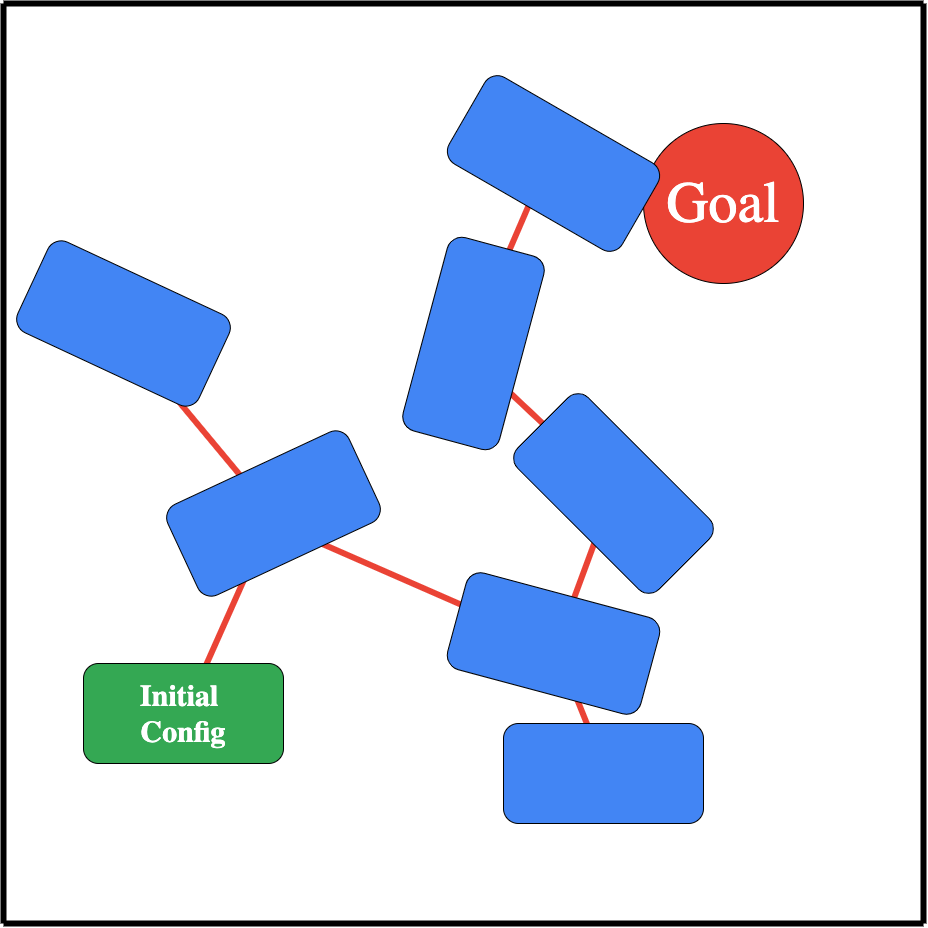
\includegraphics[draft=false,width=\linewidth]{chapters/chapter2/img/RRT_step_by_step-D.png}
    \caption{This is repeated $K$ times. For $G$, $K=10$, and the red line represents the edges between configurations}
    \label{subfig:rrt-step-by-step-D}
    \end{subfigure}

\end{tabular}
    
    % Caption and Label
    \caption{Step by step demonstration of \ac{RRT} Algorithm for 2D robot in 2D space}
    \label{fig:rrt-step-by-step}
\end{center}
\end{figure}
        \todo{Redo this diagram}

    % COLLISION DETECTION
    \subsubsection{Collision Detection}

        Algorithm \ref{algorithm:rrt} shows how \gls{RRT} builds a graph of possible \gls{configuration}s connected by edges in a completely free \gls{configuration} space. However, in real-world applications, a robot's \gls{workspace} space often contains obstacles. As such, collision detection must be included in the algorithm. The two types of collisions the algorithm must check for are \textit{configuration collisions} (those where the robot would collide with an obstacle in a given \gls{configuration}) and \textit{edge collisions} (where the robot would collide when moving between two collision free \gls{configuration}s).

        The RRT with \gls{configuration} and edge collision detection can be seen in Algorithm \ref{algorithm:rrt_collision}. The method of implementing \gls{RRT} with collision detection to model a drone in 3D space is detailed in Section \ref{section:implementation}.

        % @Author: AnthonyKenny98
% @Date:   2020-02-27 18:27:36
% @Last Modified by:   AnthonyKenny98
% @Last Modified time: 2020-04-03 14:28:31
\bigskip
\begin{algorithm}[H]
    \caption{Rapidly-Exploring Random Tree with Collision Detection}
    \SetAlgoLined
    \SetArgSty{textnormal}
    \begin{tabular}{l l}
    \textbf{Inputs:}    & Initial \gls{configuration} $q_{init}$,\\ 
                        & Number of nodes in graph $K$, \\
                        & Incremental Distance $\Delta q$, \\
                        & Space $S$ containing obstacles \\
    \textbf{Output:}    & RRT Graph $G$ with $K$ \gls{configuration}s $[q]$ \& edges $[e]$ \\
    \end{tabular}

        $G$.init()\;
        \For{$k = 1$ to $K$}{
            \While { !\text{pointCollision}($q_{new}$) } {
                $q_{rand} \leftarrow $ randomConfiguration(); \\
                $q_{near} \leftarrow $ nearestVertex($q_{rand}$, $G$); \\
                $q_{new} \leftarrow $ newVertex($q_{near}$, $q_{rand}$, $\Delta q$); \\
            }
            $e_{new} \leftarrow $ newEdge($q_{near}, q_{new}$) \\
            \eIf{\text{!edgeCollision($e_{new}$)}} {
                $G$.addVertex($q_{new}$); \\  
                $G$.addEdge($q_{near}$, $q_{new}$);
            }{
                $k = k-1$;
            }
        }
\label{algorithm:rrt_collision}
\end{algorithm}
\bigskip

\newpage

% IMPLEMENTATION OF RRT
\subsection{Implementation}\label{section:implementation}
    
    % TECHNICAL SPECIFICATIONS
    \subsubsection{Technical Specifications}

        With \gls{RRT} selected as the benchmark algorithm against which to test specialised hardware, this project required an implementation of the algorithm that satisfied the following criteria.\todo{Better RRT Implementation introductory sentence}

        % Tech Spec Table
        \begin{table}[H]
\begin{center}
\begin{tabular}{|p{.3\linewidth}|p{.64\linewidth}|}
    \hline
    Requirement             & Description and Justification \\
    \hline
    C/C++ Implementation    & As outlined in Section \ref{subsection:project_structure}, the critical step in determining the design of specialized hardware to accelerate \ac{RRT} is CPU performance analysis of the algorithm to determine computational hot-spots. Implementations in C allow for the use of certain CPU profiling tools, described in Section \ref{subsubsection:vtune}, unlike higher-level languages such as Python. \\
    \hline
    Models Drone as Point   & In reality, implementing \ac{RRT} for a drone would model the robot as a \ac{3D} object defined by coordinates $\{x, y, z\}$ and Euler angles $\{\alpha, \beta, \gamma \}$. However, for simplicity's sake, modelling the drone as a point defined by coordinates $\{x, y, z\}$ will suffice. Time permitting, this could be revisited. \todo[inline]{Change this based on whether time does permit} \\
    \hline
    Mirrors Algorithm       & In order for the results of CPU performance analysis to be easy to understand, software implementation of \ac{RRT} should call functions that mirror the functions described in Algorithms \ref{algorithm:rrt} and \ref{algorithm:rrt_collision}. \\
    \hline
\end{tabular}
\caption{Technical Specifications for \ac{RRT} Implementation}
\label{table:RRT_Tech_Specs}
\end{center}
\end{table}
\todo[inline]{Improve this table}

        The original intention was to find an existing implementation of RRT that could fulfill these requirements. Most open source implementations found online were in Python, and all those implemented in C were unsuitable, as they had extraneous \gls{GUI}s, reliance on external \gls{API}s, and other features that would distort analysis of algorithmic hot-spots. Appendix \ref{section:rrt_appendix_existing_implementations} is shows an evaluation of existing implementations.\cite{RoboJackets2019}\cite{Planning2019}\cite{Sourishg2017}\cite{Vss2sn2019}.

        As a result, it was necessary to build a C implementation of RRT from the ground up that satisfied the requirements in Table \ref{table:RRT_Tech_Specs}. It can be found in this project's GitHub repository. It follows Algorithm \ref{algorithm:rrt_collision} closely. For monitoring correctness, I build in an optional \gls{GUI} that shows the tree, starting node, and obstacles.

    \subsubsection*{Modelling a \gls{UAV} for RRT}

    \subsubsection{Implementation in 2D}
    The first step was to implement RRT with a 2-Dimensional workspace. \todo[inline]{More detail}
    % @Author: AnthonyKenny98
% @Date:   2020-02-23 14:14:12
% @Last Modified by:   AnthonyKenny98
% @Last Modified time: 2020-03-01 08:06:12


\begin{figure}[H]
\begin{center}
\begin{tabular}{c  c}
    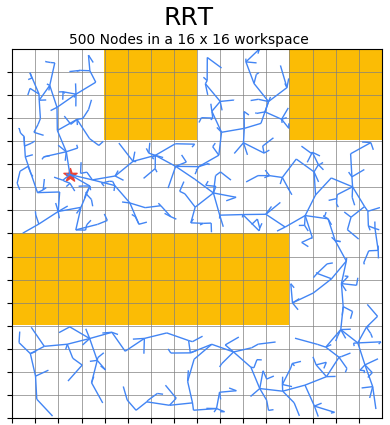
\includegraphics[width=0.45\linewidth]{chapters/chapter2/img/rrt_2d_1.png} & 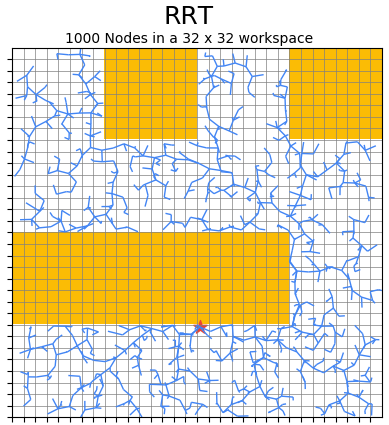
\includegraphics[width=0.45\linewidth]{chapters/chapter2/img/rrt_2d_2.png} \\
    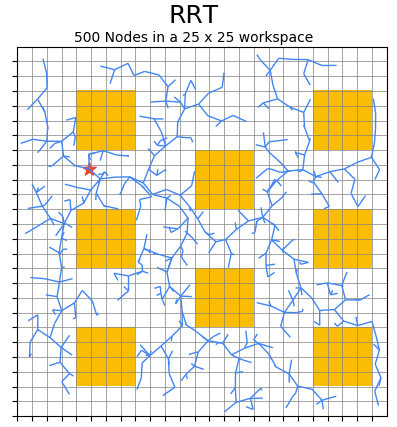
\includegraphics[width=0.45\linewidth]{chapters/chapter2/img/rrt_2d_3.png} & 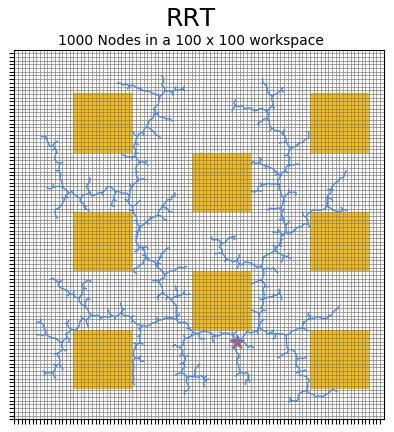
\includegraphics[width=0.45\linewidth]{chapters/chapter2/img/rrt_2d_4.png}
    \end{tabular}
    \caption{2D RRT Implementation shown by \ac{GUI}}
    \label{figure:2DrrtGui}
\end{center}
\end{figure}

    \subsubsection{Implementation in 3D}
    \todo[inline]{Describe implementation in 3D}
    % @Author: AnthonyKenny98
% @Date:   2020-02-23 14:14:12
% @Last Modified by:   AnthonyKenny98
% @Last Modified time: 2020-03-01 13:51:49


\begin{figure}[H]
\begin{center}
    \begin{tabular}{c  c}
    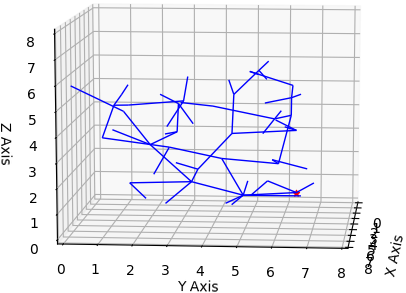
\includegraphics[width=0.45\linewidth]{chapters/chapter2/img/rrt_3d_1.png} & 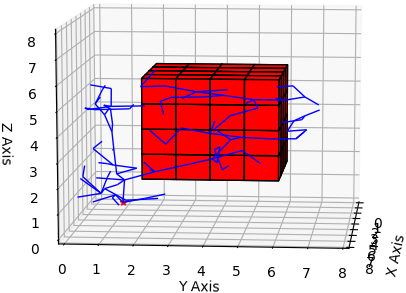
\includegraphics[width=0.45\linewidth]{chapters/chapter2/img/rrt_3d_2.png} \\
    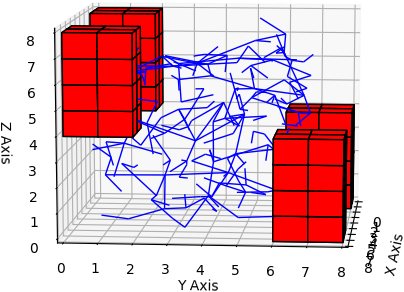
\includegraphics[width=0.45\linewidth]{chapters/chapter2/img/rrt_3d_3.png} & 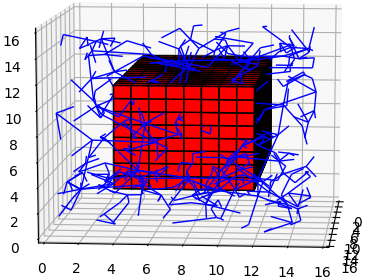
\includegraphics[width=0.45\linewidth]{chapters/chapter2/img/rrt_3d_4.png}
    \end{tabular}
    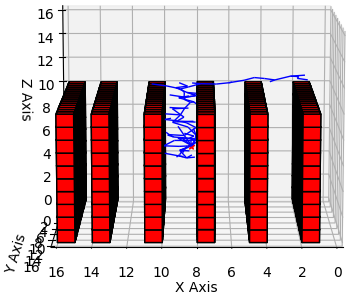
\includegraphics[width=0.45\linewidth]{chapters/chapter2/img/rrt_3d_5.png}
    \caption{3D RRT Implementation shown by \ac{GUI}}
    \label{figure:3DrrtGui}
\end{center}
\end{figure}


\newpage
\section{Analysis of RRT}
\label{section:rrt_analysis}
    % @Author: AnthonyKenny98
% @Date:   2020-02-28 15:02:19
% @Last Modified by:   AnthonyKenny98
% @Last Modified time: 2020-02-28 23:28:59

\todo[inline]{Brief introduction outlining purpose of performance analysis}

\subsection{Methodology}
    To restate, the aim of this thesis is to design a computer processor with reduced execution time of motion planning algorithms, such as \ac{RRT}. As such, it is important to understand the elements of the algorithm that have the highest percentage of CPU execution time. To determine this, it was necessary to implement my own, naive but typical, \ac{RRT} in C. This program could then be compiled and analysed using a software performance profiling tool. With this, I could design experiments to determine the critical RRT functions (those occupying a majority of CPU time) and see how this varies given different parameters.
    \todo[inline]{Outline of method of analysis. Something better than the above}

    \subsubsection{VTune Profiler}
    \label{subsubsection:vtune}
        VTune Profiler performance profiler is an application for software performance analysis. It provides functionality to examine hot-spots for CPU execution time through a top down analysis, shown below in Figure \ref{figure:VTuneTopDown}. As can be seen from the figure, the top down analysis tool shows the percentage of CPU time taken up by each function. I used this tool to profile the algorithm's performance as I changed certain parameters.
        \todo[inline]{Rewrite the above}
        % @Author: AnthonyKenny98
% @Date:   2020-02-23 14:33:19
% @Last Modified by:   AnthonyKenny98
% @Last Modified time: 2020-02-23 14:36:06

\begin{figure}[H]
\begin{center}
    \missingfigure[figwidth=\linewidth]{Screenshot of VTune Top Down Analysis (Maybe)}
    \caption{VTune Amplifier TopDown Analysis Example}
    \label{figure:VTuneTopDown}
\end{center}
\end{figure}

    \subsubsection{Internal Timing}
        The limitation of VTune Profiler is that it can only profile software running on Intel processors, which implement the x86-64 \ac{ISA}. As such, when the time comes to analyse performance of the software running on a RISC-V processor, another method will be required. A simple and effective way of measuring execution performance is to insert timing functionality into the software itself. 

    \subsubsection{Comparison}

\subsection{Results}
\label{section:rrt_analysis_results}

% Chapter 3
\chapter{Motion Planning in Hardware}
    \label{chap:MotionPlanningInHardware}
    % @Author: AnthonyKenny98
% @Date:   2020-02-26 08:22:07
% @Last Modified by:   AnthonyKenny98
% @Last Modified time: 2020-04-10 10:24:44

The second objective of this thesis was to design and implement a functional hardware unit that accelerates the execution of \gls{RRT} in \gls{3D}. With the bottleneck function having been identified in Chapter 2 as edge collision detection, Chapter 3 details the specification, design, implementation, and analysis of a hardware unit the implements the edge collision function.

\section{Defining the Collision Detection Unit}
    % @Author: AnthonyKenny98
% @Date:   2020-04-08 09:52:59
% @Last Modified by:   AnthonyKenny98
% @Last Modified time: 2020-04-10 15:07:12
\subsection{Edge Collision Function}
\label{subsection:EdgeCollisionFunction}
    To briefly examine the edge collision detection function in general terms; Given an edge $e$, \gls{RRT} finds where $e$ intersects with grids in the \gls{OGM}. If any of the grids intersected are ``occupied'', a collision is returned. This is shown in Figure \ref{fig:edge_collision_process} on Page \pageref{fig:edge_collision_process}. 

    Calculating intersections between a segment and grids is very computationally intense. This is because it is a fairly involved geometric process. Figure \ref{fig:edge_collision_planes} on Page \pageref{fig:edge_collision_planes} shows how grid intersections are detected by computing the point at which the segment intersects certain \textbf{\glspl{axis-oriented plane}}.  

    \subsubsection{Time Complexity}
        With the steps of the edge collision algorithm understood (explained graphically in Figure \ref{fig:edge_collision_planes}, algorithm included in Appendix \ref{section:rrt_appendix_function_impl}), its \gls{time complexity} may be quantified. 
        For an edge $e$ of maximum length $\epsilon$, it must check for intersections with $\epsilon \times \epsilon \times \epsilon$ grids. (i.e the only grids that are checked are the ones that the $e$ could possibly intersect with). 
        It first iterates through the three dimensions of \glspl{axis-oriented plane} ($xy$, $xz$, and $yz$). This is a constant of 3. 
        Within each of these dimensions, it must iterate through $\epsilon$ planes. This makes its time complexity $O(3\epsilon)$. 

        % @Author: AnthonyKenny98
% @Date:   2020-04-07 11:00:50
% @Last Modified by:   AnthonyKenny98
% @Last Modified time: 2020-04-07 12:40:47
\begin{figure}[H]
\begin{centering}
\begin{tabular}{cc}
    \begin{subfigure}{0.47\linewidth}
    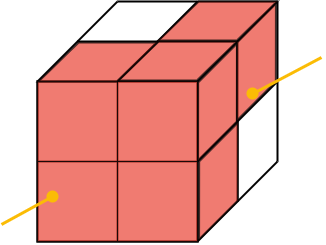
\includegraphics[width=\linewidth]{chapters/chapter3/img/edge_collision_planes_a.png}
    \caption{}
    \label{fig:edge_collision_planes_a}
    \end{subfigure} &

    \begin{subfigure}{0.47\linewidth}
    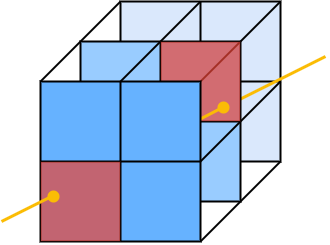
\includegraphics[width=\linewidth]{chapters/chapter3/img/edge_collision_planes_b.png}
    \caption{}
    \label{fig:edge_collision_planes_b}
    \end{subfigure} \\

    \begin{subfigure}{0.47\linewidth}
    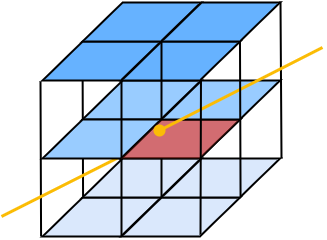
\includegraphics[width=\linewidth]{chapters/chapter3/img/edge_collision_planes_c.png}
    \caption{}
    \label{fig:edge_collision_planes_c}
    \end{subfigure} &

    \begin{subfigure}{0.47\linewidth}
    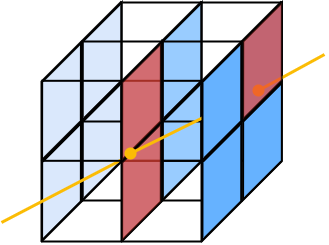
\includegraphics[width=\linewidth]{chapters/chapter3/img/edge_collision_planes_d.png}
    \caption{}
    \label{fig:edge_collision_planes_d}
    \end{subfigure} \\
\end{tabular}

\mycaption{Detecting Grid Intersections by Finding Intersections with Axis Oriented Planes}{\\ Consider an edge $e$ that spans the width of a $2\times 2\times 2$ grid map, as shown in Figure \ref{fig:edge_collision_planes} (do not consider if the grids are occupied, this is just to determine which of them the edge intersects). Just by eyeballing Figure \ref{fig:edge_collision_planes_a} it seems odd that so many of the grids have been intersected (denoted by red shading) by the yellow edge. The algorithm executed by checking one set of \glspl{axis-oriented plane} at a time. Figure \ref{fig:edge_collision_planes_a} shows how the $xy$-oriented planes are checked for 3 different values of $z$ (going into the page), finding two intersection points. There is only one intersection for the $xz$ oriented planes (\ref{fig:edge_collision_planes_c}). In Figure \ref{fig:edge_collision_planes_d}, the segment intersects 2 grids in the second $yz$-oriented plane, and one in the third plane. The intersected grids are thus any grid where a point-of-intersection falls on its face.}
\label{fig:edge_collision_planes}
\end{centering}
\end{figure}

        % @Author: AnthonyKenny98
% @Date:   2020-04-06 17:52:43
% @Last Modified by:   AnthonyKenny98
% @Last Modified time: 2020-04-06 17:52:43

   
\subsection{Technical Specifications}
\label{subsection:HoneyBeeSpecs}

    \subsubsection{Performance Specifications}
        When accelerating motion planning algorithms, it is often difficult to quantify a goal for how much faster one would like the function to run - the answer is usually ``as fast as possible!'' For this thesis, the performance specification was set that the edge collision function run fast enough that it was no longer the bottleneck function. This translated to a desired speedup of about 3 times (when compared to benchmark performance of a typical CPU). Table \ref{table:edg_col_performance_specs} quantifies this in terms of latency and throughput.

        % @Author: AnthonyKenny98
% @Date:   2020-04-07 13:28:39
% @Last Modified by:   AnthonyKenny98
% @Last Modified time: 2020-04-08 16:26:52
\begin{table}[H]
\begin{centering}
\begin{tabular}{|c|c|c|}
\hline
\textbf{Metric}     &   \textbf{Benchmark CPU$^*$}   & \textbf{Accelerated} \\
\hline
Latency ($\mu$seconds/edge)  &   2.6  & 0.9 \\
\hline
Throughput (edges/second)  &   384,615  & 1,111,111 \\
\hline
\end{tabular}
\mycaption{Performance Specifications for Edge Collision Detection Unit}{. $^*$Benchmark CPU is an Intel 3.1 GHz i7 Dual Core processor, typical of a laptop computer.}
\label{table:edg_col_performance_specs}
\end{centering}
\end{table}

\newpage

\subsubsection{Area Specifications}
    Generally, an inverse relationship exists between latency and area. While it may be possible to make the unit much faster than the latency specification, this may become prohibitive with regards to the amount of area on chip it would occupy. It was decided to limit the area to that which would fit on an \gls{FPGA} typical in drone applications (those of the Kintex-7 Low Voltage family were chosen, but there are many possible options). 

    Logic area on an FPGA is largely determined by \glspl{LUT}. \glsdesc{LUT_g} As such, the upper bound on area was set at 274,080 \glspl{LUT}.

\subsubsection{Interface Specifications}
\label{subsection:HoneyBeeTechSpechs}
    As shown in Figure \ref{fig:edge_collision_process}, the computationally intensive part of the process of edge collision detection is finding points of intersection between an edge and the grids of the map. Comparing this result to an \gls{OGM} is simple and fast. Therefore, it was decided that the hardware unit would simply take an edge and determine the grids with which it intersects. Whether the edge intersects a given grid can be represented as a binary $\{0,1\}$, and thus the intersections found in a $\epsilon \times \epsilon\times\epsilon$ gridspace can be represented as an $\epsilon^3$ sequence of binary values.
    Table \ref{table:edg_col_interface_specs} outlines the required interface specifications for the functional unit.
    % @Author: AnthonyKenny98
% @Date:   2020-03-01 14:11:33
% @Last Modified by:   AnthonyKenny98
% @Last Modified time: 2020-04-07 14:09:51
\begin{table}[H]
\begin{center}
\begin{tabular}{|p{.2\linewidth}|p{.74\linewidth}|}
    \hline
    \textbf{Element}             & \textbf{Description/Justification} \\
    \hline
    \multicolumn{2}{|c|}{Constraints} \\
    \hline
    Length $\epsilon$  & $\epsilon$ defines the max edge length. The space being checked and the output sequence has the dimensions $\epsilon\times\epsilon\times\epsilon$ \\
    \hline
    \multicolumn{2}{|c|}{Inputs} \\
    \hline
    Edge $e$  & An Edge $e$ defined for a \gls{3D} \gls{configuration} space by two points $\{p1, p2\}$, each defined by a set of \gls{3D} coordinates $\{x,y,z\}$.\\
    \hline
    Control Inputs & The functional unit must have ports for control signals: clock, reset, start. These are required for adding the unit to a processor. \\
    \hline
    \multicolumn{2}{|c|}{Outputs} \\ 
    \hline
    Return Value & $\epsilon^3$ bit sequence: 1 if collides with grid at that index, 0 otherwise.\\
    \hline
    Control Outputs & Output ports for control signals: idle, done, ready. These are required for adding the unit to a processor. \\
    \hline
\end{tabular}
\mycaption{Interface Specifications for Edge Collision Detection Unit}{}
\label{table:edg_col_interface_specs}
\end{center}
\end{table}

\newpage

\section{HoneyBee}
    % @Author: AnthonyKenny98
% @Date:   2020-04-08 09:56:57
% @Last Modified by:   AnthonyKenny98
% @Last Modified time: 2020-04-09 07:02:40

% @Author: AnthonyKenny98
% @Date:   2020-04-06 17:19:39
% @Last Modified by:   AnthonyKenny98
% @Last Modified time: 2020-04-06 17:29:38
\begin{figure}[H]
\begin{centering}
\includegraphics[width=0.8\linewidth]{chapters/chapter3/img/MegalongHoneyBee.png}
\mycaption{Megalong Park Honey Bee Pollinating a Weeping Cherry Blossom}{. Photographed by Emma Kenny in the Southern Highlands of New South Wales, Australia}
\end{centering}
\end{figure}

The honey bee, \textit{Apis mellifera}, has long been renowned for its tireless work ethic. However, the it is rarely given credit for its remarkable navigation and collision avoidance strategies during flight. Recent research\cite{Menzel2005} suggests that honey bees, interestingly enough, explore their workspace randomly in order to find paths from their hive to sources of pollen. Sound familiar? As such, it is quite appropriate that this functional unit, designed to work tirelessly, rapidly and efficiently to execute collision detection computations for robot motion planning, was named \textbf{HoneyBee}. \\
\bigskip

HoneyBee is a hardware unit that will eventually be incorporated into a processor, demonstrated in Figure \ref{fig:honeybee_in_processor}. In Chapter 4, the HoneyBee unit is implemented in a simple RISC-V processor and invoked using custom RISC-V instructions. For now, however, consider HoneyBee as a standalone unit that computes the grids with which an edge collides. Its resulting output can be compared to an \gls{OGM}, as explained in section \ref{subsection:EdgeCollisionFunction}.

% @Author: AnthonyKenny98
% @Date:   2020-04-08 11:15:41
% @Last Modified by:   AnthonyKenny98
% @Last Modified time: 2020-04-08 11:20:08
\begin{figure}[H]
\begin{centering}
% \includegraphics[width=\linewidth]{name}
\missingfigure[figwidth=\linewidth]{HoneyBee in a Processor}
\caption{}
\label{fig:honeybee_in_processor}
\end{centering}
\end{figure}

\subsection{HoneyBee Interface Design}
    The interface for the HoneyBee functional unit, following on from the interface specifications outlines in Section \ref{subsection:HoneyBeeTechSpechs} can be simply represented by Figure \ref{fig:honeybee_interface_simple}.

    % @Author: AnthonyKenny98
% @Date:   2020-04-08 10:23:56
% @Last Modified by:   AnthonyKenny98
% @Last Modified time: 2020-04-08 10:44:54
\begin{figure}[H]
\begin{centering}

\includegraphics[width=0.6\linewidth]{chapters/chapter3/img/honeybee_interface_simple.png}
\mycaption{General Overview of HoneyBee Interface}{. The functional unit takes an edge $e$, defined by two points $p_1$ and $p_2$, as an input, and outputs a series of collisions. These collisions describe which grids an edge intersects. Its control interface allows for communication with a processors main control unit.}
\label{fig:honeybee_interface_simple}
\end{centering}
\end{figure}
    
    However, when designing hardware (the method of doing so is described in section \ref{section:honeybee_implementation}), how these inputs and outputs are implemented must be considered at the \gls{bit} level. Figure \ref{fig:honeybee_interface_detail} shows all input, output, and control ports, and their \glspl{bit-width}. 
    
    % @Author: AnthonyKenny98
% @Date:   2020-04-08 10:33:04
% @Last Modified by:   AnthonyKenny98
% @Last Modified time: 2020-04-08 11:30:28
\begin{figure}[H]
\begin{centering}
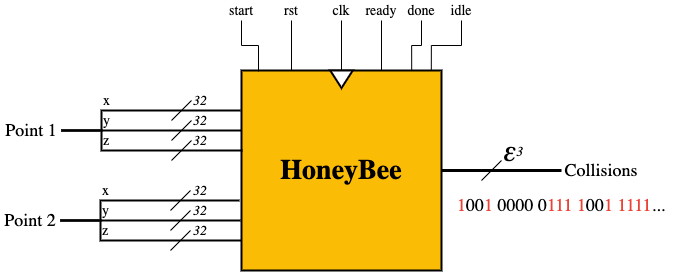
\includegraphics[width=0.8\linewidth]{chapters/chapter3/img/honeybee_interface_detail.png}
\mycaption{Port Diagram of HoneyBee Interface}{. The edge input is represented by 6 32-bit floats, following the IEEE 754 Single Precision 32-bit protocol, each float representing one of its coordinate points. The output sequence of collisions is a $e^3$-bit sequence, with each bit in the sequence representing one of the grids that was checked for intersections. It has input control signals for start and reset, and output control signals for done, idle, and ready. These control signals make up the necessary signals for a handshake protocol between HoneyBee and a processor's main controller.}
\label{fig:honeybee_interface_detail}
\end{centering}
\end{figure}

    \subsubsection{Inputs}
        The inputs to HoneyBee collectively describe a single edge. This is done with 6 32-bit floating point numbers. How floating points (non-integer numbers) are represented in binary determined by the \gls{IEEE754}. How this is actually represented is not neccesary to understand, but is explained in Appendix \ref{section:honeybee_appendix_ieee}. The important point is that the input edge determined by 6 32-bit coordinate points.

    \subsubsection{Output}
        HoneyBee outputs a sequence of ``collision-bits,'' with each bit in the sequence representing if the input edge collides with its corresponding bit. How this sequence of bits is mapped to a \gls{3D} grid-map is explained in Appendix \ref{section:honeybee_appendix_mapping}. It is important to note that in the design and implementation of HoneyBee, the length of this sequence was parameterized to be variable, corresponding to a variable value of $\epsilon$. Recall that the optimal edge collision algorithm only checked $\epsilon^3$ grids. HoneyBee, as well, only checks the grids with which the edge could possible intersect.

        Since the number of grids being checked is parameterized, so must the number of collision-bits be. This is demonstrated in Figure \ref{section:honeybee_epsilon_grids}.
        % @Author: AnthonyKenny98
% @Date:   2020-04-08 11:48:44
% @Last Modified by:   AnthonyKenny98
% @Last Modified time: 2020-04-08 11:54:02
\begin{figure}
\begin{centering}
\begin{tabular}{c c}

    \begin{subfigure}{0.4\linewidth}
    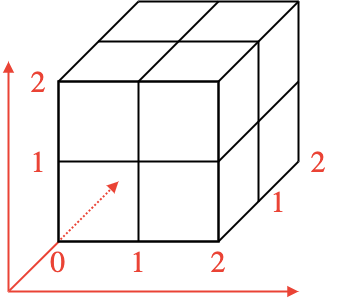
\includegraphics[width=\linewidth]{chapters/chapter3/img/honeybee_epsilon_grids_a.png}
    \caption{For $\epsilon=2$, an output collision-bit sequence of length 8 is required.}
    \end{subfigure} & 

    \begin{subfigure}{0.4\linewidth}
    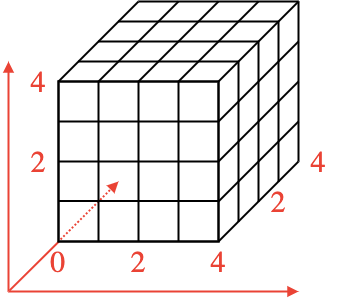
\includegraphics[width=\linewidth]{chapters/chapter3/img/honeybee_epsilon_grids_b.png}
    \caption{For $\epsilon=4$, an output collision-bit sequence of length 64 is required.}
    \end{subfigure} \\    

\end{tabular}
\mycaption{The Impact of $\epsilon$ on the Length of the Bit-Collision Sequence}{}
\label{fig:honeybee_epsilon_grids}
\end{centering}
\end{figure}

        \textbf{Note:} The output \gls{bit-width} is \textit{parameterized} not \textit{variable}. Upon synthesis (building) of HoneyBee, the output \gls{bit-width} is set at a constant value. Different syntheses may have different output \glspl{bit-width}. When the time comes to add HoneyBee to a processor, it is synthesized with a certain \gls{bit-width}.

    \subsubsection{Control Interface}
        The control interface is designed to give HoneyBee the ability to be included in a processor, and implements a commonly used ``handshake'' protocol between HoneyBee and the control unit of the processor in which it resides. Put simply, this is a method that allows the control unit to tell HoneyBee when to start executing the computation, and for HoneyBee to tell the control unit when it has finished its computation and the output value is ready. This is explained in detail in Appendix \ref{section:honeybee_appendix_handshake}. The control interface also has a clock and reset port.


\subsection{HoneyBee Implementation}
\label{section:honeybee_implementation}
    \subsubsection{Hardware Description Languages}
        Designing computers and their constituent parts has come a long way from its arduous beginnings. ``Victory'', the enigma-breaking machine designed by Alan Turing at Bletchley Park during World War II, was a large electro-mechanical computer made up of storage wheels, electromagnetic relays, and rotary switches, assembled by hand.\cite{ChoiceReviews2006} So too was ``Mark I'', the 816 cubic feet computer designed by Harvard University's Dr. Howard Aiken, which, on March 1944, computed the viability of implosion for detonating the atomic bomb.\cite{Elsabbagh2019}
        
        % @Author: AnthonyKenny98
% @Date:   2020-04-08 13:30:24
% @Last Modified by:   AnthonyKenny98
% @Last Modified time: 2020-04-08 13:54:06
\begin{figure}
\begin{centering}
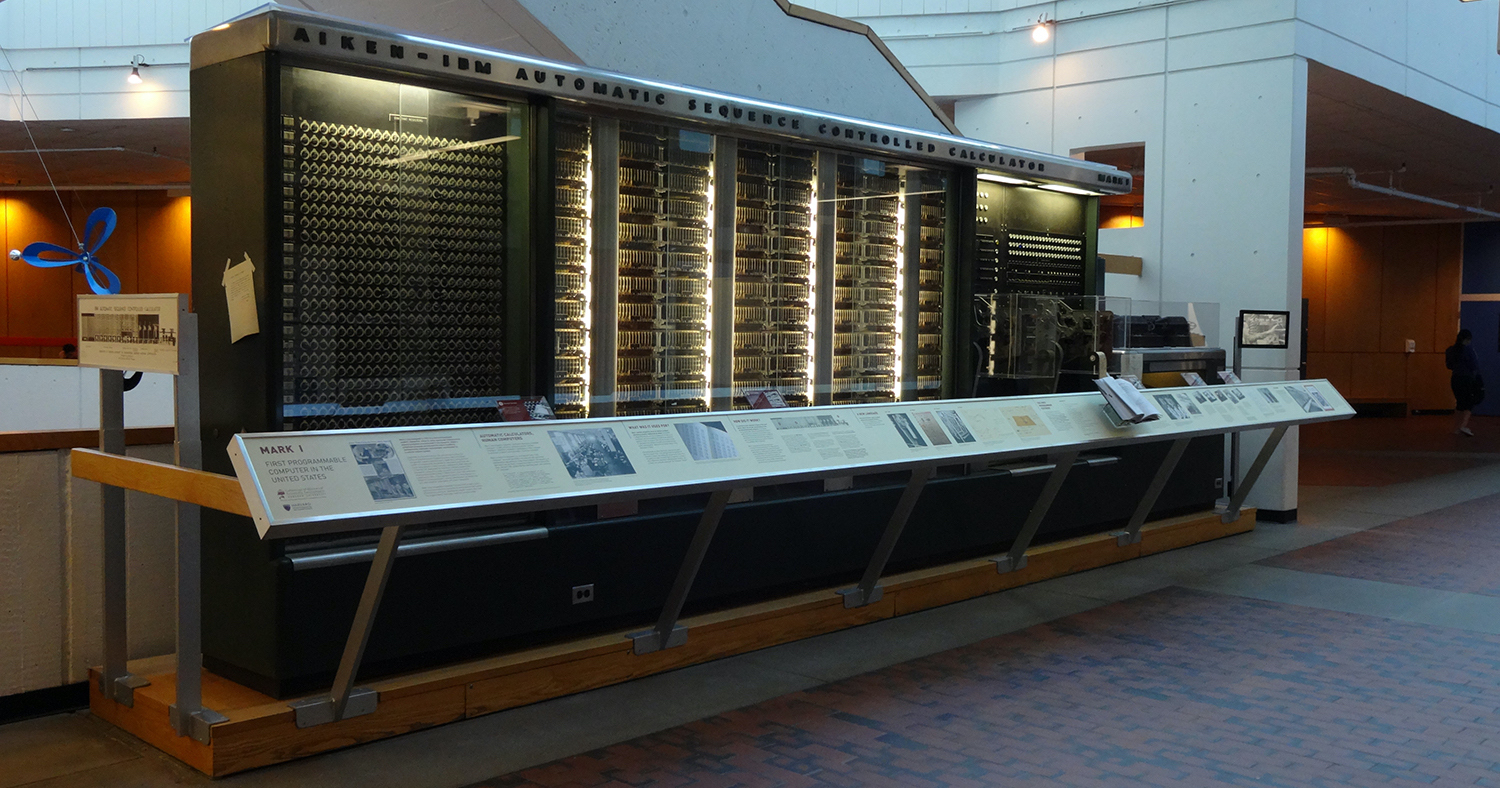
\includegraphics[width=0.7\linewidth]{chapters/chapter3/img/mark1.jpeg}
\mycaption{The Harvard Mark I Computer}{, photographed in the Harvard Science Center in April 2014 (Source: Harvard University)}
\end{centering}
\end{figure}

        Computers nowadays measure in the order of millimeters rather than meters. What's more, they are now ``built'' in software, using a \glsfirst{HDL}. \glspl{HDL} is a family of computer programming languages that are used to specify the function of electronic circuits. Tools allow for simulation of such circuits to verify design correctness and performance. Modules defined in \glspl{HDL} may then be synthesized for a type of integrated circuit called a \glsfirst{FPGA}. This \gls{FPGA}, ``programmed'' in \gls{HDL} code to behave in a certain way, can then serve the purpose of a processor or other functional processing unit. Figure \ref{fig:hdl_to_fpga} demonstrates this process.

        % @Author: AnthonyKenny98
% @Date:   2020-04-08 13:37:54
% @Last Modified by:   AnthonyKenny98
% @Last Modified time: 2020-04-08 14:00:57
\begin{figure}[H]
\begin{centering}
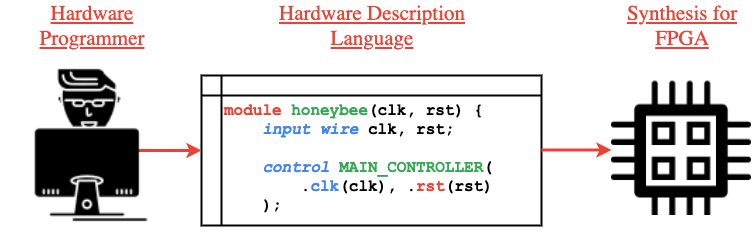
\includegraphics[width=\linewidth]{chapters/chapter3/img/hdl_to_fpga.png}
\mycaption{The Hardware Development Process}{, Defining Hardware Units in Hardware Description Languages for FPGAs.}
\end{centering}
\end{figure}

        HoneyBee was implemented eventually in an \gls{HDL} called Verilog. However, no Verilog for HoneyBee was ever explicitly written by a human. It was generated by a tool called High-Level Synthesis.

    \subsubsection{High Level Synthesis}
        \gls{HLS} is an automated hardware design process that takes design files (written in high-level languages, such as C, C++ or SystemC) specifying the algorithmic function of a piece of hardware, interprets those files, and creates digital hardware designs that execute this function. In short, it effectively translates programming languages into hardware description languages. Some key advantages of using HLS are speed and verification. It is much faster and easier to define functionality in C than it is in a \gls{HDL} such as Verilog, and thus design iterations are faster. It is also much simpler to verify one's design, as the functional units can be put through test benches written in C. \\

        The most important benefit of using \gls{HLS}, however, is the ability to use ``pragmas.'' These are simply directives given to the \gls{HLS} tool that tell it what optimizations to use when translating C code into an \gls{HDL}. This allows the same funtionality to be synthesized in many different ways, optimizing the synthesis for speed, area, memory, etc. As such, the hardware development process now allows developers to experiment quickly with different ways to implement the same functionality. This is demonstrated graphically by Figure \ref{fig:hls_to_fpga} on Page \pageref{fig:hls_to_fpga}.

        % @Author: AnthonyKenny98
% @Date:   2020-04-08 15:17:43
% @Last Modified by:   AnthonyKenny98
% @Last Modified time: 2020-04-08 16:02:17
\begin{figure}
\begin{centering}
\begin{tabular}{c}

\begin{subfigure}{0.97\linewidth}
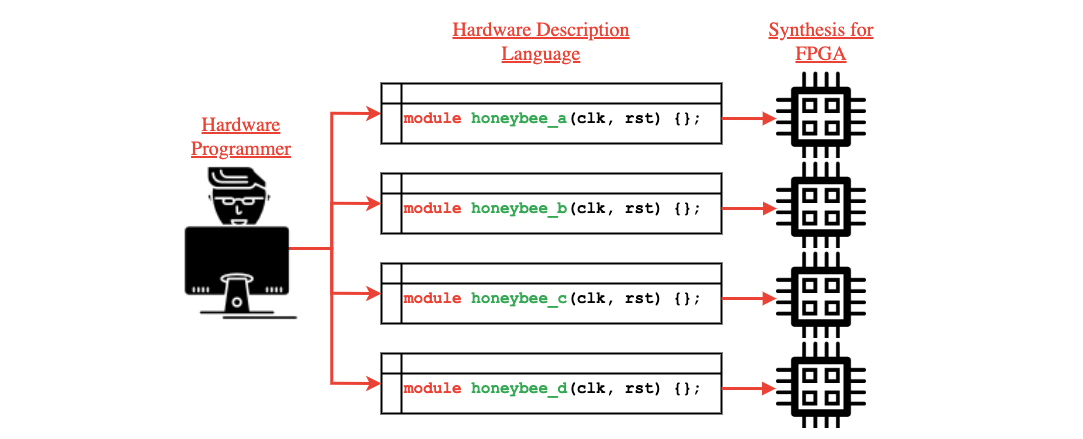
\includegraphics[width=\linewidth]{chapters/chapter3/img/hls_to_fpga_a.png}
\caption{Hardware Optimization without HLS}
\label{fig:hls_to_fpga_a}
\end{subfigure} \\

\begin{subfigure}{0.97\linewidth}
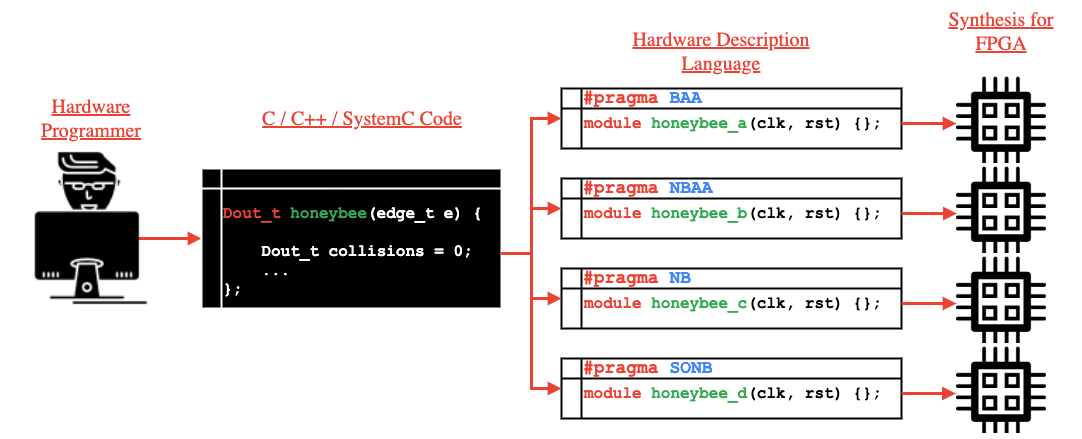
\includegraphics[width=\linewidth]{chapters/chapter3/img/hls_to_fpga_b.png}
\caption{Hardware Optimization with HLS}
\label{fig:hls_to_fpga_b}
\end{subfigure}

\end{tabular}
\mycaption{Hardware Optimization Process}{. Figure \ref{fig:hls_to_fpga_a} shows how, without using HLS, the hardware developer must write multiple different implementation of the same functionality to acheive different performance. Figure \ref{fig:hls_to_fpga_b} shows how, when using HLS, the hardware developer only must write one implementation (in a higher-level language like C), and then use ``pragmas'' to create different implementations (with different optimizations) for synthesis.}
\label{fig:hls_to_fpga}
\end{centering}
\end{figure}

    \subsubsection{HoneyBee-A Synthesis}
        With the functionality of HoneyBee implemented in C, the first optimization iteration (designated \gls{HB-A}) was synthesized. \gls{HB-A} had no pragmas, and was merely a basic hardware implementation of the defined functionality. \gls{HB-A} and all subsequent iterations) synthesized correctly to the interface specifications (See Appendix \ref{section:honeybee_appendix_synthesis_report} for technical interface report of synthesis). Table \ref{table:HBA_results} shows the result of \gls{HB-A}'s synthesis compared with its performance and area specifications. Obviously, the synthesis is well below the area limit, but nowhere near the specifed performance metrics. This is where the beauty of High-Level Synthesis optimization came in.

        % @Author: AnthonyKenny98
% @Date:   2020-04-08 15:34:16
% @Last Modified by:   AnthonyKenny98
% @Last Modified time: 2020-04-08 15:49:09
\begin{table}[H]
\begin{center}
\begin{tabular}{|c|c|c|}
    \hline
    \textbf{Metric}             & \textbf{Specification} & \textbf{Synthesis Result} \\
    \hline
    Latency ($\mu$seconds/edge)  &   0.9  & \textcolor{myred}{6.66} \\
    \hline
    Throughput (edges/second)  &   1,111,111 & \textcolor{myred}{150,150} \\
    \hline
    FPGA Area \glspl{LUT} & 274,080  & \textcolor{mygreen}{10,593} \\
    \hline
\end{tabular}
\mycaption{Synthesis Results for HB-A with $\epsilon = 4$}{}
\label{table:HBA_results}
\end{center}
\end{table}

\newpage
\subsection{HoneyBee Acceleration}
    This section steps through the process of using \gls{HLS} \glspl{pragma} in 2 major optimization iterations, \gls{HB-B} and \gls{HB-C} and how these iterations compared to benchmark and specified performance.

    \subsubsection{Benchmarking}
        The benchmark performance was based on a Dual-Core Intel 3.1GHz i7 processor. In an ideal world, this processor would have been chosen after a rigourous process of determining the most suitable benchmark. In reality, this processor was chosen because it was the one found in the computer running the simulations (an early 2015 MacBook Pro). Nevertheless, it serves as a suitable benchmark, demonstrating performance typical of general purpose CPUs.

        Examining latency, the benchmark was set at the average execution time for the benchmark CPU to compute 1 edge. Tests were run and averaged over 1000 trials. The average latency was 2.6 $\mu$seconds, with a standard deviation of 0.1 $\mu$seconds. This is shown, along with the performance of \gls{HB-A} in Figure \ref{fig:benchmark_1}.

        % @Author: AnthonyKenny98
% @Date:   2020-04-08 16:42:38
% @Last Modified by:   AnthonyKenny98
% @Last Modified time: 2020-04-08 17:12:56
\begin{figure}[H]
\begin{centering}
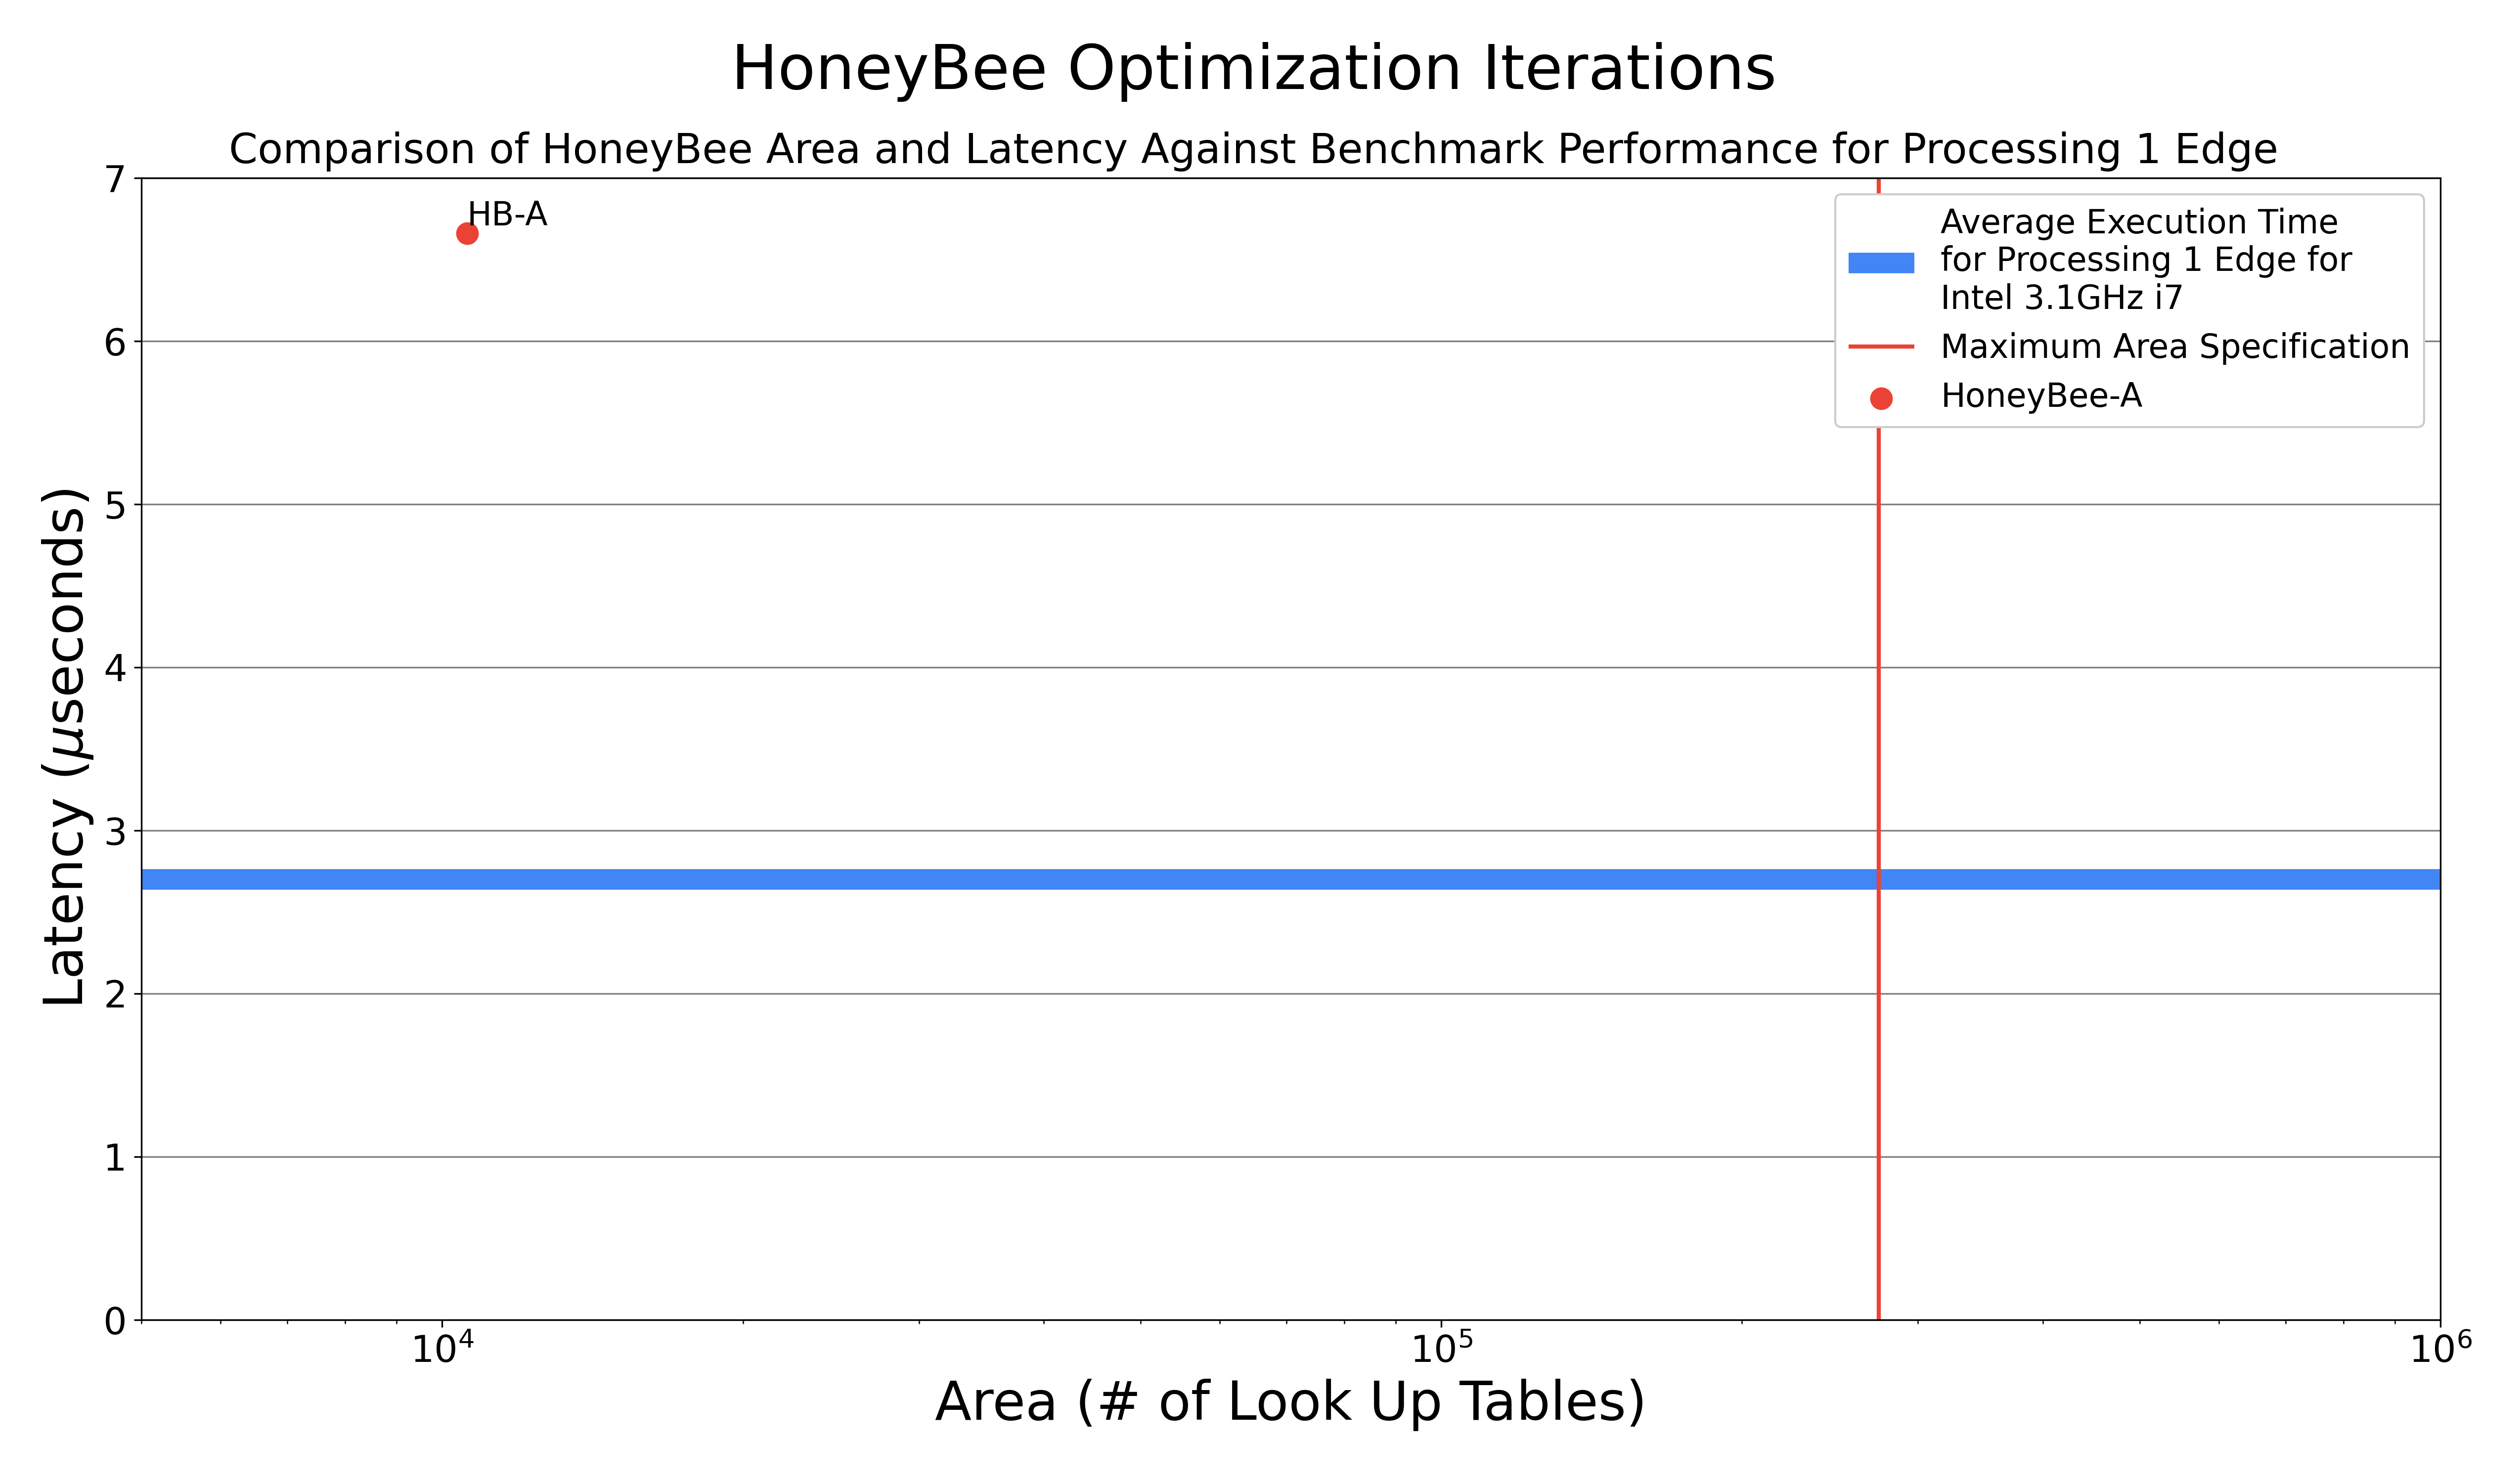
\includegraphics[width=\linewidth]{chapters/chapter3/img/benchmark_1.png}
\mycaption{HB-A Performance Against Benchmark CPU}{. Standard deviation of CPU average performance is shown by width of the line for easier interpretation.}
\label{fig:benchmark_1}
\end{centering}
\end{figure}

    \subsubsection{HoneyBee-B}
        The first step in accelerating HoneyBee was taking advantage of the inherent parrallelism available to the algorithm. Recall that the edge collision algorithm checks the $xy$-oriented planes, the $xz$-oriented planes, and finally the $yz$-oriented planes. These operations are completely independent, and can thus be performed simultaneously. Figure \ref{fig:hbb_timing} shows how the process of checking each set of planes was done sequentially in \gls{HB-A}, but are executed in parallel in \gls{HB-B}.

        % @Author: AnthonyKenny98
% @Date:   2020-04-08 18:12:53
% @Last Modified by:   AnthonyKenny98
% @Last Modified time: 2020-04-10 15:20:20
\begin{figure}[H]
\begin{centering}
\begin{tabular}{c}

\begin{subfigure}{0.97\textwidth}
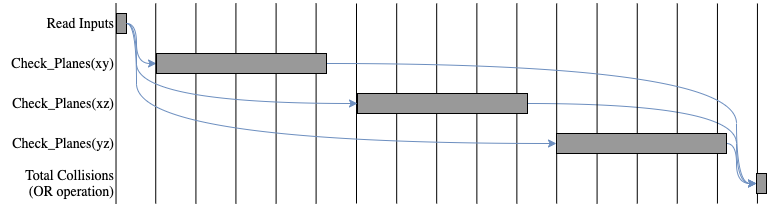
\includegraphics[width=\linewidth]{chapters/chapter3/img/timing1.png}
\caption{HoneyBee-A Timing Diagram. \texttt{Check\_Planes} executed sequentially.}
\label{fig:hbb_timing_a}
\end{subfigure} \\

\begin{subfigure}{0.97\textwidth}
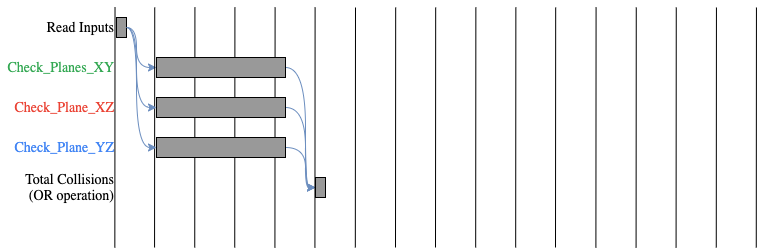
\includegraphics[width=\linewidth]{chapters/chapter3/img/timing2.png}
\caption{HoneyBee-B Timing Diagram. \texttt{Check\_Planes} executed in parallel. Different colors are to represent slightly different implementations of the same function.}
\label{fig:hbb_timing_b}
\end{subfigure} \\

\end{tabular}
\mycaption{Timing Diagrams Showing Parallelization in HoneyBee-B}{. Note, these are simlified timing diagrams for easy explanation of the concept of hardware parallelization.}
\label{fig:hbb_timing}
\end{centering}
\end{figure}

        The timing diagram does not only show the use of parallelism. It also shows how this is actually implemented in hardware. In \gls{HB-A} (Figure \ref{fig:hbb_timing_a}), there is a single module named \texttt{Check\_Plane}. Since there is only one of them, it must calculate intersections with each set of planes sequentially. On the other hand, in \gls{HB-B} (Figure \ref{fig:hbb_timing_b}), there are three seperate instances of this module (\texttt{Check\_Planes\_XY}, \texttt{Check\_Planes\_XZ}, and \texttt{Check\_Planes\_YZ}), allowing HoneyBee to execute computation on all three sets of planes in parallel. 

        Moreover, notice that in \gls{HB-B}, execution time of each of these three instances is shorter than that of the single instance in \gls{HB-A}. When a single module instance is used for different purposes (in this case, checking the $xy$, $xz$, and $yz$ oriented planes), it has some variability. To control this variability, it must execute a certain amount of control logic at the beginning of the function. On the other hand, when there are seperate instances of the module, what was once variable can now be made constant. As a result, each instance can be slightly specialized and the control logic eliminated. In this case, a general \texttt{Check\_Planes} module was replaced with the three specialized \texttt{Check\_Planes\_XY}, \texttt{Check\_Planes\_XZ}, and \texttt{Check\_Planes\_YZ}. Each of these has less variability, thus less control logic, and therefore a slightly faster overall latency. Figure \ref{fig:hbb_timing} shows how theoretically, this should result in a reduction in overall latency of more than 3 times.\\

        Comparing HoneyBee-B against our benchmark, the success of this optimization can be seen. Figure \ref{fig:benchmark_2} shows the performance of multiple variants of \gls{HB-B} in yellow. These variants were the result of experimenting with slightly different \glspl{pragma}, but all fell in roughly the same area. Appendix \ref{section:honeybee_appendix_hbb_variants} lists the details of each \gls{HB-B} variant. \\
        HB-B3 showed the best performance/area relationship. It was of acceptable area and had latency marginally lower than the benchmark, but was not as fast as the defined specifications. Table \ref{table:HBB_results} shows the result of HB-B3's synthesis compared with its performance and area specifications.

        % @Author: AnthonyKenny98
% @Date:   2020-04-08 15:34:16
% @Last Modified by:   AnthonyKenny98
% @Last Modified time: 2020-04-08 19:38:23
\begin{table}[H]
\begin{center}
\begin{tabular}{|c|c|c|}
    \hline
    \textbf{Metric}             & \textbf{Specification} & \textbf{Synthesis Result} \\
    \hline
    Latency ($\mu$seconds/edge)  &   0.9  & \textcolor{myred}{2.05} \\
    \hline
    Throughput (edges/second)  &   1,111,111 & \textcolor{myred}{487,805} \\
    \hline
    FPGA Area \glspl{LUT} & 274,080  & \textcolor{mygreen}{26,524} \\
    \hline
\end{tabular}
\mycaption{Synthesis Results for HB-B3 with $\epsilon = 4$}{}
\label{table:HBB_results}
\end{center}
\end{table}

        % @Author: AnthonyKenny98
% @Date:   2020-04-08 17:54:49
% @Last Modified by:   AnthonyKenny98
% @Last Modified time: 2020-04-08 19:08:39
\begin{figure}[H]
\begin{centering}
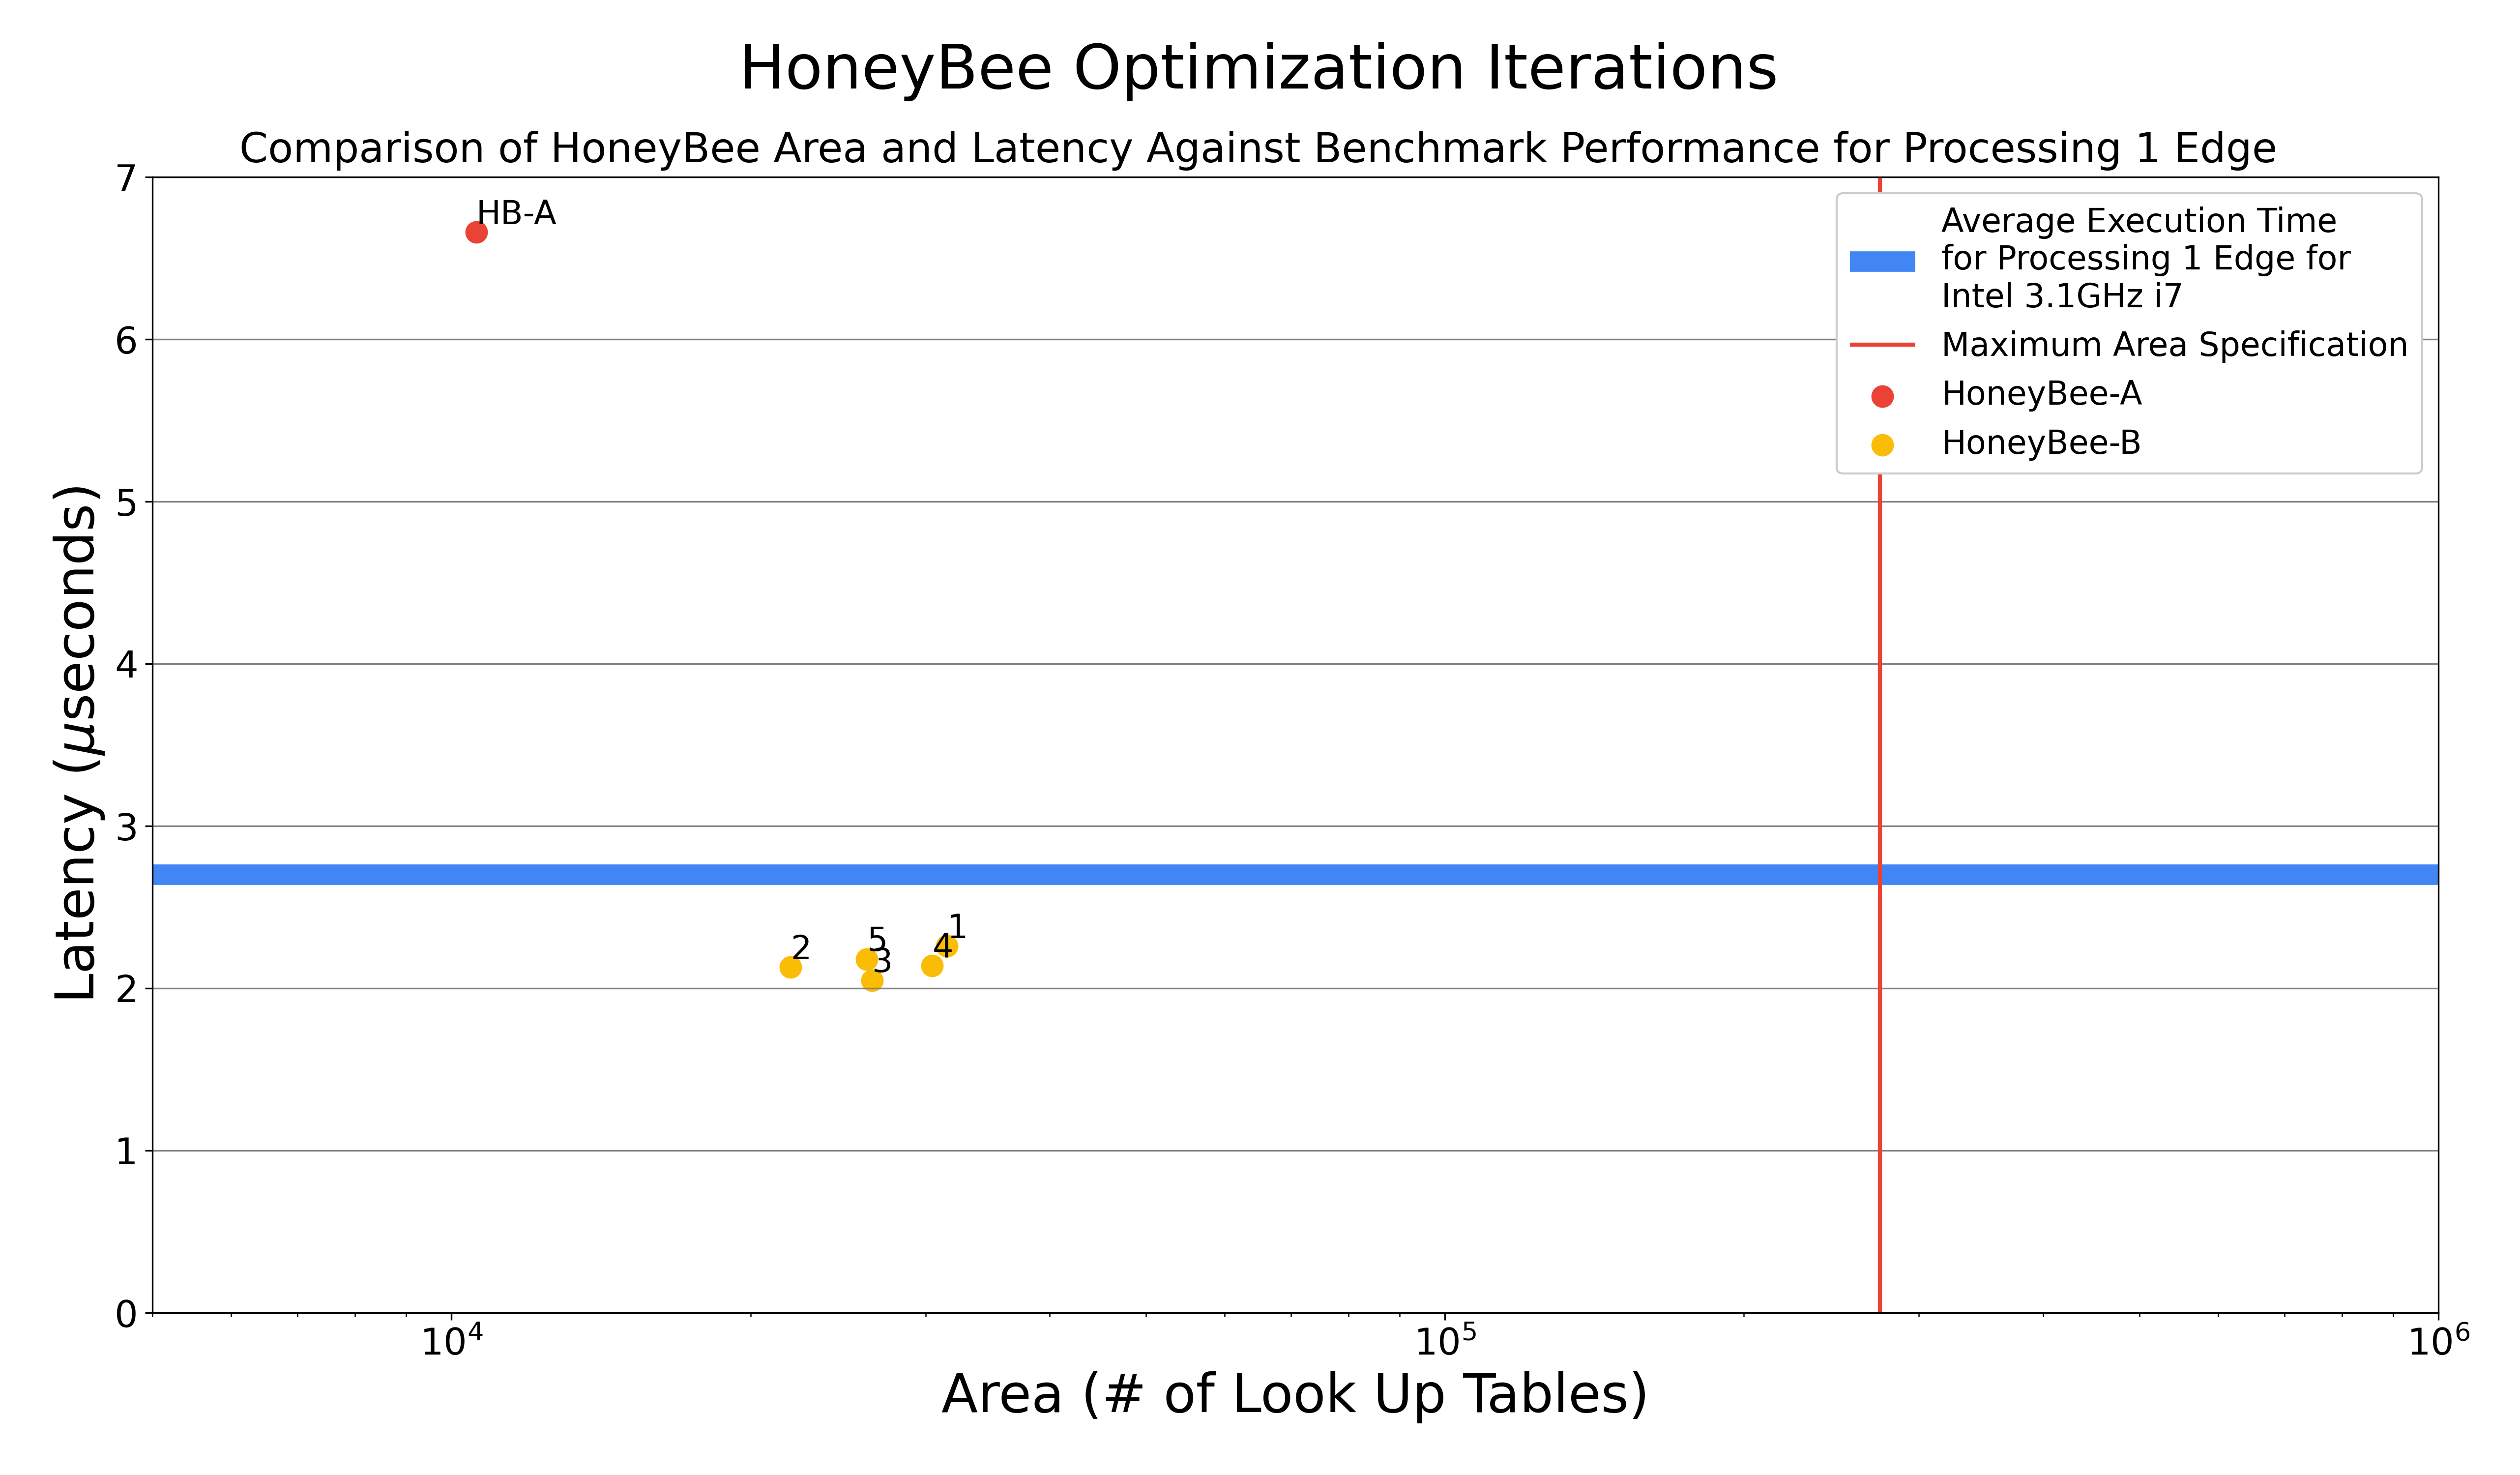
\includegraphics[width=\linewidth]{chapters/chapter3/img/benchmark_2.png}
\mycaption{HB-B Performance Against Benchmark CPU}{\\ Variants of HB-B shown in Yellow.}
\label{fig:benchmark_2}
\end{centering}
\end{figure}

    \subsubsection{HoneyBee-C}
        A similar concept was applied to optimize the computation of each set of planes. Consider synthesis of HoneyBee for $\epsilon = 4$. HoneyBee will need to compute intersections with 4 $xy$-oriented planes, 4 $xz$-oriented planes, and 4 $yz$-oriented planes. \gls{HB-B} computes each set of 4 planes simultaneously, but the computing intersections with each of the 4 planes in one orientation are also independent operations. As such, they can also be parallelized with the instantiation of more hardware modules. Figure \ref{fig:hbc_timing} shows the timing diagrams for the \texttt{Check\_Planes\_XY} module that was shown in the last set of timing diagrams.

        % @Author: AnthonyKenny98
% @Date:   2020-04-08 18:12:53
% @Last Modified by:   AnthonyKenny98
% @Last Modified time: 2020-04-08 19:21:39
\begin{figure}[H]
\begin{centering}
\begin{tabular}{c}

\begin{subfigure}{\linewidth}
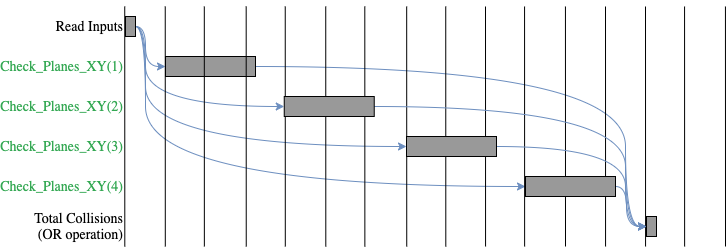
\includegraphics[width=\linewidth]{chapters/chapter3/img/timing3.png}
\caption{HoneyBee-B Timing Diagram for \texttt{Check\_Planes\_XY}. One instance of \texttt{Check\_Planes\_XY} module executed sequentially 4 times ($\epsilon=4$.}
\label{fig:hbb_timing_a}
\end{subfigure} \\

\begin{subfigure}{\linewidth}
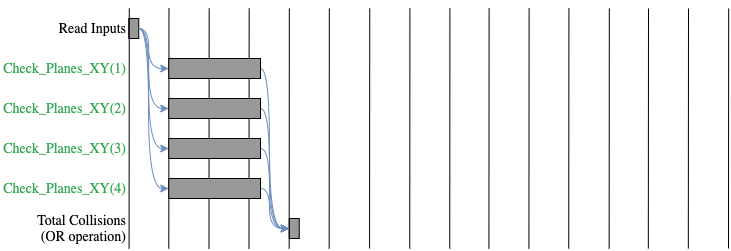
\includegraphics[width=\linewidth]{chapters/chapter3/img/timing4.png}
\caption{HoneyBee-C Timing Diagram. 4 instances of \texttt{Check\_Planes\_XY} module executing in parallel.}
\label{fig:hbb_timing_b}
\end{subfigure} \\

\end{tabular}
\mycaption{Timing Diagrams Showing Parallelization in HoneyBee-C}{. Again, these are generalizations for easy explanation of the concept of hardware parallelization. Full timing reports for each HoneyBee iteration can be found in Appendix \ref{section:honeybee_appendix_timing_reports}}
\label{fig:hbb_timing}
\end{centering}
\end{figure}

        Just focussing on the computation of the $xy$-oriented planes, Figure \ref{fig:hbc_timing} shows how \gls{HB-B} than having one instance of the module execute 4 times sequentially. \gls{HB-C} implements greater parallelism by instantiating 4 module instances to execute sequentially. \gls{HB-C}, as a result, exceeded the performance benchmark and was of an acceptable area, as shown in Table \ref{table:HBC_results} and Figure \ref{fig:benchmark_3}

        % @Author: AnthonyKenny98
% @Date:   2020-04-08 15:34:16
% @Last Modified by:   AnthonyKenny98
% @Last Modified time: 2020-04-08 19:39:39
\begin{table}[H]
\begin{center}
\begin{tabular}{|c|c|c|}
    \hline
    \textbf{Metric}             & \textbf{Specification} & \textbf{Synthesis Result} \\
    \hline
    Latency ($\mu$seconds/edge)  &   0.9  & \textcolor{mygreen}{0.53} \\
    \hline
    Throughput (edges/second)  &   1,111,111 & \textcolor{mygreen}{1,886,792} \\
    \hline
    FPGA Area \glspl{LUT} & 274,080  & \textcolor{mygreen}{185,663} \\
    \hline
\end{tabular}
\mycaption{Synthesis Results for HB-C with $\epsilon = 4$}{}
\label{table:HBC_results}
\end{center}
\end{table}

        % @Author: AnthonyKenny98
% @Date:   2020-04-08 17:54:49
% @Last Modified by:   AnthonyKenny98
% @Last Modified time: 2020-04-08 17:58:46
\begin{figure}[H]
\begin{centering}
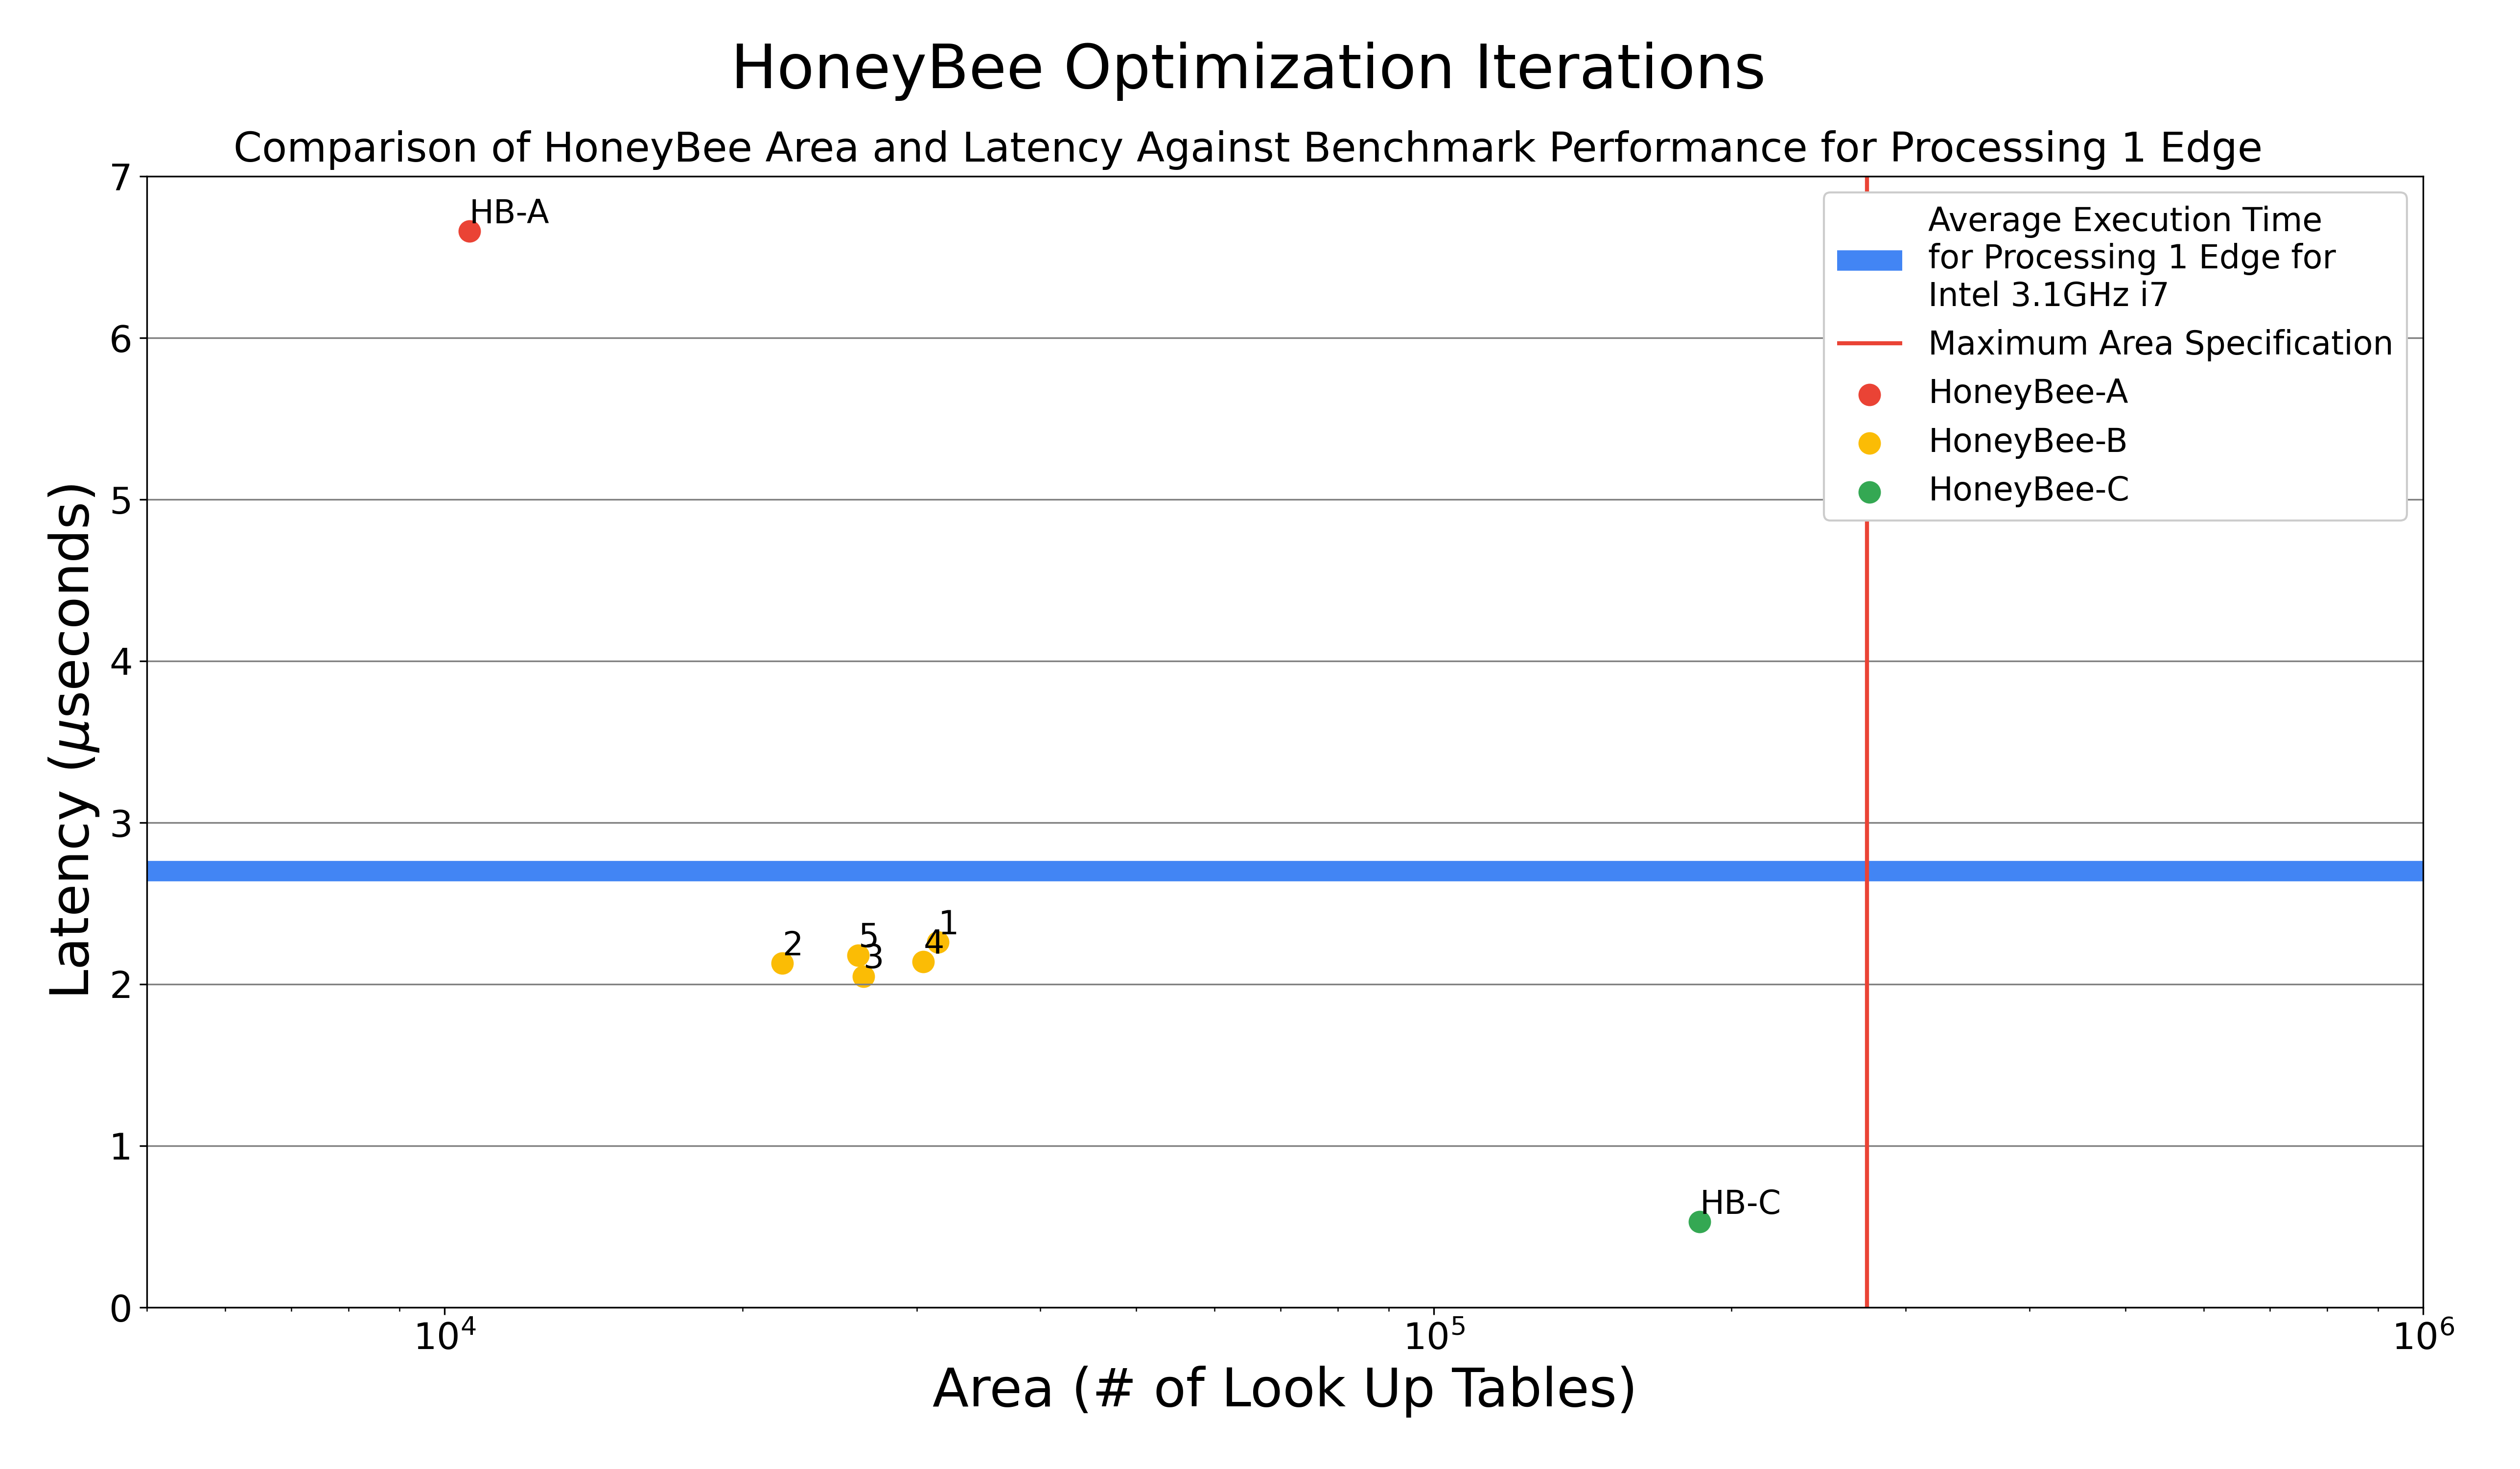
\includegraphics[width=\linewidth]{chapters/chapter3/img/benchmark_3.png}
\mycaption{}{}
\label{fig:benchmark_3}
\end{centering}
\end{figure}

% Chapter 4
\chapter{Motion Planning Architecture}
    \label{chap:MotionPlaningArchitecture}
    % @Author: AnthonyKenny98
% @Date:   2020-02-26 09:00:23
% @Last Modified by:   AnthonyKenny98
% @Last Modified time: 2020-02-26 09:04:23

\section{RISC-V ISA}

\section{Extending RISC-V}

\section{PhilosophyV}

% Conclusion
\chapter{Conclusion}
    % @Author: AnthonyKenny98
% @Date:   2020-04-10 23:01:04
% @Last Modified by:   AnthonyKenny98
% @Last Modified time: 2020-04-11 02:39:34

\section{Summary of Results}
    \subsubsection{Motion Planning in Software}
        The Rapidly-exploring Random Tree algorithm was successfully implemented in C. \\Rigourous experimentation was conducted to determine the optimal set of parameter values for quickly finding a collision-free path with high probability for a given map size. Once these optimal parameters were determined for different map sizes, thousands of simulations were run to find the bottleneck function of \gls{RRT}. It was found that the edge collision detection function consumed as much as 70\% of CPU execution time in \gls{3D}.

    \subsubsection{Motion Planning in Hardware}
        The HoneyBee unit was designed to implement the computation of edge intersections. High levels of hardware parallelization were utilized to reduce the latency of computing one edge from 6.66 $\mu$seconds to 0.53 $\mu$seconds. This translated to an improved throughput of 1,886,792 edges/second from (150,150 edges/second). Moreover, this was achieved in an acceptable area-on-FPGA.

    \subsubsection{Motion Planning Architecture}
        The Xedgcol non-standard RISC-V extension was defined. This ISA extension introduces two new instructions (\texttt{ECOL} and \texttt{LI.e}), along 6 new floating-point registers \texttt{e0-e5}. This extension reduces the number of instructions required to compute collisions for one edge from tens of thousands to only one (if you include the 6 LI.e calls to load the coordinate, then it requires seven). Philosophy V, a RISC-V processor, was implemented from the ground up to verify the extension. HoneyBee was implemented into PhilosophyV and tests of the Xedgcol extension conducted. The extension performed as defined.

    \begin{table}[H]
    \begin{center}
    \begin{tabular}{|c|c|}
    
    \end{tabular}
    \end{center}
    \end{table}

\section{Evaluation of Success}
    This thesis had four objectives:

    \begin{center}
    \bigskip\noindent\fbox{
    \parbox{0.9\textwidth}{
        \begin{center}        
        \textbf{Project Objectives} \\
        \end{center}
        \begin{enumerate}
            \item Determine the computational bottleneck of a commonly used motion planning algorithm.
            \item Implement a functional hardware module to replace the bottleneck function.
            \item Define a motion planning extension to the RISC-V ISA 
            \item Build a fully functional motion-planning processor that implements the extended RISC-V ISA
        \end{enumerate}
    }} \\
    \end{center}

    The first objective was achieved. \gls{RRT} was implemented from scratch, which may cast doubt as to how accurately its performance reflects real world implementations. The edge collision function was in fact implemented very realistically. The \gls{UAV} was represented as a 3D rectangular prisim and edge collision detection was based on solid geometric principles. \\
    If anything, more time was spent making sure that the edge collision function was as fast as possible in software, rather than on the other 4 key functions. The function that finds the nearest node in the graph was the second most computationally intense. There are many proven algorithmic optimizations for this function that were not applied in this implementation. Therefore, any uncertainty in the results of \gls{RRT} analysis would in fact \textit{under-represent} the computational load of edge collision detection. \\

    The second objective was also succesfuly completed. HoneyBee acheived a reduction in latency that was greater than its specification. HB-C could compute edge collisions 5 times faster than a professionally developed multi-core processor from Intel. Admittedly, once this performance was achieved, no further development was attempted. There still exists the opportunity for slight area optimizations and potentially even greater reductions in latency, though they would most likely be marginal. \\

    Of most significance to the overall goal of this thesis is the third objective. Successfully defining a RISC-V extension is the most compelling evidence for the future application of RISC-V in developing motion planning specific processors. \\
    The Xedgcol extension is simple and effective. This thesis took the approach of defining an instruction that would execute an entire function of RRT (edge collision). Since edge collision detection is required in most motion planning algorithms, the Xedgcol extension is widely applicable in the space. Another benefit of the Xedgcol design is how easy it is to implement in microarchitecture. The instructions were formatted in a way that reduced the the extra logic required for instruction decoding. Furthermore, designing a hardware unit like HoneyBee, while somewhat challenging, is made quite easy with tools such as \gls{HLS}. \\
    To cite some disadvantages of its design, it is perhaps not very elegant. It condenses an entire function into one instruction, which, while simple, does not afford an assembly programmer much flexibility. It also ``overarchitects'' for a certain implementation. There isn't really any other way to implement this particular extension other than implementing a hardware unit similar to HoneyBee (this does show, however, just how specific custom extensions can be).\\
    That being said, it does serve its purpose. It follows RISC-V convention and it correctly, simply, and effectively defines instruction set architecture for motion planning purposes.

    The fourth objective was to  desiging a RISC-V motion plannning processor. It was alluded to in Chapter 4 that this was not a fast processor. This is true; however, it was designed with simplicity in mind, for the purpose of verification, not performance. It correctly implements the RV32I\_Xedgcol instruction set, and verifies that the Xedgcol extension is compatible with the RV32I base intruction set. For the scope of this thesis, this was a success.

\section{Future Work}
    The overall mission of this thesis was:

    \begin{center}
    \bigskip\noindent\fbox{
        \parbox{0.8\textwidth}{
        \begin{center}
            \textbf{Mission} \\
            To present a proof-of-concept for extending and implementing RISC-V to develop motion planning specific processors.
        \end{center}
        }
    } \\
    \end{center}
    The driving motivation for this mission is that RISC-V has not yet been embraced by computer architects looking to improve computation of motion planning. Autonomous robots, and in particular, autonomous \glspl{UAV}, have the potential to change the world in which we live. Imagine warehouses filled with swarms of autonomous \glspl{UAV}, picking and packing orders without a human in sight. Imagine operations being carried out in dangerous, complex environments by drones with full autonomy. For this to be realised, however, motion planning specific processors need to be developed. Whereas commercial \glspl{ISA} present many barriers for doing this; RISC-V is all but designed for it. Suprisingly though, at the time of writing, there has been no published work on the application of RISC-V for developing motion planning specific processors. It is hoped that this thesis may encourage efforts to be made in this space, perhaps in one of the following areas.

    \subsubsection{Edge Collision Hardware}
    As mentioned above, the optimization of HoneyBee stopped once performance specifications for this project were met. It is feasible that there is a non-trivial amount of latency reduction still available with further optimization. Alternatively, perhaps there are other approaches to accelerating edge collision in hardware. Even if not within the RISC-V ecosystem, achieving faster motion planning will at some level depend on reducing the computational load of edge collision detection.

    \subsubsection{Production Quality RV32I\_Xedgcol Processor}
    It was well beyond the scope of this thesis to implement a production quality processor. It would be an interesting experiment to run comparison tests of RRT execution time between a general purpose Intel CPU and a professionally developed, multi-core RISC-V processor that implements the Xedgcol extension.

    \subsubsection{Better Motion Planning Extensions}
    The Xedgcol extension has some drawbacks that were highlighted above. As a proof of concept, it was very successful, but the biggest opportunity for future work lies in the development of better motion planning extensions. As more computer architects work on these extensions and better extensions are defined, the more of a developer following they get. This developer community builds, shares, and improves the extension and the toolchains for implementing that extension. For example, there is no compiler support for the Xedgcol extension - using it has to be done manually in assembly code, rather than high level languages. Compiler support may be implemented for a very popular non-standard extension. Of all potential future work to come from this thesis, it is hoped that the active development of RISC-V motion planning extensions occurs.

    \bigskip


    \noindent To conclude with a call to arms: This thesis provides a proof-of-concept for developing application specific processors for RISC-V with relative ease. Instruction Set Architecture is the most important interface of a computer, and RISC-V is the first commerically viable opportunity to open up this interface to the wider developer community. It is not an opporunity to be neglected. If this humble prototype can be a convincing argument for this, then it will be considered a success by its author. 


\begin{appendices}

\chapter{Project Repository}
\lhead{Appendix \thechapter} 
    \label{appendix:repository}
    % @Author: AnthonyKenny98
% @Date:   2020-02-23 14:22:13
% @Last Modified by:   AnthonyKenny98
% @Last Modified time: 2020-02-23 14:23:03

\todo[inline]{TODO: Provide information about this project's repository}

\chapter{RRT Supporting Documentation}
    \label{appendix:rrt_appendix}
    % @Author: AnthonyKenny98
% @Date:   2020-03-19 12:56:13
% @Last Modified by:   AnthonyKenny98
% @Last Modified time: 2020-04-10 14:55:54

\section{Justification of Modelling UAV as Prism}
\label{section:rrt_appendix_modelling}
    While it is possible for a \gls{UAV} to be modelled in precise detail, taking into account its exact shape, more often \glspl{UAV} are modelled as a 3D prism in motion planning problems, for the following reasons:
    \begin{itemize}
    \item It is a rare case that the negative space gained by modelling in such detail is utilised
    \item Representation of the drone's configuration is much more complex.
    \item Computing edge collisions is much more computationally intensive.
    \end{itemize}

    % @Author: AnthonyKenny98
% @Date:   2020-04-05 12:55:29
% @Last Modified by:   AnthonyKenny98
% @Last Modified time: 2020-04-05 15:43:13

\begin{figure}[H]
\begin{centering}

\begin{tabular}{cc}
\begin{subfigure}{0.45\linewidth}
    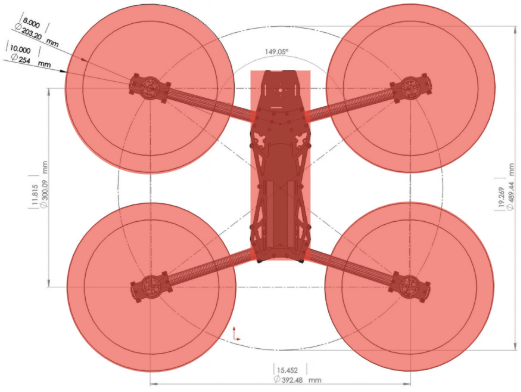
\includegraphics[width=\linewidth]{appendices/rrt/img/DroneNegSpace.png}
    \caption{}
    \label{subfig:dronenegspace}
\end{subfigure}
\begin{subfigure}{0.45\linewidth}
    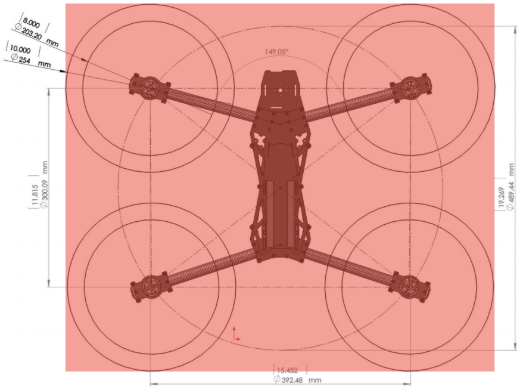
\includegraphics[width=\linewidth]{appendices/rrt/img/DroneRecPrism.png}
    \caption{}
    \label{subfig:dronerecprism}
\end{subfigure}
\end{tabular}
\caption[Modelling a UAV as a Rectangular Prism]{Modelling a \gls{UAV} as a Rectangular Prism. Red highlight demonstrates the model, overlayed over the exact schematic. Figure \ref{subfig:dronenegspace} shows how a drone can be modelled in high detail, but gains little useful free space when compared with Figure \ref{subfig:dronerecprism}, which models a drone as a rectangular prism.\cite{Thingbits}}
\label{fig:dronemodelling}
\end{centering}
\end{figure}

\section{Full Technical Specifications for RRT Implementation}
\label{section:rrt_appendix_tech_specs}
    % @Author: AnthonyKenny98
% @Date:   2020-04-05 14:09:51
% @Last Modified by:   AnthonyKenny98
% @Last Modified time: 2020-04-05 16:18:12

\begin{table}[H]
\begin{center}
\begin{tabular}{|p{.2\linewidth}|p{.74\linewidth}|}
    \hline
    \multicolumn{2}{|c|}{\textbf{General Specifications}} \\
    \hline
    \textbf{Requirement}             & \textbf{Description and Justification} \\
    \hline
    Implemented in C/C++    & 
        As outlined in Section \ref{subsection:project_structure}, the critical step in determining the design of specialized hardware to accelerate \gls{RRT} is CPU performance analysis of the algorithm to determine computational hot-spots. Implementations in C allow for the use of certain CPU profiling tools, described in Section \ref{subsubsection:vtune}, unlike higher-level languages such as Python. \\
    \hline
    3D Workspace            & 
        The computational requirements of \gls{RRT} in \gls{3D} differs somewhat to that in \gls{2D}. Since autonomous \glspl{UAV} operate in 3D space, it was neccesary to have a \gls{3D} implementation to analyse. \\
    \hline
    \Gls{UAV} modelled in \gls{3D} as a rectangular prism  & 
        In theory, it is possible to model a \gls{UAV} much more precisely than a rectangular prism, taking into account its shape and negative space. However, in reality, modelling a \gls{UAV} as a \gls{3D} rectangular prism, defined by coordinates $\{x, y, z\}$ and Euler angles $\{\alpha, \beta, \gamma \}$, is more than sufficient (and more efficient). See Appendix \ref{section:rrt_appendix_modelling} for justification of this. \\
    \hline
    Mathematically Complete Collision Detection & 
        When \gls{RRT} is implemented for educational purposes, the edge collision calulations are often simplified to a sampling model which is \gls{probabilistically complete} but not \gls{mathematically complete}. In other words, it will catch most collisions by sampling a number of points along each edge, but there is always a possibility of an undetected collision. In real world applications, collisions must be calculated by method of geometric intersection to ensure all collisions are detected. \\
    \hline
\end{tabular}
\caption{General Technical Specifications for \gls{RRT} Implementation}
\label{table:RRT_Tech_Specs_General}
\end{center}
\end{table}

\begin{table}[H]
\begin{center}
\begin{tabular}{|p{.2\linewidth}|p{.74\linewidth}|}
    \hline
    \multicolumn{2}{|c|}{\textbf{Required Parameters}} \\
    \hline
    \textbf{Parameter}   & \textbf{Description and Justification} \\
    \hline
    $\epsilon$ (a.k.a. $\Delta q$) & 
        The maximum difference between two configurations. Larger values of $\epsilon$ can solve less obstacle dense problems faster, but take longer to solve problems with tight corners.\\
    \hline
    $K$ &
        The maximum number of configurations. This is largely correlative to the amount of time the user will allow the algorithm to run. Larger values of $K$ will take longer but generate better paths, while smaller values will execute for less time but generate more jagged paths or may not reach the goal node. The value of $K$ was varied to find the minimum execution time while still reaching the goal with high probability. \\
    \hline
    $DIM$ &
        The upper bound of each axis of a $DIM\times DIM\times DIM$ Workspace. Larger values leave more space to be explored, and thus require larger values of $K$ to reach the goal with high likihood. \\
    \hline
    Goal Bias &
        The given probability that the graph will extend the graph $\epsilon$ distance from an existing configuration to a new configuration in the direction of the goal. \\
    \hline
\end{tabular}
\caption{Requiremed Parameters for \gls{RRT} Implementation}
\label{table:RRT_Tech_Specs_Parameters}
\end{center}
\end{table}

\section{Assessment of Existing RRT Implementations}
\label{section:rrt_appendix_existing_implementations}
    % @Author: AnthonyKenny98
% @Date:   2020-04-05 13:32:41
% @Last Modified by:   AnthonyKenny98
% @Last Modified time: 2020-04-05 13:46:28

\begin{table}[H]
\begin{centering}
\begin{tabular}{|p{0.2\linewidth}|p{0.15\linewidth}|p{0.15\linewidth}|p{0.15\linewidth}|p{0.15\linewidth}|}
\hline
Repository  & Language  &  Workspace Dimension  & Object Model & Algorithmic Correctness \\
\hline
RoboJackets\cite{RoboJackets2019}   & \textcolor{mygreen}{C++}    &       &       & \\
\hline
\end{tabular}
\caption[Evaluation of Existing Open-Source Implementations of RRT]{Evaluation of Existing Open-Source Implementations of RRT. Links to Github repositories can be found in the Bibliography.}
\end{centering}
\end{table}

\section{Implementation of Key RRT Functions}
\label{section:rrt_appendix_function_impl}
    % @Author: AnthonyKenny98
% @Date:   2020-04-05 21:30:06
% @Last Modified by:   AnthonyKenny98
% @Last Modified time: 2020-04-06 16:48:45

\bigskip
\begin{algorithm}[H]
    \caption{\texttt{getRandomConfig()} as implemented for \gls{RRT}}
    \SetAlgoLined
    \SetArgSty{textnormal}
    \begin{tabular}{l l}
    \textbf{Inputs:}    & Dimensionality $N$,\\ 
                        & Upper Axis Bound $DIM$ \\
    \textbf{Output:}    & Random Configuration $q$ \\
    \end{tabular}

        $q.x \leftarrow$ randomFloat($DIM$) \\
        $q.y \leftarrow$ randomFloat($DIM$) \\
        $q.\alpha \leftarrow$ randomFloat($2\pi$) \\
        \If{$N == 3$}{
            $q.z \leftarrow$ randomFloat($DIM$) \\
            $q.\beta \leftarrow$ randomFloat($2\pi$) \\
            $q.\gamma \leftarrow$ randomFloat($2\pi$) \\
        }
        \Return $q$;\\
\end{algorithm}
\bigskip
Where \texttt{randomFloat(max)} returns a float between 0 and \texttt{max}.

\bigskip
\begin{algorithm}[H]
    \caption{\texttt{findNearestConfig()} as implemented for \gls{RRT}}
    \SetAlgoLined
    \SetArgSty{textnormal}
    \begin{tabular}{l l}
    \textbf{Inputs:}    & Graph $G$, \\
                        & New Configuration $q_{new}$ \\
    \textbf{Output:}    & Nearest Configuration $q_{nearest}$ \\
    \end{tabular}

        $q_{nearest} \leftarrow$ $G$.$q_{init}$ \\
        \For{$k = 0$ to $G$.existing\_nodes}{
            \If{distance($q_{new}$, $G.q$[$k$]) < distance($q_{new}$, $q_{nearest}$)}{
                $q_{nearest} \leftarrow$ $G.q$[$k$] \\
            }
        }
        \Return $q_{nearest}$ \\
\end{algorithm}
\bigskip
Where \texttt{distance($q_1$, $q_2$)} returns the Euclidean distance between two configurations.

\bigskip
\begin{algorithm}[H]
    \caption{\texttt{stepFromNearest()} as implemented for \gls{RRT}}
    \SetAlgoLined
    \SetArgSty{textnormal}
    \begin{tabular}{l l}
    \textbf{Inputs:}    & Configuration in Graph $q_{nearest}$,\\ 
                        & New Configuration $q_{new}$, \\
                        & Goal Bias $B$, \\
                        & Maximum Step Distance $\epsilon$, \\
                        & Graph $G$ \\
    \textbf{Output:}    & Updated New Configuration $q_{new}$ \\
    \end{tabular}

        \If{distance($q_{nearest}$, $q_{new}$) > $\epsilon$}{
            \If{randomFloat($1$) < $B$}{
                $q_{new} \leftarrow $ stepTowardConfig($q_{nearest}$, $G$.$q_{goal}$) \\
            } \Else{
                $q_{new} \leftarrow $ stepTowardConfig($q_{nearest}$, $q_{new}$) \\
            }
        }
        \Return $q_{new}$;\\
\end{algorithm}
\bigskip
Where \texttt{stepTowardConfig($q_1$, $q_2$)} returns a configuration $\epsilon$ from $q_1$ in the direction of $q_2$.

\bigskip
\begin{algorithm}
    \caption{\texttt{configCollision()} as implemented for \gls{RRT}}
    \SetAlgoLined
    \SetArgSty{textnormal}
    \begin{tabular}{l l}
    \textbf{Inputs:}    & Dimensionality $N$,\\ 
                        & Occupancy Grid Map ($N$-Dimensional Array) $O$,\\ 
                        & Configuration $q$ \\
    \textbf{Output:}    & Boolean \\
    \end{tabular}

        \If{$N$ == 2 }{
            \Return $O$[gridLookup($q.x$)][gridLookup($q.y$)]
        }
        \Else{
            \Return $O$[gridLookup($q.x$)][gridLookup($q.y$)][gridLookup($q.z$)]
        }
\end{algorithm}
\bigskip
Where $O$ is a $N$-Dimensional array of booleans, with True representing an occupied grid and false representing an unoccupied one. \texttt{gridLookup()} is a function that maps a floating point coordinate to the correct integer of the grid in which it resides. For a map resolution of one, this is as simple as rounding a float down to an integer. \\

\begin{algorithm}[ht!]
    \caption{\texttt{configCollision()} as implemented for \gls{RRT} for 3D}
    \SetAlgoLined
    \SetArgSty{textnormal}
    \begin{tabular}{l l}
    \textbf{Inputs:}    & Edge $e$,\\ 
                        & Occupancy Grid Map (3-Dimensional Array) $O$,\\ 
                        & Maximum Step Distance $\epsilon$ \\
    \textbf{Output:}    & Boolean \\
    \end{tabular}
    
        $q_{min} \leftarrow $ minConfig($e.q_1$, $e.q_2$) \\
        \For{($x=  q_{min}.x$ to $q_{min}.x + \epsilon$)}{
            $q_{intersection} \leftarrow$ = edgeIntersectsPlane($e$, $x$) \\
            \If{$O$[$q_{intersection}.x$][$q_{intersection}.y$][$q_{intersection}.z$]}{
                \Return true
            }
        }
        \For{($y=  q_{min}.y$ to $q_{min}.y + \epsilon$)}{
            $q_{intersection} \leftarrow$ = edgeIntersectsPlane($e$, $y$) \\
            \If{$O$[$q_{intersection}.x$][$q_{intersection}.y$][$q_{intersection}.z$]}{
                \Return true
            }
        }
        \For{($z=  q_{min}.z$ to $q_{min}.z + \epsilon$)}{
            $q_{intersection} \leftarrow$ = edgeIntersectsPlane($e$, $z$) \\
            \If{$O$[$q_{intersection}.x$][$q_{intersection}.y$][$q_{intersection}.z$]}{
                \Return true
            }
        }
        \Return false
\end{algorithm}

While seemingly complex, the above algorithm merely steps through the mathematical process of checking the relevant $x$, $y$, and $z$ planes for a point of intersection with the edge $e$. It then looks up the \gls{OGM} $O$ to see if the grid corresponding with the point of intersection is occupied. If so, then it reports a collision be returning false. The function \texttt{edgeIntersectsPlane} follows the geometrical process of detecting a segment-plane intersection outlined in Appendix \ref{section:rrt_appendix_line_plane_intersection}. $q_{min}$ is calculated to be the origin point of the grid closest to the origin. In other words, the algorithm does not check for intersections throughout the entire map, only the maximum number of grids that could possible be intersected by the edge $e$, given the location of the two points of the edge, $e.p_1$ and $e.p_2$, and the maximum edge length $\epsilon$. The algorithm for \texttt{edgeCollision} in \gls{2D} can be inferred from the above, instead checking segment-line intersections for $x$ and $y$ lines.

\newpage
\section{Geometrically Determining Segment-Plane Intersection}
\label{section:rrt_appendix_line_plane_intersection}
    % @Author: AnthonyKenny98
% @Date:   2020-04-06 09:45:02
% @Last Modified by:   AnthonyKenny98
% @Last Modified time: 2020-04-06 15:27:15
The method of edge collision detection in this project's implementation of \gls{RRT} relies on detecting segment-plane intersections. The planes are always set up to be parallel with either the $xy$ plane, the $xz$ plane, or the $yz$ plane. Figure \ref{fig:parallelPlanes} demonstrates this point.

\begin{figure}[H]
\begin{centering}
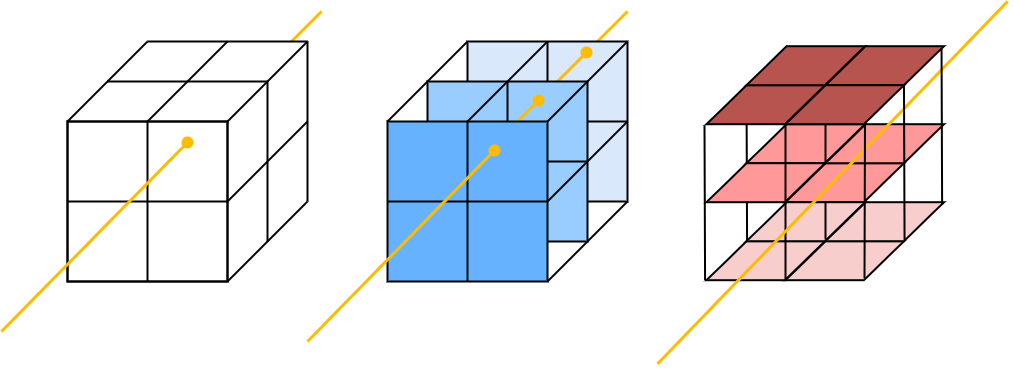
\includegraphics[width=\linewidth]{appendices/rrt/img/planes}
\caption{Using Parallel Planes to determine Edge Collisions with Grids}
\label{fig:parallelPlanes}
\end{centering}
\end{figure}

A plane can be defined by 3 points, $P_a$, $P_b$, and $P_c$. In practice, the points defining a plane parallel to the $xy$ plane would have the following points:

    $$P_a = (x,y,z)$$
    $$P_b = (x+\Delta x,y,z)$$
    $$P_c = (x,y+\Delta y,z)$$

Two vectors, $\vec{AB}$ and $\vec{AC}$ can be determined.

The normal to the plane is the cross product: 
    $$\vec{AB} \times \vec{AC}$$

And the equation of the plane written as:

    $$a(x-x_0) + b(y-y_0) + c(z-z_0) = 0$$
    $$ax + by + cz = ax_0 + by_0 + cz_0$$

Where $<a,b,c>$ is the normal to the plane and $(x_0, y_0, z_0)$ is one of the points $P_a$, $P_b$, or $P_c$.
The RHS can be set to equal $d$, leaving:

    $$ax + by + cz = d$$

Now, the equation of a line can be written in the form:

    $$ax + by + cz = 0$$

And can be parameterized in the following form:
    $$\begin{cases}
        x = & x_1 + t(x_2 - x_1) \\
        y = & y_1 + t(y_2 - y_1) \\
        z = & z_1 + t(z_2 - z_1) \\

    \end{cases}$$

To find the point of intersection, we substitute the equation of the line into the equation of the plane, yielding:

    $$a(x_1 + t(x_2 - x_1)) + b(x_1 + t(x_2 - x_1)) + c(x_1 + t(x_2 - x_1)) = d$$

Rearranging to find an expression for $t$:

    $$t = \frac{d - (ax_1 + by_1 + cz_1)}{a(x_2-x_1) + b(y_2-y_1) + c(z_2-z_1)}$$

Knowing $t$, we can find the point of intersection, $P_X$ to be:

    $$\begin{cases}
        x_X(t) = & x_1 + t(x_2 - x_1) \\
        y_X(t) = & y_1 + t(y_2 - y_1) \\
        z_X(t) = & z_1 + t(z_2 - z_1) \\
    \end{cases}$$

Finally, the following equalities are evaluated to see if the point lies on the segment:

    $$x_1 \leq x_X \leq x_2$$
    $$y_1 \leq y_X \leq y_2$$
    $$z_1 \leq z_X \leq z_2$$

If so, then the grids corresponding to the point of intersection can be marked as intersected.

\section{Timing Methodology of RRT Analysis}
\label{section:rrt_appendix_timing}
    % @Author: AnthonyKenny98
% @Date:   2020-04-06 08:00:17
% @Last Modified by:   AnthonyKenny98
% @Last Modified time: 2020-04-06 15:28:48

\subsubsection*{VTune Profiler}
    VTune Profiler is an application for software performance analysis. It provides functionality to examine hot-spots for CPU execution time through a top down analysis. The top down analysis tool shows the percentage of CPU time taken up by each function. It was used to initially profile the algorithm's performance.

    \subsubsection{Internal Timing}
        There are several limitations to using VTune Profiler. First, it can only profile software running on Intel processors, which implement the x86 \gls{ISA}. In anticipation of potentially needing to run performance analysis on a \gls{RISC-V} processor, another method was required. Secondly, VTune Profiler takes a long time to run, as it needs to conduct a lot of analysis that is extraneous to the purpose of this thesis. This became prohibitive when it came to conducting hundreds of tests for different parameterizations, with each test running \gls{RRT} a minimum of 100 times. Finally, it was not customizable to ignore certain parts of the implementation, such as logging functionality. While the implementation was designed in such a way that these should not intefere, it led to a lot of irrelevant data. A simple and effective alternative for measuring execution performance was to insert timing functionality into the software itself.

        Internal timing was implemented based on the inbuilt C \texttt{clock()} function and \\ \texttt{CLOCKS\_PER\_CYCLE} macro, and wrapping each function of interest in a performance tracking struct. This can be seen in the project's \gls{RRT} sub-repository under \texttt{performance.h}.

    \subsubsection*{Comparison}
        Before proceeding to use the internal timing method, it was important to verify that this method yielded similar results to VTune Profiler for the same program. Table \ref{table:timing_calibration} summarizes the results of analysis of a simple C executable. The program calls 5 functions, $\{A, B, C, D, E\}$, each a simple iteration in which a integer is incremented. Since the Internal Timing method returned similar results to the (trusted) VTune Profiler, it was considered to be a reliable method. While it was encouraging to see both methods returned similar results for absolute execution time, the more important metric was the similarity in percentage of total execution time. For good measure, a $\chi^2$ test of hypothesis was conducted and for one degree of freedom showed more that acceptable results.

        \begin{table}[H]
        \begin{center}
        \begin{tabular}{|m{0.09\linewidth}|m{0.16\linewidth}|m{0.16\linewidth}|m{0.16\linewidth}|m{0.16\linewidth}|m{0.09\linewidth}|}
        \hline
        \multirow{2}{*}{function} & \multicolumn{2}{c|}{Vtune Profiler} & \multicolumn{2}{c|}{Internal Timing}  & \multirow{2}{*}{$\chi^2$}\\
        \cline{2-5}
                    & time (s)  & time (\% total) & time (s) & time (\% total)  &   \\
        \hline
        A       & 0.488     & 57.4\%        & 0.497 & 57.6\%  &  0.00016       \\
        B       & 0.2       & 23.5\%        & 0.198 & 23.1\%  &  0.00002       \\
        C       & 0.102     & 12.0\%        & 0.099 & 11.5\%  &  0.00009       \\
        D       & 0.048     & 5.7\%         & 0.049 & 5.6\%   &  0.00002       \\
        E       & 0.012     & 1.4\%         & 0.019 & 2.2\%   &  0.00408       \\
        \hline
        \end{tabular}
        \end{center}
        \caption{Comparison of Timing Methods}
        \label{table:timing_calibration}
        \end{table}

\section{Execution Time of 2D and 3D RRT for Different Map Sizes}
\label{section:rrt_time_taken}
\begin{figure}[H]
\begin{centering}
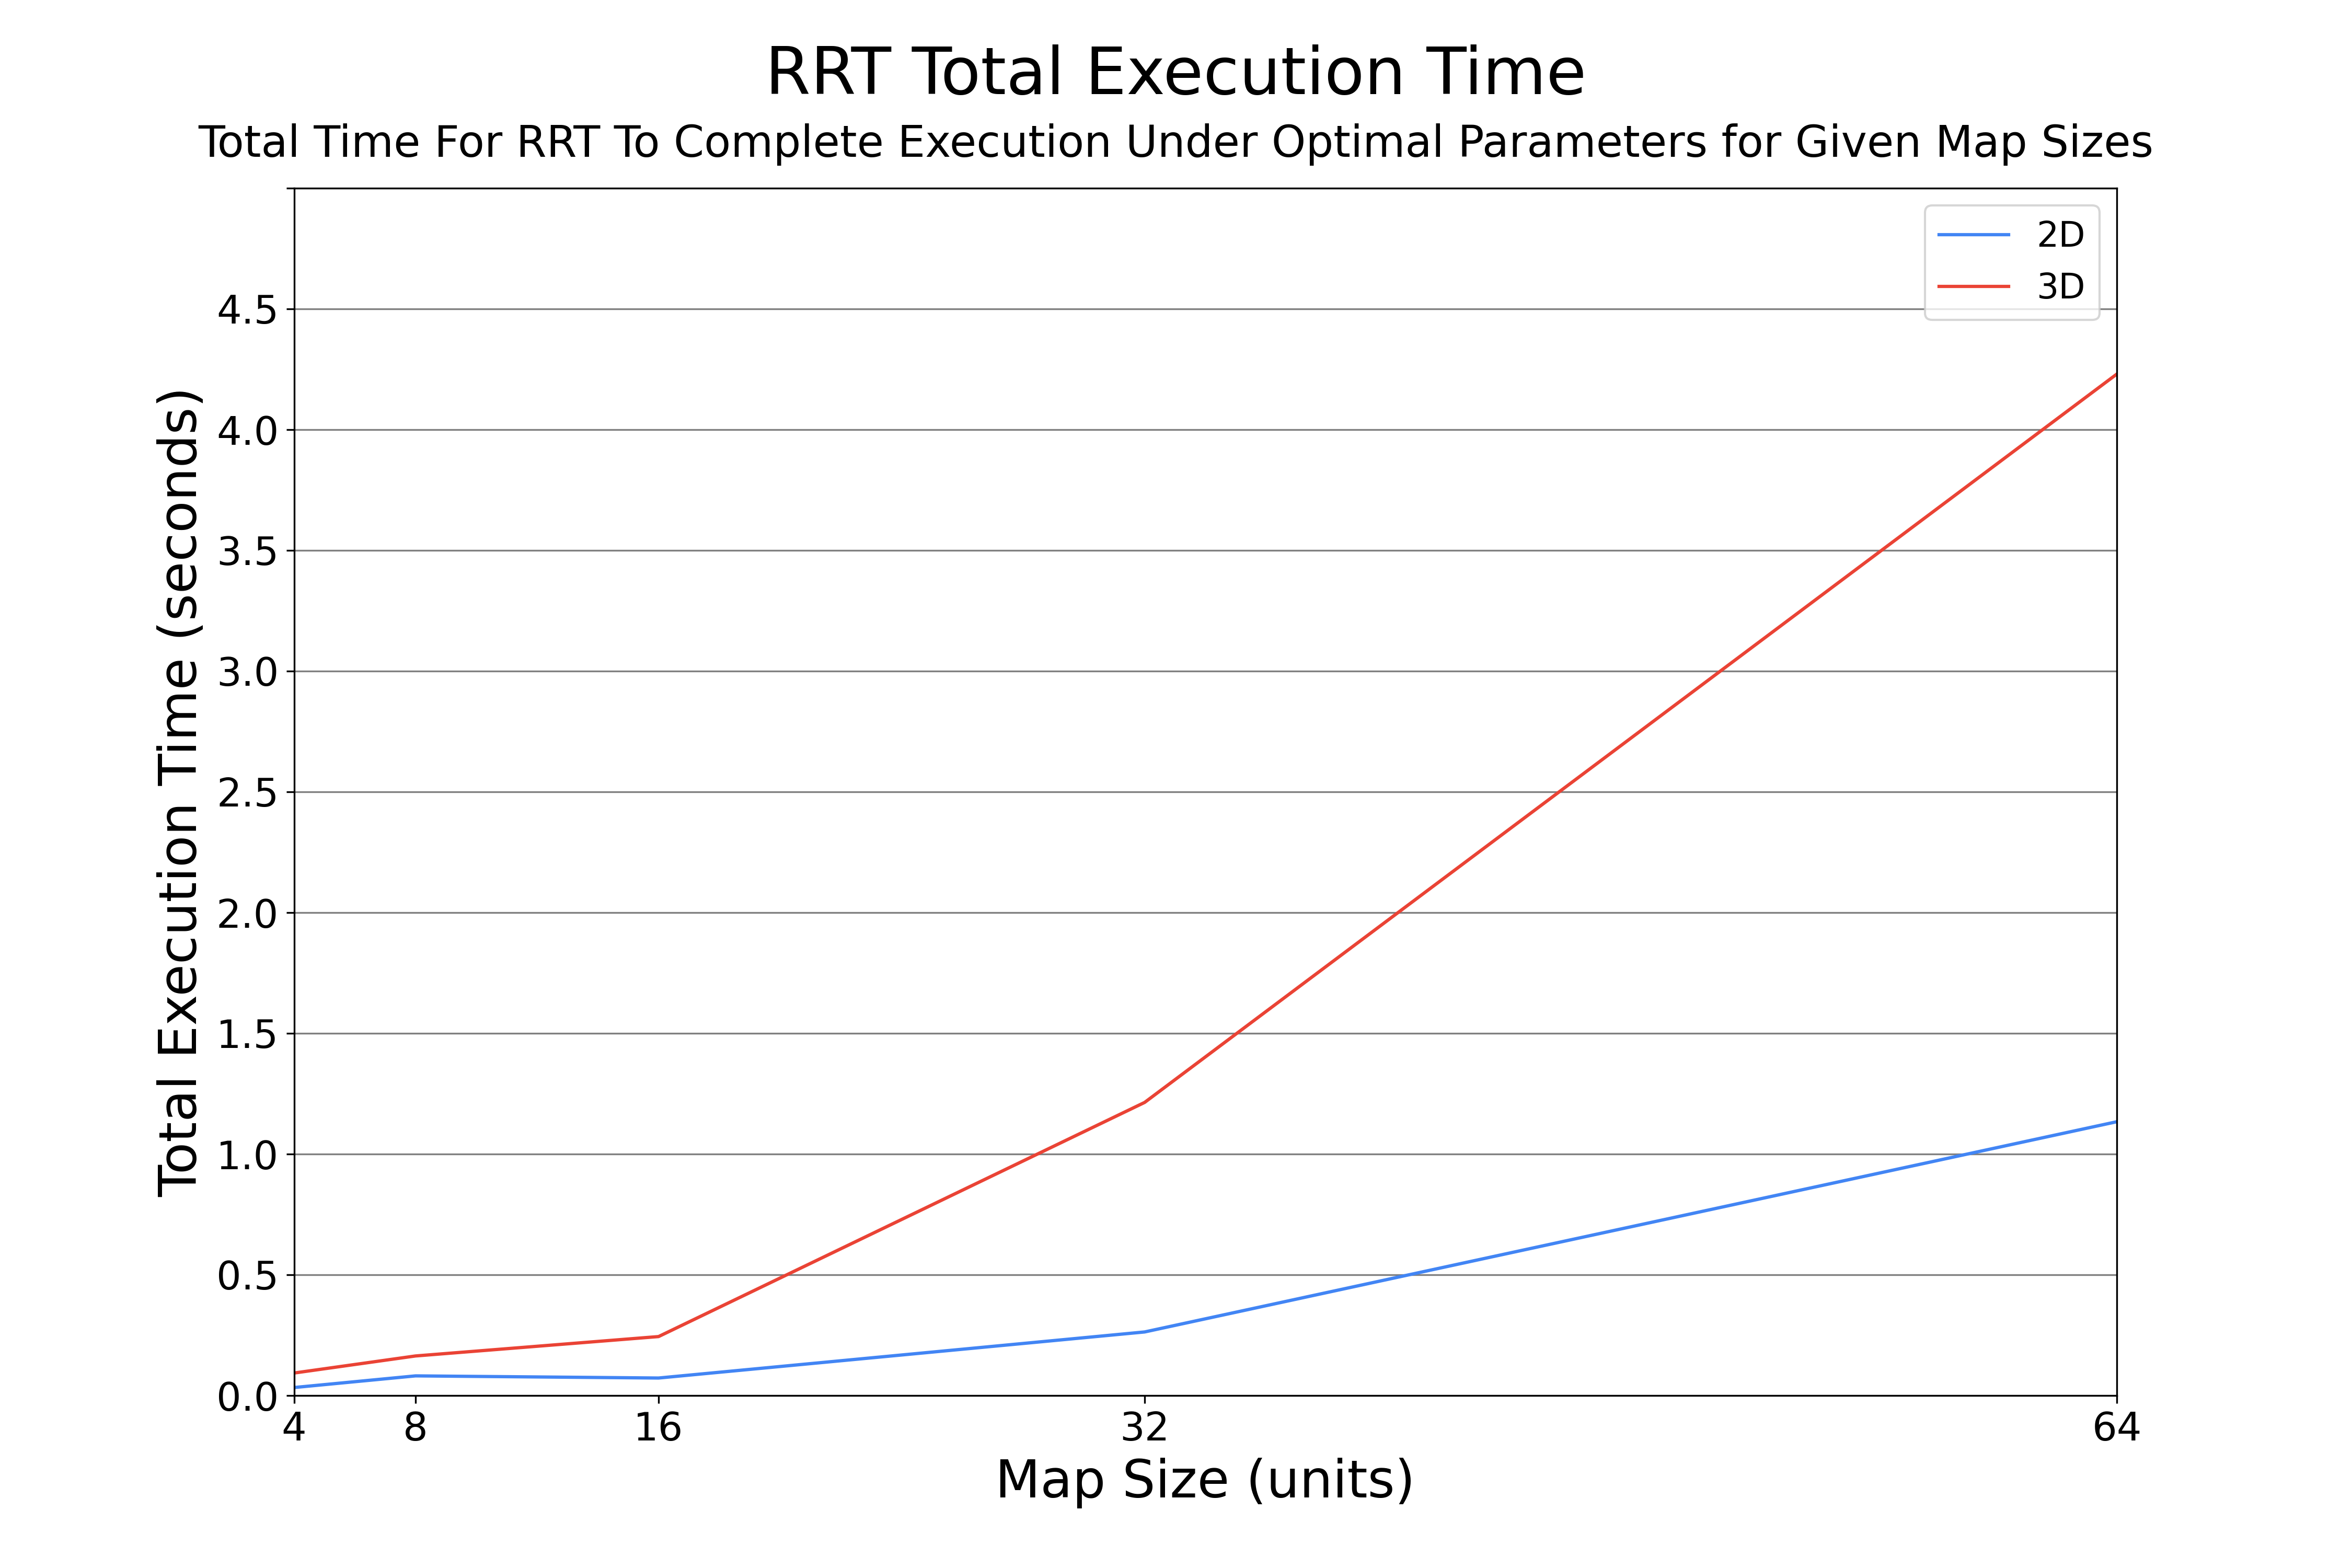
\includegraphics[width=0.65\linewidth]{chapters/chapter2/img/profiling/timing.png}
\caption[Increasing Total Execution Time of RRT with Map Size]{\textbf{Increasing Total Execution Time of RRT with Map Size}}
\label{fig:rrt_profiling_timing}
\end{centering}
\end{figure}


\chapter{HoneyBee Supporting Documentation}
    \label{appendix:honeybee_appendix}
    % @Author: AnthonyKenny98
% @Date:   2020-04-07 14:14:38
% @Last Modified by:   AnthonyKenny98
% @Last Modified time: 2020-04-08 19:09:49

\newpage
\section{Full Technical Specifications for Edge Collision Detection Unit}
    \documentclass[11pt, oneside]{article}      % use "amsart" instead of "article" for AMSLaTeX format
\usepackage{geometry}                       % See geometry.pdf to learn the layout options. There are lots.
\geometry{letterpaper}                          % ... or a4paper or a5paper or ... 
%\geometry{landscape}                       % Activate for rotated page geometry
%\usepackage[parfill]{parskip}          % Activate to begin paragraphs with an empty line rather than an indent
\usepackage{graphicx}               % Use pdf, png, jpg, or eps§ with pdflatex; use eps in DVI mode
                                % TeX will automatically convert eps --> pdf in pdflatex        
\usepackage{amssymb}
\usepackage{amsmath}
\usepackage{array}
\usepackage{float}
\usepackage{hyperref}
\hypersetup{
    colorlinks=true,
    citecolor=black,
    linkcolor=black,
    filecolor=magenta,      
    urlcolor=cyan,
}
\usepackage[printonlyused]{acronym}


\RequirePackage{../support/thesis}
\RequirePackage{../master/master}
% Import custom commands
\RequirePackage{../support/thesis}
\RequirePackage{../master/master}

%%%%%%%%%%%%%%%%%%%%%%%%%%%%%%%%%%%%%%%%%%%%%%%%%%%%%%%%%%

\title{\textsc{Technical Specifications} \\ 
	\small{for} \\ 
	\Large{\masterThesisTitle}}
\author{Anthony JW Kenny \\ \\
        Electrical Engineering \\
        Advisor: Vijay Janapa Reddi} 
\masterDateAndVersion 

\begin{document}
\maketitle


% ABSTRACT
% @Author: AnthonyKenny98
% @Date:   2019-10-30 22:35:34
% @Last Modified by:   AnthonyKenny98
% @Last Modified time: 2019-10-31 10:45:30

\abstract{This thesis aims to design RISC-V computer architecture that supports the fast execution of motion planning algorithms for drone applications. First, the computation of sampling-based motion planning algorithms commonly used in autonomous drones (such as \ac{RRT}, \ac{RRT*}, \ac{PRM}) will be profiled on an unmodified RISC-V processor. From this profiling, common bottlenecks and hotspots in execution will be identified. Based on these results, this project will extend the RISC-V \ac{ISA} and design a modified processor to support the extensions.}
% 78 words ^

% @Author: AnthonyKenny98
% @Date:   2019-10-30 22:48:26
% @Last Modified by:   AnthonyKenny98
% @Last Modified time: 2020-02-20 00:14:46

\section{Project Summary}

\subsection{Problem Statement}
Current processors cannot compute motion planning algorithms quickly enough for robots to operate in high complexity environments. Autonomous drones are a specific case of robots requiring real-time motion planning in complex environments. The state-of-the-art strategy of using a \ac{GPU} to accelerate the execution of these algorithms requires too much power to be cost-effective or feasible for drones to sustain flight for useful periods of time.
% 65 words ^

\subsection{End User}
The end user of this project is a developer of autonomous drones. Such developers have a need for computing hardware that executes motion planning algorithms faster and more power efficiently than existing methods. This thesis will provide a processor design that is synthesizable on an \ac{FPGA}, giving developers a processer for which a \ac{RTOS}, or bare metal code, can be written. 
Additionally, these developers have a requirement that using a new processor for a drone will not require a massive investment in re-development. As such, this thesis will provide the toolchain necessary to compile C code into executable instructions on the new processor.

\subsection{Project Goals} \label{subsection:projectGoals}
This thesis aims to design a RISC-V processor, optimized for motion planning computation, that is synthesizeable on an \ac{FPGA} and adheres to the requirements outlined in Section \ref{subsection:projectRequirements}. It will also provide the tools necessary to complile programs for the processor. 

The nature of research into accelerating computation through modified computer architecture is such that, when asked a question of how fast/efficient/small/etc a system must be, the answer is, with consideration to certain trade-offs, as fast/efficient/small/etc as it can be! Thus, when defining goals for certain metrics such as speed or power efficiency, this thesis will do so by comparing performance of the modified processor with benchmark performance of an unmodified, off-the-shelf RISC-V processor synthesized on the same \ac{FPGA}.

\subsection{Project Requirements} \label{subsection:projectRequirements}
Table ~\ref{table:projectRequirements} outlines conceptually the requirements of the project.

\begin{table}[H]
\begin{centering}
\begin{tabular}{| m{0.25\linewidth} | m{0.75\linewidth} |}
\hline
\textbf{Requirement}       & \textbf{Description} \\
\hline
RISC-V Compliance   & This project will extend the RISC-V \ac{ISA} to add new instructions. The contstraint of RISC-V compliance means that the new ISA must follow RISC-V conventions, and that the processor can implement any program compiled into the original RISC-V ISA.\\
\hline
Synthesizable       & The processor design must be such that it is practically useable by drone developers. Since having such a processor design produced on a chip is beyond this project's scope, this project must deliver a processor defined in an \ac{HDL} that is synthesizable on an FPGA.\\
\hline
Speed               & One of the motivating factors of this project is the need for motion planning algorithms to execute faster for autonomous drones to become more useful in real world applications. \\
\hline
Power consumption   & The second motivating factor is the need for computation aboard drones to be as power efficient as possible to enable them to remain in flight for long enough periods of time.\\
\hline
\end{tabular}
\caption{Conceptual Outline of Project Requirements}
\label{table:projectRequirements}
\end{centering}
\end{table}

\subsubsection{Stakeholder Map} 
\begin{figure}[H]
\begin{centering}
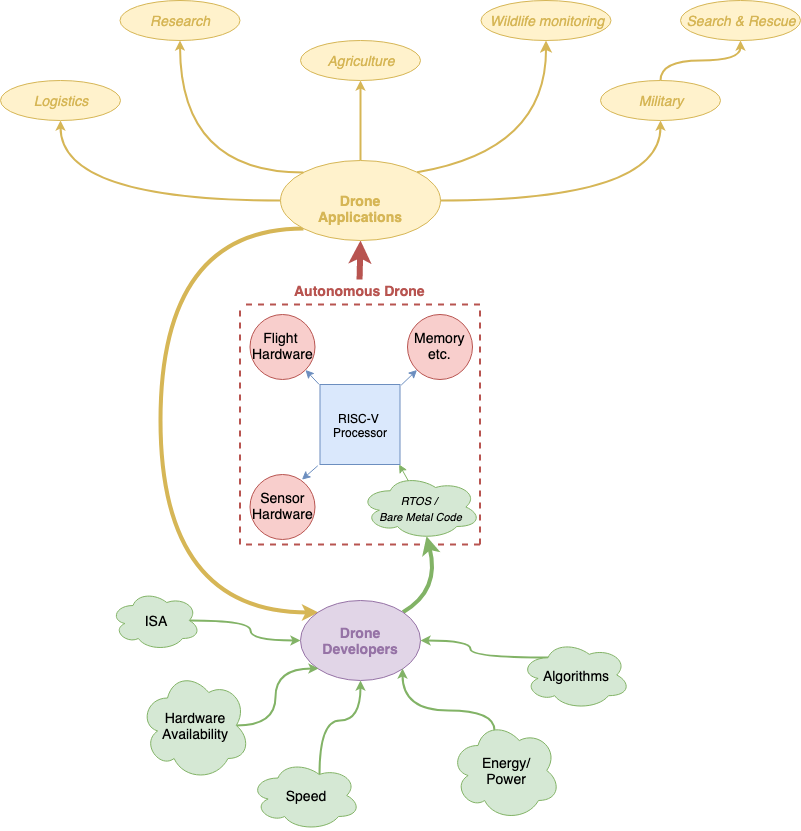
\includegraphics[width=\linewidth]{img/stakeholderMap.png}
\caption{Stakeholder Map}
\label{fig:stakeholderMap}
\end{centering}
\end{figure}

The processor that this thesis aims to design is highlighted in the center of the stakeholder map as the blue box, labelled "RISC-V Processor". It resides within the system of a generic Autonomous Drone, interfacing with flight, sensor, and memory hardware. On this processor, runs either a \ac{RTOS} or bare metal code, designed by the Drone Developer. A Drone Developer is influenced in their designs by the factors in green clouds, as well as from the requirements of Drone Applications.

\section{System Model Diagram}

\begin{figure}[!htbp]
\begin{centering}
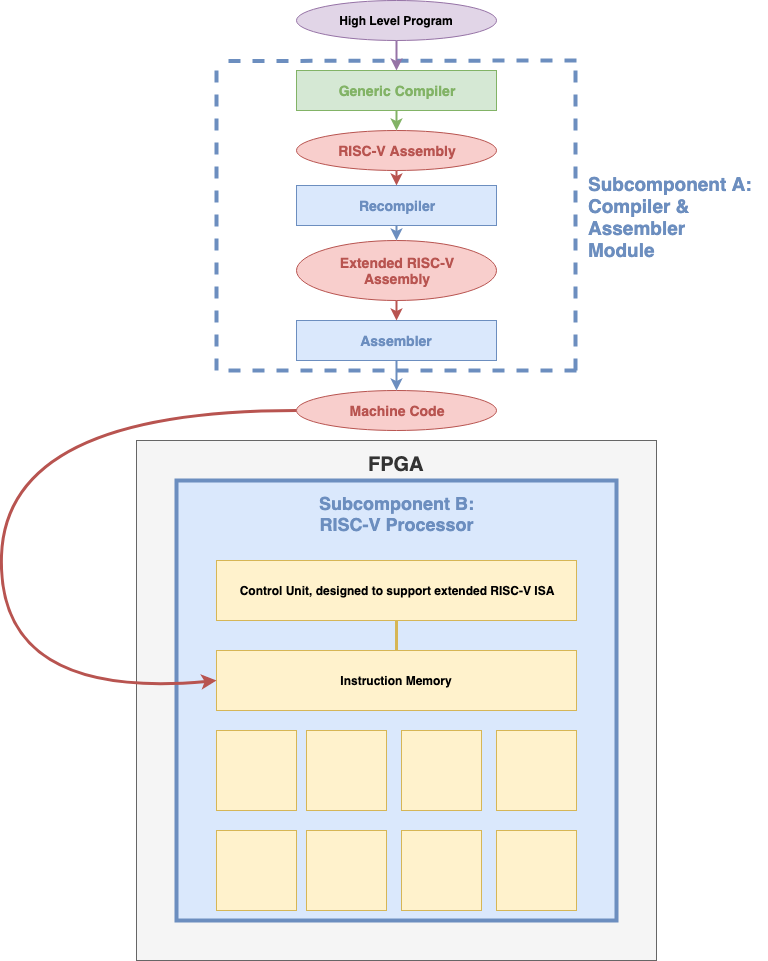
\includegraphics[width=\linewidth]{img/systemDiagram.png} 
\caption{System Diagram}
\label{fig:systemDiagram}
\end{centering}
\end{figure}

There are two subcomponents to this project's design, shown in Figure \ref{fig:systemDiagram}. First the Compiler \& Assembler Module, which takes Programs written by a drone developer in C as an input, and outputs machine code to be loaded into the instruction memory of the processor. The second subcomponent is the RISC-V Processor, with the basic representation above showing the control unit, the instruction memory, and other modules that will make up the processor. The exact design of the processor will depend on results of profiling and which extended instructions need to be supported. This design will be loaded onto an FPGA.

\clearpage
% @Author: AnthonyKenny98
% @Date:   2019-10-31 10:05:27
% @Last Modified by:   AnthonyKenny98
% @Last Modified time: 2019-10-31 10:47:45


\section{Overall System Specifications}
Let the overall system be defined as 2 part: the Processor Module and the Compiler/Assembler Module. \\
The following subsections detail the technical specifications of the overall system. System specifications based on comparison with benchmarks will be compared against the same programs running on an unmodified, off-the-shelf RISC-V processor synthesized on the same \ac{FPGA}.
\subsection{Speed}
\subsubsection{Quantitative Description}
This project must deliver a system that, given a program that implements, in C, an algorithm often used in autonomous drone motion planning, executes said algorithm an order of magnitude faster than a generic RISC-V processor.

\subsubsection{Justification}
This project aims to achieve a speedup of at least one order of magnitude (10 times) when compared to benchmark performance, in the execution of pure motion planning algorithm programs.
The justification for an order of magnitude speedup comes from similar projects that accelerated motion planning algorithms, acheiving speedups from between 1 and 3 orders of magnitude. These indclude approaches using external hardware accelerators\cite{Murraya}, reprogrammable hardware and parallelization on FPGAs\cite{Murray}\cite{Atay2006}\cite{Malik2015}, and chip redesigns\cite{Murrayb}\cite{Zhi}.

\subsubsection{Measurement}
There will be two broad stages of measurement for this metric. First, in simulation, the Vivado Design Suite\cite{Vivado} will allow the execution of a given compiled program to be timed on a simulated processor that is defined in an \ac{HDL}. Secondly, in synthesis, a to-be-determined tool will allow for me to time the execution of the same program, now on a processor physically synthesized on an FPGA. 

\subsection{Power Consumption}
\subsubsection{Quantitative Description}
This project must deliver a system that has comparable power consumption as an unmodified RISC-V processor operating on the same FPGA. Comparable will be defined as within a tolerance range of 10\%.
\subsubsection{Justification}
Power is defined as energy dissipated over time.\cite{AmericanElectricianHandbook} As such, when considering the application of this system in autonomous drones, we want to minimize the amount electrical energy committed to the computation of paths. Since the primary goal of this thesis is to reduce the execution time, it can aim to keep power use comparable between the benchmark system and the new system. If power remains roughly constant, but the time taken to execute a program is reduced 10 times, we should see a proportional improvement in energy efficiency.
\subsubsection{Measurement}
The Vivado Design Suite\cite{Vivado} will allow for simulated power consumption estimates, but the important measurement will be comparing the new processor to the unmodified processor on the FPGA, running the same program. I am still to determine how exactly to measure this, but the parameters for testing are known and shown above.


\section{Recompiler \& Assembler Specifications}
The first subcomponent of the system is the Compiler \& Assembler Module. It has two specifications, Correctness and Optimality. 
\subsection{Correctness}
\subsubsection{Quantitative Description}
This project must deliver a Compiler \& Assembler Module that, given a program defined in C, can compile and assemble this program into machine code, in a manner that follows the chosen ISA correctly. 
\subsubsection{Justification}
When announcing the IBM System/360 in 1964, IBM said the following: "Instruction Set Architecture is the structure of a computer that a machine language programmer must understand to write a correct program for that machine."\cite{IBM1964} That is, it is a contract between the compiler and the hardware, so that the compiler can write machine code that will work for a given computer processor. In this way, for a given ISA (whether RISC-V, or the extened RISC-V this project will design), the Compiler \& Assembler Module must adhere to that ISA to compile instruction sets that will execute correctly on the processor.
\subsubsection{Measurement}
Testing for correct compiling under the original RISC-V ISA is relatively simple. Does the Generic Compiler (which shouldn't be altered by this project) produce correct RISC-V Assembly. Then, the Recompiler module will operate on those RISC-V assembly instructions to produce a recompiled assembly instruction set that follows the project's extended RISC-V ISA. The Assembler will then assemble this into machine code that can be directly loaded into the processor's Instruction Memory. Testing for this required extensive and complete unit tests to be written during this project.

\subsection{Optimality}
\subsubsection{Quantitative Description}
This project must deliver a Compiler \& Assembler Module that, given certain extended instructions that this project defines, recompiles all regular RISC-V assembly code that is suitable for recompilation. 
\subsubsection{Justification}
The RISC-V \ac{ISA} is an ISA that supports user-level ISA extensions and specialized variants\cite{Isa2012}, which may allow the number of instructions per program to be reduced through clever redesign of a processor and new instructions. However, to reap the full performance rewards of these extensions, a compiler must use the new instructions whenever it is able.
\subsubsection{Measurement}
This will be challenging to measure. I plan to write extensive unit tests that will determine manually the optimal recomplication from RISC-V to extended RISC-V assembly, and then compare that to the output of the recompiler module. There will also be tests to check that these substitutions are occuring in larger, more complicated programs.

\section{Processor Specifications}
The second subcomponent of the system is the Processor Unit. It has two specifications, RISC-V Compliance and Syntheizability.

\subsection{RISC-V Compliance} \label{subsection:riscvCompliance}
\subsubsection{Quantitative Description}
The project must deliver a processor that is RISC-V Compliant, meaning that it can support any correctly compiled RISC-V Assembly Code.
\subsubsection{Justification}
A processor must be such that it supports the execution of all instructions defined in the \ac{ISA} for which it was designed. So too must this project's finished processor be able to correctly support any correctly compiled RISC-V assembly code. This may range from simple programs compiled into either the original or extended RISC-V \ac{ISA}, to complete operating systems, whether for drone applications or a generic linux distribution, for example. 
\subsubsection{Measurement}
The RISC-V organisation has provided a Github Repo for testing a processor for RISC-V compliance.\cite{Compliance} Once it passes this, this processor should be able to run any program or OS compiled into RISC-V assembly.

\subsection{Synthesizable}
\subsubsection{Quantitative Description}
The project must deliver a processor defined in an \ac{HDL} that is synthesizable on an FPGA for the project to be useful for drone developers. While this project will use and test with the Diligent Zync-7000 \ac{SoC}\cite{Zync}, the design should be synthesizable on most Zync boards.
\subsubsection{Justification}
Many papers that have worked in the area of accelerating motion planning algorithms for robot applications have delivered a finished product of a processor/accelerator design implemented in an \ac{HDL} for synthesis on an FPGA.\cite{Murray}\cite{Atay2006}\cite{Malik2015} This FPGA can then be used to control the robot or share computational load with a co-processor.
\subsubsection{Measurement}
Measurement for this specification is relatively simple. Once the processor is designed in an \ac{HDL}, it can be synthesized onto an FPGA using the Vivado Design Suite, given the design is synthesizable (although this is not always simple to achieve). If it is not synthesizable, the design suite will throw and error.
Finally, while the design should be correct and RISC-V compliant by the tests performed in section \ref{subsection:riscvCompliance}, to be safe, these compliance tests along with any other unit tests designed during this thesis will then be run on the \ac{FPGA} processor.
\clearpage

\section{List of Acronyms}
\input{\acronymsName}


\clearpage

\bibliography{\bibliographyName}
\bibliographystyle{ieeetr}


\end{document}  


\section{IEEE Standard for Floating-Point Arithmetic}
\label{section:honeybee_appendix_ieee}
    \todo[inline]{IEEE Standard for Floating-Point Arithmetic}

\section{Mapping HoneyBee's Output Sequence to a Grid-Map}
\label{section:honeybee_appendix_mapping}
    \todo[inline]{Mapping HoneyBee's Output Sequence to a Grid-Map}

\section{HoneyBee Handshake Control Protocol}
\label{section:honeybee_appendix_handshake}
    % @Author: AnthonyKenny98
% @Date:   2020-04-08 12:12:17
% @Last Modified by:   AnthonyKenny98
% @Last Modified time: 2020-04-08 12:26:20
\begin{table}[H]
\begin{centering}
\begin{tabular}{|p{0.2\linewidth}|p{0.7\linewidth}|}
\hline
\textbf{Port}   & \textbf{Description} \\
\hline
\texttt{start}  &
    This signal controls the block execution and must be asserted to logic 1 for the design to begin operation. It should be held at logic 1 until the associated output handshake \texttt{ready} is asserted. When \texttt{ready} goes high, the decision can be made on whether to keep \texttt{start} asserted and perform another transaction or set \texttt{start} to logic 0 and allow the design to halt at the end of the current transaction. If \texttt{start} is asserted low before \texttt{ready} is high, the design might not have read all input ports and might stall operation on the next input read. \\
\hline
\texttt{ready}  &
    This output signal indicates when the design is ready for new inputs. The \texttt{ready} signal is set to logic 1 when the design is ready to accept new inputs, indicating that all input reads for this transaction have been completed. If the design has no pipelined operations, new reads are not performed until the next transaction starts. This signal is used to make a decision on when to apply new values to the inputs ports and whether to start a new transaction should using the \texttt{start} input signal. If the \texttt{start} signal is not asserted high, this signal goes low when the design completes all operations in the current transaction. \\
\hline
\texttt{done}   &
    This signal indicates when the design has completed all operations in the current transaction. A logic 1 on this output indicates the design has completed all operations in this transaction. Because this is the end of the transaction, a logic 1 on this signal also indicates the data on the \texttt{return} port is valid. Not all functions have a function return argument and hence not all RTL designs have an \texttt{return} port. \\
\hline
\texttt{idle}   & 
    This signal indicates if the design is operating or idle (no operation). The idle state is indicated by logic 1 on this output port. This signal is asserted low once the design starts operating. This signal is asserted high when the design completes operation and no further operations are performed. \\
\hline
\end{tabular}
\mycaption{Description of the ports associated with the handshake protocol for HoneyBee}{. Adapted from Vivado HLS User Guide\cite{Xilinx2014}}
\end{centering}
\end{table}

\section{HoneyBee Interface Synthesis Report}
\label{section:honeybee_appendix_synthesis_report}
    % @Author: AnthonyKenny98
% @Date:   2020-04-08 15:51:15
% @Last Modified by:   AnthonyKenny98
% @Last Modified time: 2020-04-08 15:58:54
\begin{table}[H]
\begin{centering}
\begin{tabular}{|l|l|l|l|l|}
\hline
\textbf{RTL Ports}  & \textbf{Direction}    & \textbf{Bits} & \textbf{Protocol} & \textbf{C Type} \\
\hline
ap\_clk  & in & 1 & ap\_ctrl\_hs & return value \\
\hline
ap\_rst  & in & 1 & ap\_ctrl\_hs & return value \\
\hline
ap\_start  & in & 1 & ap\_ctrl\_hs & return value \\
\hline
ap\_done  & out & 1 & ap\_ctrl\_hs & return value \\
\hline
ap\_idle  & out & 1 & ap\_ctrl\_hs & return value \\
\hline
ap\_ready  & out & 1 & ap\_ctrl\_hs & return value \\
\hline
ap\_return  & out & 64 & ap\_ctrl\_hs & return value \\
\hline
edge\_p1\_x   & in & 32 & ap\_none & scalar \\
\hline
edge\_p1\_y   & in & 32 & ap\_none & scalar \\
\hline
edge\_p1\_z   & in & 32 & ap\_none & scalar \\
\hline
edge\_p2\_x   & in & 32 & ap\_none & scalar \\
\hline
edge\_p2\_y   & in & 32 & ap\_none & scalar \\
\hline
edge\_p2\_z   & in & 32 & ap\_none & scalar \\
\hline
\end{tabular}
\mycaption{HoneyBee Interface Synthesis Report}{ for $\epsilon = 4$. Results taken from Vivado HLS synthesis report.}
\end{centering}
\end{table}

\section{HoneyBee Timing Reports}
\label{section:honeybee_appendix_timing_reports}
    \todo[inline]{HoneyBee Timing Reports}

\section{HoneyBee-B Variants}
\label{section:honeybee_appendix_hbb_variants}
    \todo[inline]{HoneyBee-B Variants}

\chapter{Xedgcol Non-Standard Extension for Edge Collision Detection}
    \label{appendix:xedgcol_appendix}
    % @Author: AnthonyKenny98
% @Date:   2020-04-09 10:26:50
% @Last Modified by:   AnthonyKenny98
% @Last Modified time: 2020-04-11 01:47:38

This chapter describes version 1.0 of the Xedgcol Non-Standard ISA Extension for RISC-V.

The Xedgcol extension is designed to be implementable alongside any base ISA without reliance on any other extensions. For example, the Xedgcol instruction set requires support for floating point registers, which are not provided in the RV32I ISA. As such, it defines 6 new registers specifically for use with this ISA.

Xedgcol is a \textit{highly} specialized ISA extension, designed explicitly for accelerating motion planning.
Specifically, it is designed for the invocation of logic to compute the intersections of an edge with a grid space. The maximum length of the edge is 4 times the length of a single grid. This is relevant as a $4x4x4$ gridspace can be saved to two 32-bit x-registers.

\section{Xedgcol Register State}
The Xedgcol extension defines 6 new 32-bit floating-point registers, \texttt{e0-e5}. The term XELEN is used to desrive the width of these floating-point registers in the RISC-V ISA, and XELEN=32 for this extension.
Table \ref{table:Xedgcol_registers} shows the additional register state defined by Xedgcol. 
\begin{table}[H]
\begin{center}
\begin{tabular}{|c|c|c|}
\hline
\textbf{Register} & \textbf{ABI Name} & \textbf{Description} \\
\hline
\texttt{e0}     & \texttt{px0}      & X coordinate of edge's first point \\
\hline
\texttt{e1}     & \texttt{py0}      & Y coordinate of edge's first point \\
\hline
\texttt{e2}     & \texttt{pz0}      & Z coordinate of edge's first point \\
\hline
\texttt{e3}     & \texttt{px1}      & X coordinate of edge's second point \\
\hline
\texttt{e4}     & \texttt{py1}      & Y coordinate of edge's second point \\
\hline
\texttt{e5}     & \texttt{pz1}      & Z coordinate of edge's second point \\
\hline
\end{tabular}
\mycaption{Xedgcol Register State}{}
\label{table:Xedgcol_registers}
\end{center}
\end{table}

\section{Referencing Xedgcol Registers}
Since only 6 registers are defined and they are only referenced by the instructions defined in this ISA, it is possible for them to be referenced using only 3-bit values. This allows for more bits in the instructions to be used for immediate values.

\section{Load Immediate Edge Instruction}
The Load Immediate Edge (LI.e) Instruction allows for a floating point number to be loaded directly into the register \textit{rd}. LI.e loads a single-precision value into the specified register.

\begin{table}[H]
\begin{center}
\begin{tabular}{c}
    \begin{tabular}{|m{0.6\linewidth}|m{0.1\linewidth}|m{0.1\linewidth}|}
    \hline
    \hspace*{3.5cm} imm[31:6]  &  \hspace*{0.5cm}rd &  \hspace*{0.5cm}000 \\
    \hline
    \end{tabular} \\

    \begin{tabular}{m{0.6\linewidth}m{0.1\linewidth}m{0.1\linewidth}}
    \hspace*{3.85cm}  26 &  \hspace*{0.5cm} 3 &  \hspace*{0.5cm} 3 \\
    \hspace*{2.7cm}  Floating-Point Immediate &  \hspace*{0.4cm}\textit{dest} &  \hspace*{0.4cm}LI.e \\
    \end{tabular}
\end{tabular}
\end{center}
\end{table}

\begin{quote}{}
    Only the 26 \gls{MSB} of the floating-point immediate are stored in the instruction. This should then be extended in the instruction decode stage for storage in the destination register.
\end{quote}

\section{Edge Collision Instruction}
The Edge Collision Instruction computes the grids with which the edge defined by registers \texttt{e0-e5} collides. The result is a 64-bit sequence of collision bits that can be saved in two 32-bit destination registers.

\begin{table}[H]
\begin{center}
\begin{tabular}{c}
    \begin{tabular}{|m{0.2\linewidth}|m{0.1\linewidth}|m{0.1\linewidth}|m{0.1\linewidth}|m{0.1\linewidth}|m{0.1\linewidth}|}
    \hline
    \hspace*{0.5cm}000000000000 & \hspace*{0.5cm}rd2  & \hspace*{0.5cm}000  & \hspace*{0.5cm}rd1  & \hspace*{0.5cm}0000  & \hspace*{0.5cm}100  \\
    \hline
    \end{tabular} \\
    \begin{tabular}{m{0.2\linewidth}m{0.1\linewidth}m{0.1\linewidth}m{0.1\linewidth}m{0.1\linewidth}m{0.1\linewidth}}
    \hspace*{1.5cm}12 & \hspace*{0.5cm}5  & \hspace*{0.5cm}3  & \hspace*{0.5cm}5  & \hspace*{0.5cm}4  & \hspace*{0.5cm}3  \\
    \hspace*{1.3cm}null &  \hspace*{0.5cm}\textit{dest2} & \hspace*{0.5cm}null  & \hspace*{0.5cm}\textit{dest1}  &  \hspace*{0.5cm}null & \hspace*{0.25cm}ECOL  \\
    \end{tabular}
\end{tabular}
\end{center}
\end{table}

\begin{quote}{}
    The ECOL instruction was structured the way it was in order to simplify instruction decoding in a processor. The 32 \gls{LSB} are stored in rd1. The way the instruction is structured means that this can occur in the normal writeback stage of a processor with minimal extra logic. Similarly, only minimal extra instruction decoding and control logic needs to be implemented to facilitate saving the 32 \gls{MSB} to rd2.
\end{quote}

\chapter{PhilosophyV Supporting Documentation}
    \label{appendix:philv_appendix}
    % @Author: AnthonyKenny98
% @Date:   2020-04-09 10:26:34
% @Last Modified by:   AnthonyKenny98
% @Last Modified time: 2020-04-10 06:41:45

\section{PhilosophyV Design for RV32I}
\todo[inline]{Todo}

\section{PhilosophyV Core Schematic for RV32I}
\label{section:philv_appendix_rv32i_core}
See Page \pageref{fig:philv-core}.

\section{PhilosophyV Design for RV32I\_Xedgcol}
\todo[inline]{Todo}

\section{PhilosophyV Core Schematic for RV32I\_Xedgcol}
\label{section:philv_appendix_rv32i_xedgcol_core}
See Page %\pageref{fig:philv-core}.

\newpage
% @Author: AnthonyKenny98
% @Date:   2020-03-01 15:57:31
% @Last Modified by:   AnthonyKenny98
% @Last Modified time: 2020-04-10 06:41:53
\begin{figure}[H]
\begin{centering}
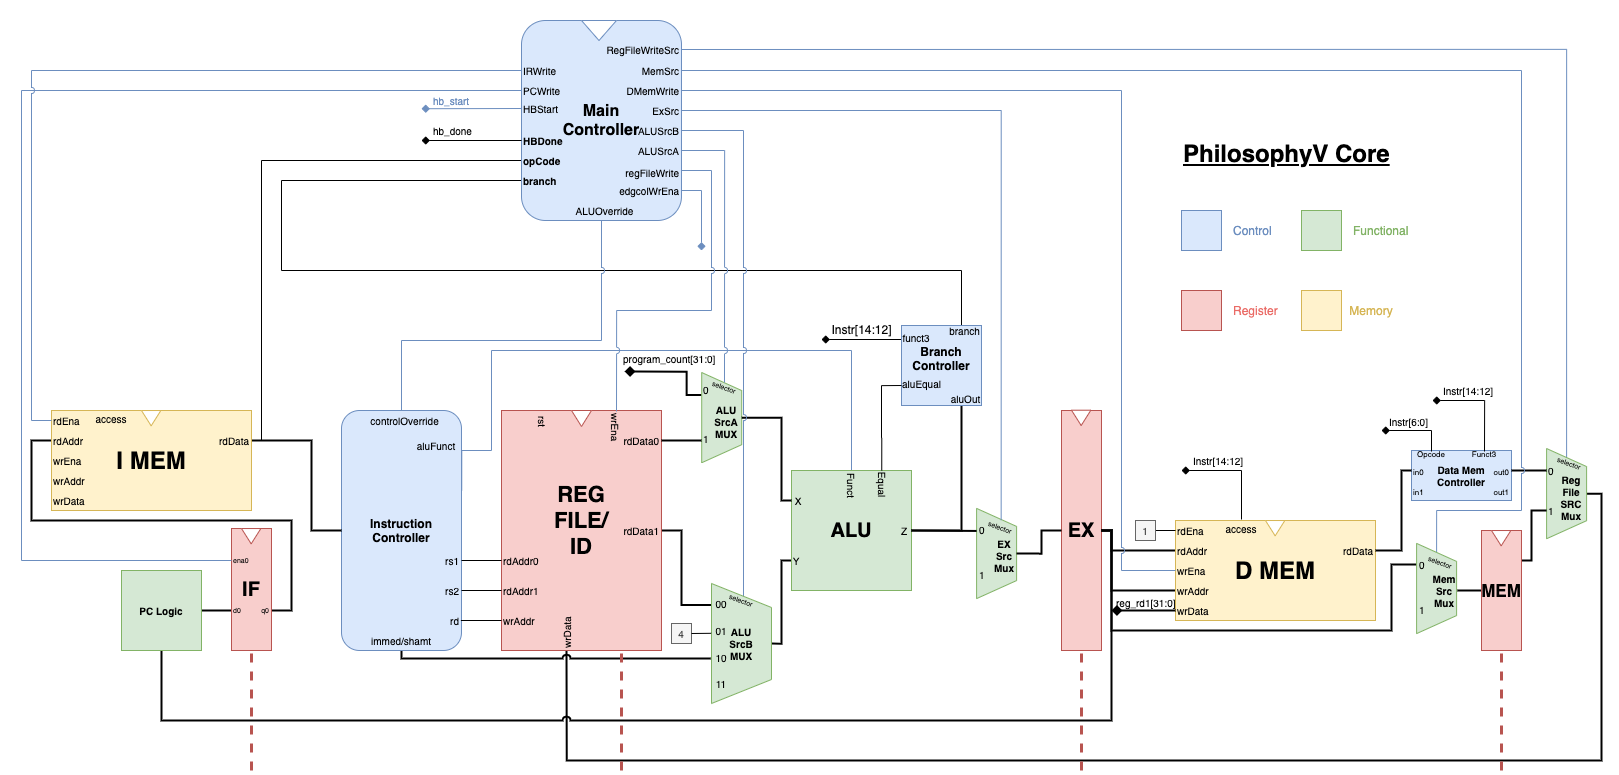
\includegraphics[width=0.7\linewidth]{chapters/chapter4/img/philv-core.png}
\mycaption{RV32I PhilosophyV Schematic}{}
\label{fig:philv-core}
\end{centering}
\end{figure}
 
\thispagestyle{empty}
\newpage



\newpage
% @Author: AnthonyKenny98
% @Date:   2020-03-01 15:57:31
% @Last Modified by:   AnthonyKenny98
% @Last Modified time: 2020-04-10 06:41:50
\begin{figure}[H]
\begin{centering}
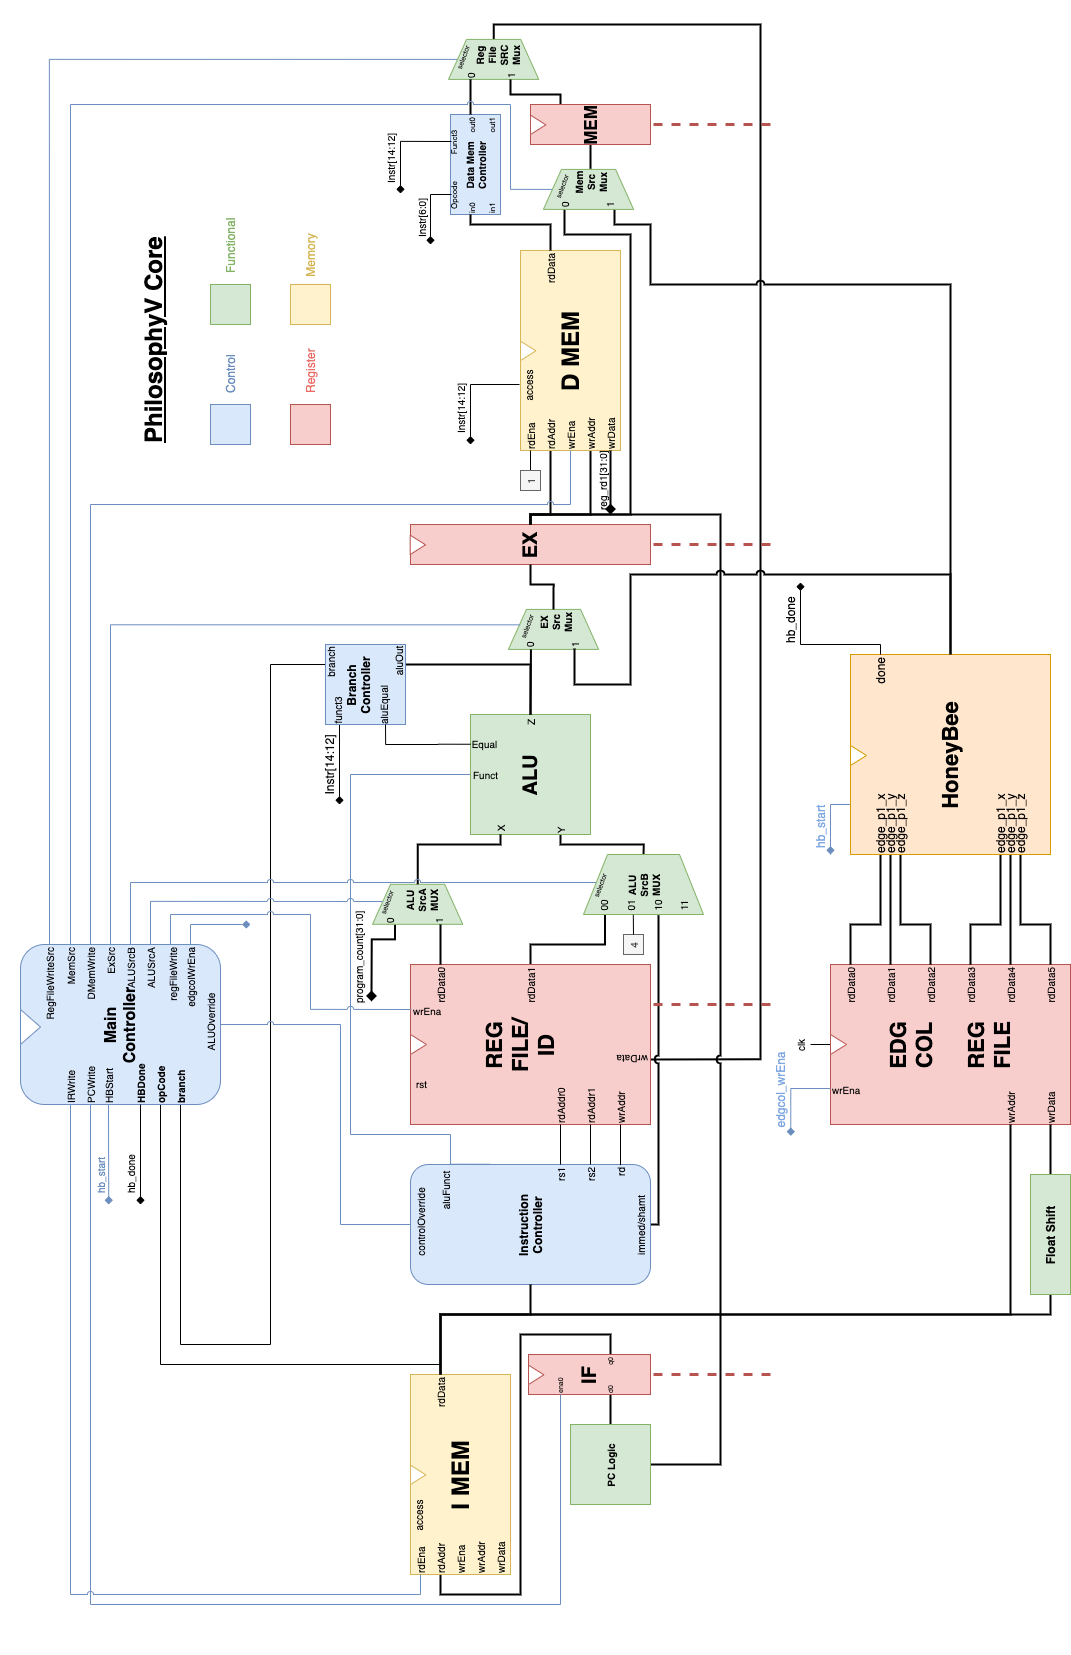
\includegraphics[width=0.9\linewidth]{chapters/chapter4/img/philv-core-rv32i_Xedgcol.png}
\mycaption{RV32I\_Xedgcol PhilosophyV Schematic}{}
\label{fig:philv-core}
\end{centering}
\end{figure}
 
\thispagestyle{empty}
\newpage

\end{appendices} 

\bibliography{\bibliographyName}
\bibliographystyle{ieeetr}

\clearpage 
\newpage

\includepdf{budget}

\end{document}
